%%%%%%%%%%%%%%%%%%%%%
% Type of document: %
%%%%%%%%%%%%%%%%%%%%%
\documentclass[a4paper,11pt]{report}

%%%%%%%%%%%%%%%%%%%%%
% My usual settings %
%%%%%%%%%%%%%%%%%%%%%
\usepackage{JB_config_article}

%%%%%%%%%%%%%%%%%%%%%%%
% Headers and footers %
%%%%%%%%%%%%%%%%%%%%%%%
%%% Color definition:
\definecolor{lgray}{gray}{0.6}

\usepackage{fancyhdr}
\renewcommand{\headrulewidth}{0pt}
\lhead{}
\rhead{}
\lfoot{\vspace{0.3cm}\small\color{lgray}Research report, UCL Department of Statistical Science}
\rfoot{\vspace{-0.3cm}
\includegraphics[width=1.5cm]{ucl.jpg}
\hspace{0.5cm}

\includegraphics[width=1.5cm]{dstl.png}}
\pagestyle{fancy}

%%%%%%%%%%%%%%%%%%%%%%%%%%%
% Location of the figures %
%%%%%%%%%%%%%%%%%%%%%%%%%%%
\graphicspath{{Images/}} 

%%%%%%%%%%%%%%%%%%%%%%%%%%%%%%%%%%%%%%%%%%%%%%%%%%%%%%%%%%%%%%%%%%%%%%%%%%%%%%%%%%%%%%%%%%%%%%%%%%%%%%%%%%%%%%%%%%%%%%%%%%%%%%%%%%%%%%%%%%%%%%%%%%%%%%%%%%%%%%%%%%%%%%%%%%%%%%%%%%%%%%%%%%%%%%%%%%%%%%%%%%%%%%%%%%%%%%%%%%%%%
%%%%%%%%%%%%%%%%%%%%%%%%%%%%%%%%%%%%%%%%%%%%%%%%%%%%%%%%%%%%%%%%%%%%%%%%%%%%%%%%%%%%%%%%%%%%%%%%%%%%%%%%%%%%%%%%%%%%%%%%%%%%%%%%%%%%%%%%%%%%%%%%%%%%%%%%%%%%%%%%%%%%%%%%%%%%%%%%%%%%%%%%%%%%%%%%%%%%%%%%%%%%%%%%%%%%%%%%%%%%%
%%%%%%%%%%%%%%%%%%%%%%%%%%%%%%%%%%%%%%%%%%%%%%%%%%%%%%%%%%%%%%%%%%%%%%%%%%%%%%%%%%%%%%%%%%%%%%%%%%%%%%%%%%%%%%%%%%%%%%%%%%%%%%%%%%%%%%%%%%%%%%%%%%%%%%%%%%%%%%%%%%%%%%%%%%%%%%%%%%%%%%%%%%%%%%%%%%%%%%%%%%%%%%%%%%%%%%%%%%%%%
%%%%%%%%%%%%%%%%%%%%%%%%%%%%%%%%%%%%%%%%%%%%%%%%%%%%%%%%%%%%%%%%%%%%%%%%%%%%%%%%%%%%%%%%%%%%%%%%%%%%%%%%%%%%%%%%%%%%%%%%%%%%%%%%%%%%%%%%%%%%%%%%%%%%%%%%%%%%%%%%%%%%%%%%%%%%%%%%%%%%%%%%%%%%%%%%%%%%%%%%%%%%%%%%%%%%%%%%%%%%%
%%%%%%%%%%%%%%%%%%%%%%%%%%%%%%%%%%%%%%%%%%%%%%%%%%%%%%%%%%%%%%%%%%%%%%%%%%%%%%%%%%%%%%%%%%%%%%%%%%%%%%%%%%%%%%%%%%%%%%%%%%%%%%%%%%%%%%%%%%%%%%%%%%%%%%%%%%%%%%%%%%%%%%%%%%%%%%%%%%%%%%%%%%%%%%%%%%%%%%%%%%%%%%%%%%%%%%%%%%%%%
% Start the document
\begin{document}

	%% Cover page:
	\begin{titlepage}
	%\vspace*{1cm}
		\hspace{-1.5cm}
\includegraphics[width=9cm,height= 3cm]{ucl.jpg}
		\hfill{
		  \raggedleft 
\includegraphics[width=5cm]{dstl.png}
		}
		\vspace*{5cm}
	
		\begin{center}
			\begin{sc} 	
				%%% Title:
				\huge SCATTERING CONVOLUTIONAL HIDDEN MARKOV TREES
				\vspace*{0.2cm}
				%%% Subtitle:
				\\ \large IMAGE REPRESENTATION AND SCATTERING TRANSFORM MODELLING
				\vspace*{2cm}
			\end{sc}
			%%% Author:
			\\ \LARGE Jean-Baptiste REGLI
			\vspace*{0.2cm}
			%%% Date
			\\ \large 2014-2015
		\end{center}
		%\vspace*{5cm}

		%%% Supervisors:
		\vfill
		\begin{center}
			\vspace*{1cm}
			\Large RESEARCH REPORT
			\vspace*{0.5cm}
			\\ \large Academic supervisor: James Nelson 
			\\ \large Sponsor: Dstl/UCL Impact studentship
			
			\vspace*{1cm}
			\Large UCL
			\\ \normalsize Department of Statistical Science
			\\ London
		\end{center}
	\end{titlepage}
	\clearpage

	\vfill	
		
	% Blank page
	\newpage
	\thispagestyle{empty}
	\mbox{}
 
	% Table of contents
	\renewcommand{\contentsname}{Contents:}
	\setcounter{tocdepth}{2}% Allow only \chapter \section \subsection and \subsubsection in ToC
	\tableofcontents
	
	\clearpage

	% List of figures
	\renewcommand{\listfigurename}{List of figures:}
	\listoffigures

%%%%%%%%%%%%%%%%%%%%%%%%%%%%%%%%%%%%%%%%%%%%%%%%%%%%%%%%%%%%%%%%%%%%%%%%%%%%%%%%%%%%%%%%%%%%%%%%%%%%%%%%%%%%%%%%%%%%%%%%%%%%%%%%%%%%%%%%%%%%%%%%%%%%%%%%%%%%%%%%%%%%%%%%%%%%%%%%%%%%%%%%%%%%%%%%%%%%%%%%%%%%%%%%%%%%%%%%%%%%%
%%%%%%%%%%%%%%%%%%%%%%%%%%%%%%%%%%%%%%%%%%%%%%%%%%%%%%%%%%%%%%%%%%%%%%%%%%%%%%%%%%%%%%%%%%%%%%%%%%%%%%%%%%%%%%%%%%%%%%%%%%%%%%%%%%%%%%%%%%%%%%%%%%%%%%%%%%%%%%%%%%%%%%%%%%%%%%%%%%%%%%%%%%%%%%%%%%%%%%%%%%%%%%%%%%%%%%%%%%%%%
%%%%%%%%%%%%%%%%%%%%%%%%%%%%%%%%%%%%%%%%%%%%%%%%%%%%%%%%%%%%%%%%%%%%%%%%%%%%%%%%%%%%%%%%%%%%%%%%%%%%%%%%%%%%%%%%%%%%%%%%%%%%%%%%%%%%%%%%%%%%%%%%%%%%%%%%%%%%%%%%%%%%%%%%%%%%%%%%%%%%%%%%%%%%%%%%%%%%%%%%%%%%%%%%%%%%%%%%%%%%%
\chapter{Introduction:}
	\label{chap:Intro}
	
	Nowadays statistical signal processing and machine learning methods are applied to a wide range of problems from prediction to optimal control. While some of those applications involves low-dimensional data, full branches of those fields are dedicated to studying high-dimensional inputs. Such problems are focused on studying data living in a complex input space and can be found in field such as image or speach processing, DNA decoding or text document mining. This field has known a regain in popularity lately firstly because, over the couple last decades data got cheaper to collect. This is mainly due to the progresses made on digital cameras, microphones and other sensors for signal acquisition. Second the cost of data storage massively decrease during that time. And finally the computational power available today allows to use more computationally intensive methods on larger datasets. Hence methods to leverage those data have been developed across the range of applications in machine learning and statistical signal processing.\\
	
	The standard approach when working with high dimensional signals can be expressed as a two step procedure. First the data are projected in a feature space where the task at hand (classification, regression...) is simplified. Then prediction is done using a simple predictor in this new representational space. Predictors such as logistic regression or linear Support vector Machine are common choices. The mapping can either be hand-build ---\eg Fourier transform, wavelet transform--- or learned. In the last decade methods for learning the projection have drastically improved under the impulsion of the so called deep learning methods. Deep neural networks (sometime enriched by convolutional architecture) have been able to learn very effective representations for a given dataset and a given task. Such method have achieved state of the art on many standard problems as well as real world applications. And this despite using a very simple prediction mechanism ---on top of a very clever projection method.\\
	
	This document proposes a method combining a recently proposed deterministic analytically tractable transformation inspired by deep convolutional to a probabilistic graphical model in order to create a powerful probabilistic tool to handle high dimensional prediction problems. In a similar fashion to the work done by Crouse on wavelet trees~\citep{crouse1998wavelet}, we propose to describe Mallat's scattering convolutional scattering transform~\citep{bruna2010classification} using a hidden Markov tree. Doing so we develop a new framework to model high-dimensional inputs. As opposed to the commonly used simple classification method, once trained our model can tackle prediction problems but also other inference tasks ---\eg generation, sensitivity analysis...
	
	\section{Signal representation:}
		\label{sec:Intro/Need}
				
		Consider the problem of learning the labelling function, say, $f$ given $N$ sampled training values $\{\bfx_{i}, y_{i}=f(\bfx_{i})\}_{i\leq N}$ where  for all $i \in \llbracket 1 , N \rrbracket$, $\bfx_{i} =\{ x[1] \, \dots \, x[d] \}$ with $d \sim 10^{6}$, $x[.] \in \dsR$ and $y_{i} \in \dsN$. Such signals are, for example, speech waveforms, digital photographies but also electrocardiograms, sonar imagery and many others.\\

		\begin{figure}[h]
			\centering
			\begin{subfigure}[t]{0.48\textwidth}
				\centering
				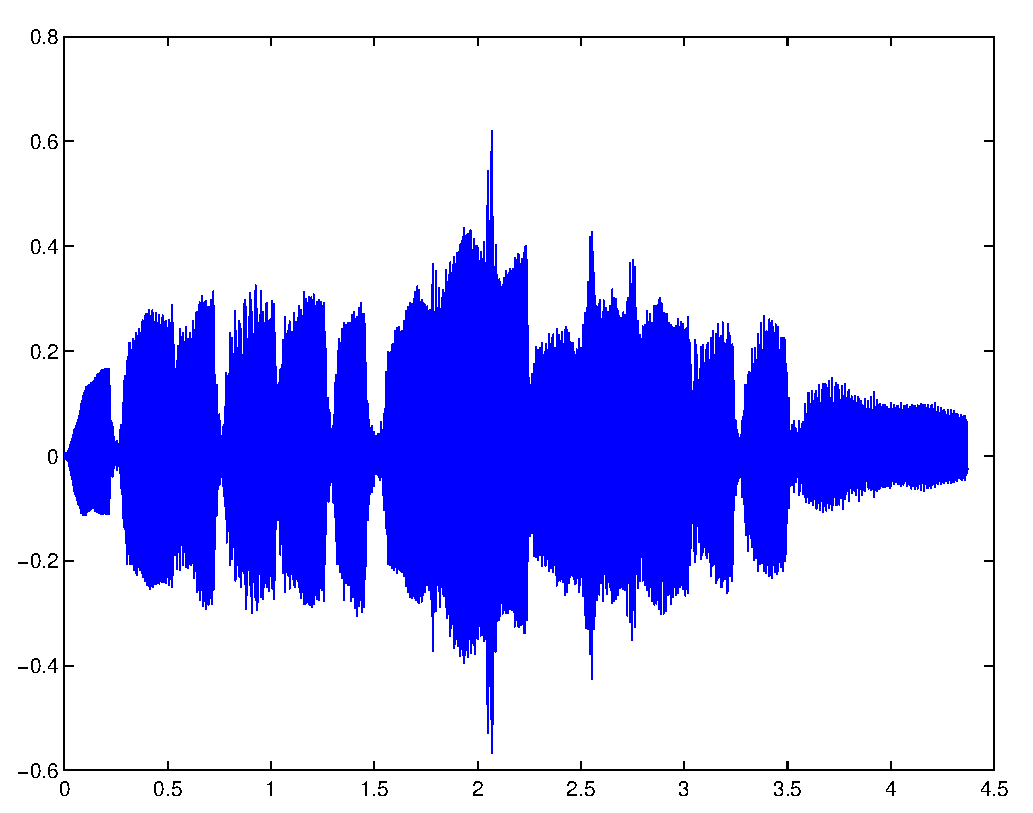
\includegraphics[height=2.2in]{waveform_flute.eps}
				\caption{Sound of a flute}
			\end{subfigure}%
			~ 
			\begin{subfigure}[t]{0.48\textwidth}
        \centering
        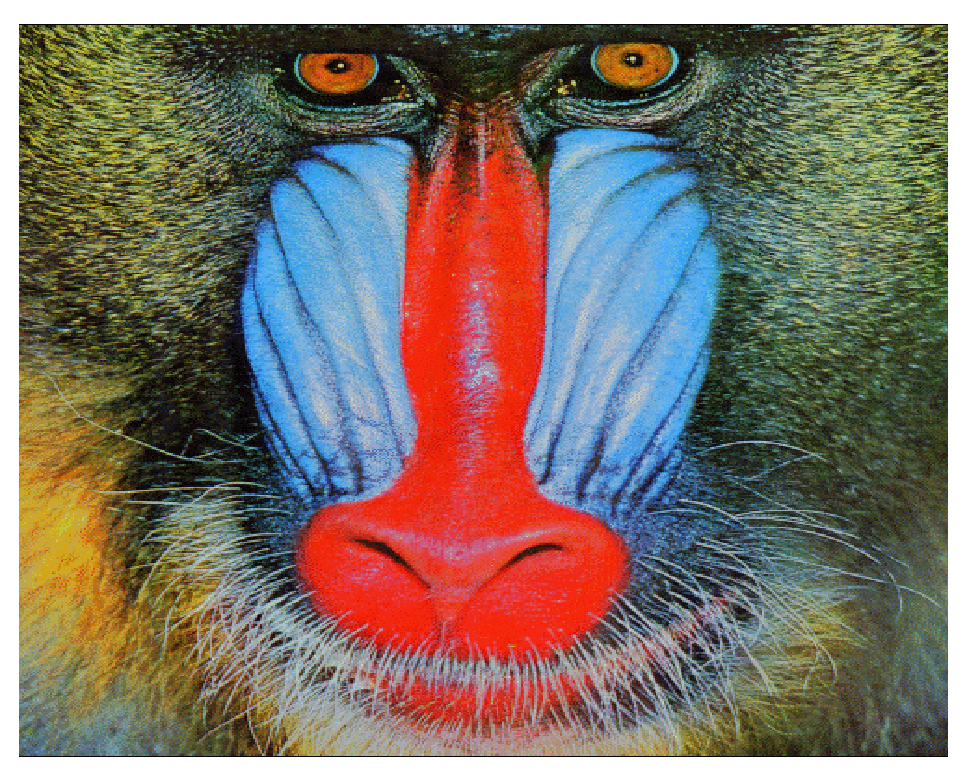
\includegraphics[height=2.2in]{im_mandrill.eps}
        \caption{Picture of a mandrill}
			\end{subfigure}
			\caption{High dimensional signals.}
			\label{fig:highDim signals}
		\end{figure}
		
		A naive solution to this problem would be to infer the class of a new realization $\bfx^{new}$ by looking at its neighbours in a similar fashion to K-Nearest Neighbours (KNN), for example. This approach is sound for low-dimensional problems~\citep{cover1967nearest}. However it shows limitations in high dimensional cases~\citep{beyer1999nearest} as the number of samples required to find a neighbour of a new realization $\bfx^{new}$ grows exponentially with the number of dimensions. This issue is known in the statistical learning community as the curse of dimensionality.\\
			
		One can make the assumption that the signal $\bfx$ belongs to a manifold $\Omega$ of $\dsR^{d}$ and this leads to two types of problems. The subset $\Omega$ can be low dimensional and the curse of dimensionality is avoided once the manifold has been isolated. The task at hand is thus a manifold learning problem~\citep{lin2008riemannian} \citep{zhang2012adaptive} or a sparse dictionary representation problem~\citep{kreutz2003dictionary}. However for complex signals, the manifold $\Omega$ is also expected to be high dimensional. In this case, in order to simplify the prediction task, one has to reduce the volume of the signal space without loosing crucial information required to characterize those signals. Hence one has to reduce the volume of $\Omega$ according to the properties of the classification function $f$.\\
		
		A mapping $\Phi$ is sought which represents the signal in a new space such that the classification task is simpler. The space should not only capture the main information and discriminatory content in the data but it should also remain stable with respect to appropriate transformations and deformations. Before providing a formal mathematical description of this mapping, it is instructive to consider the following intuitive example.
    
		\subsection{Intuition:}
      \label{sec:Intro/Signal rep/Intuition}
      
      Properties of a ``good'' representation for classification can be intuited by looking how humans handle the classification/labelling of visual stimulus and what the elements ensuring good generalization capacities are. Following this approach, one can intuit the following properties:\\
            
			\begin{itemize}
				\item The projection has to be informative enough to permit classification. This means ensuring that $\Phi$ preserves separability between the different classes.\\

				\item The mapping also has to be invariant to translations. Indeed to a human observer, there is no difference in the information carried by a signal if it has been shifted. This means that the transformation $\Phi$ has to provide close, if not equal, outputs for shifted versions of the same signal.\\
		
				\begin{figure}[h]
					\centering
					\begin{subfigure}[t]{0.48\textwidth}
						\centering
						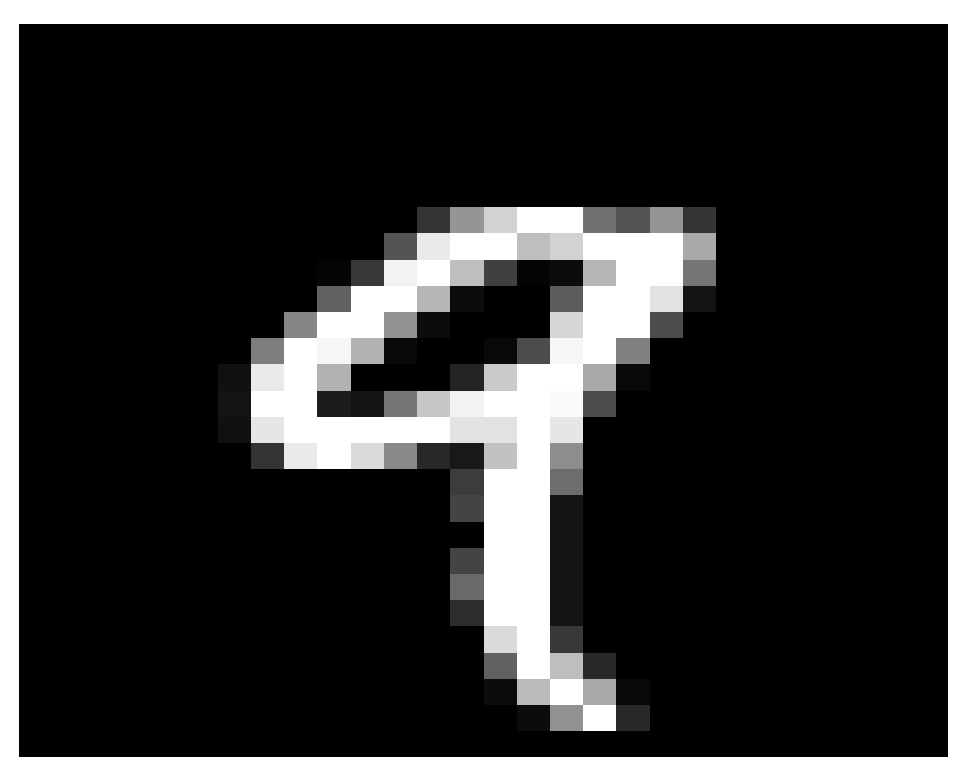
\includegraphics[height=2.3in]{im_nine_ori.eps}
					\end{subfigure}%
					~ 
					\begin{subfigure}[t]{0.48\textwidth}
						\centering
						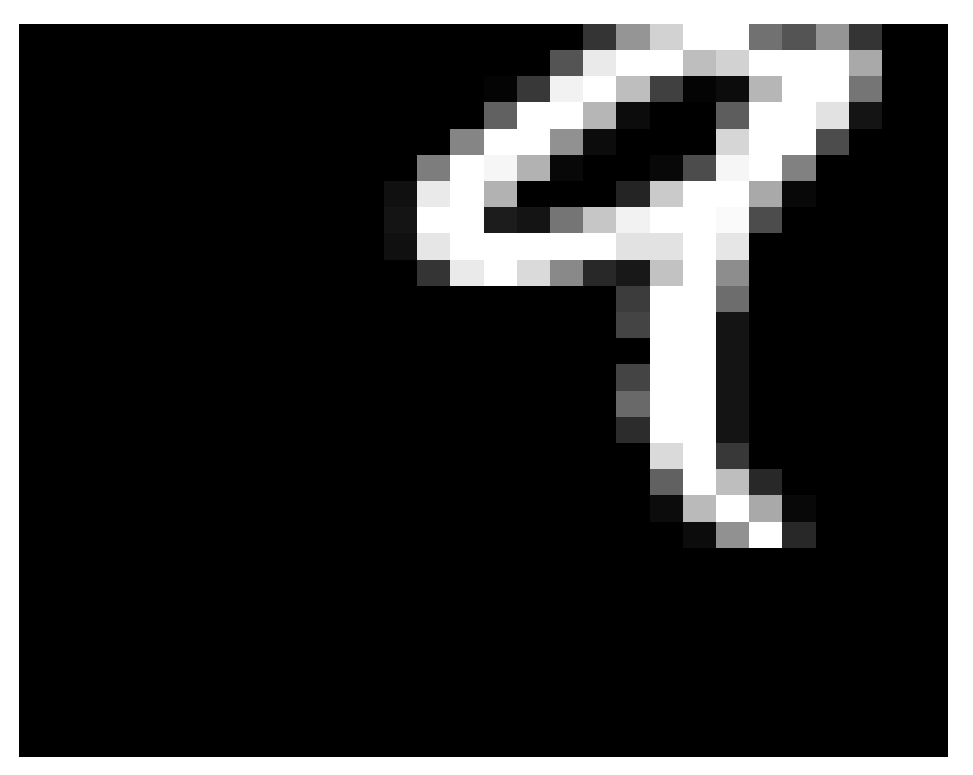
\includegraphics[height=2.3in]{im_nine_trl.eps}
					\end{subfigure}
					\caption[Translation invariance.]{\centering Translation invariance: Huamns can easily tell that those two images are from the same class.}
					\label{fig:Illustration translation invariance}
				\end{figure}
	
				\item To some extend the mapping has to be stable under deformations. Again, humans are still able to recognize a signal if it has undergone ---small--- deformations. Yet if the morphings are too important the information content of the signal can be lost (see Figure~\ref{fig:Illustration stability deformations}). This means that to a certain degree the projections of morphed realizations of the same signal should be mapped to a same region of the representational space. However one needs to define a limit to this invariance to ensure that the representation created is still informative enough.\\
				
				\begin{figure}[h]
					\centering
					\begin{subfigure}[t]{0.48\textwidth}
						\centering
						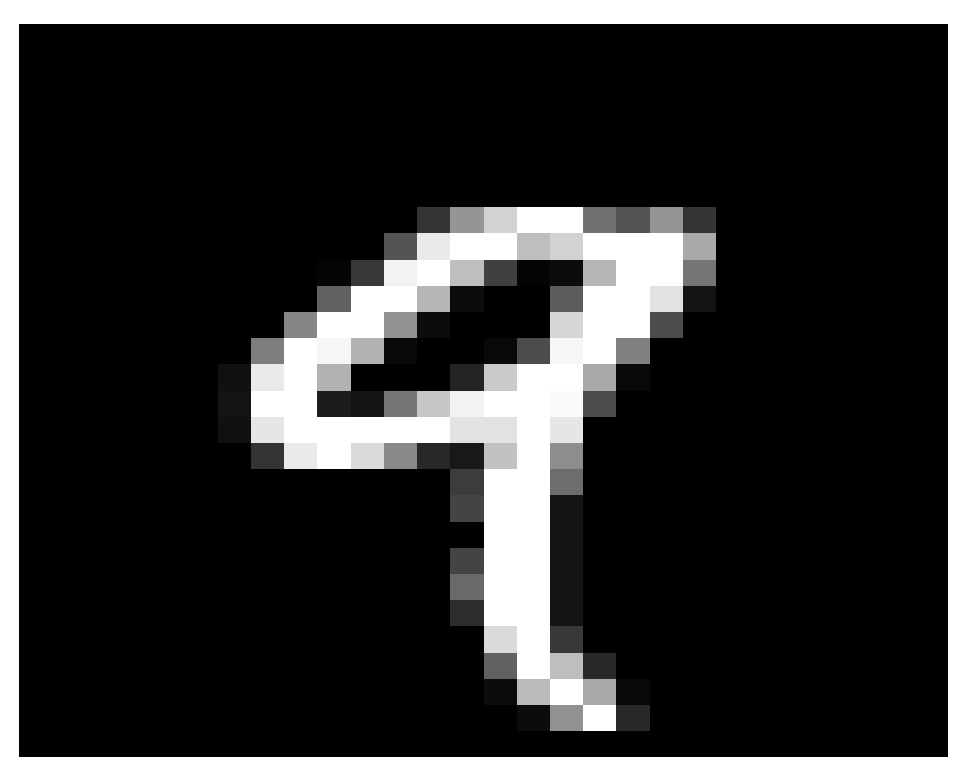
\includegraphics[height=2.3in]{im_nine_ori.eps}
						\caption{\centering Original}
					\end{subfigure}%
					~
					\begin{subfigure}[t]{0.48\textwidth}
						\centering
						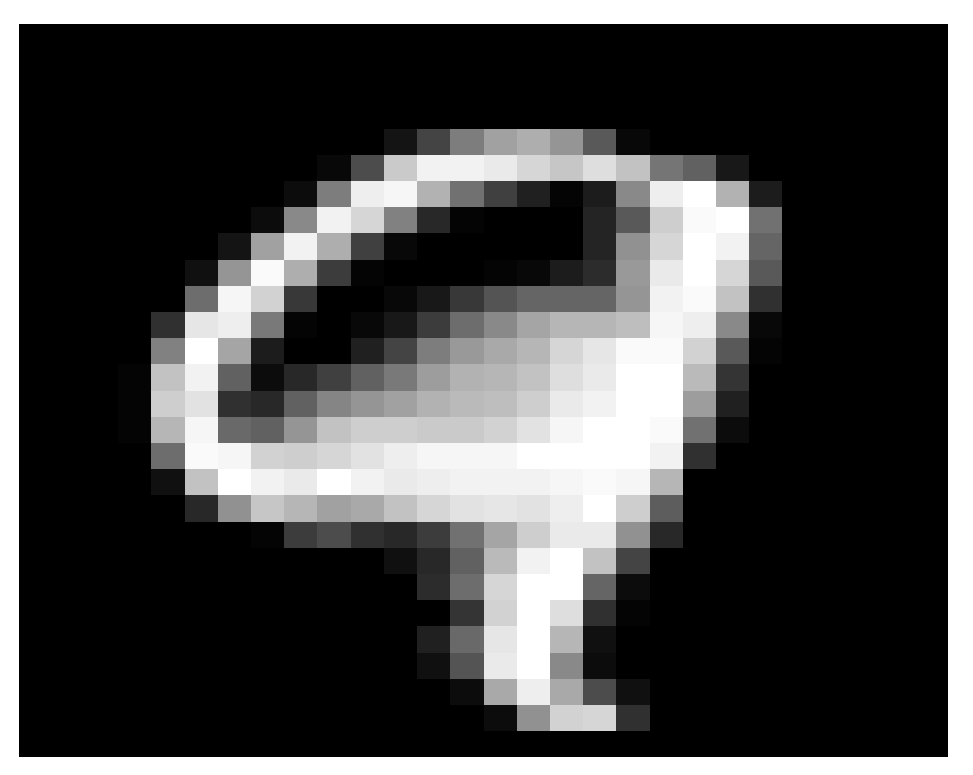
\includegraphics[height=2.3in]{im_nine_def_Vsmall.eps}
						\caption{\centering Light deformation}
					\end{subfigure}%
					\\
					~
					\begin{subfigure}[t]{0.48\textwidth}
						\centering
						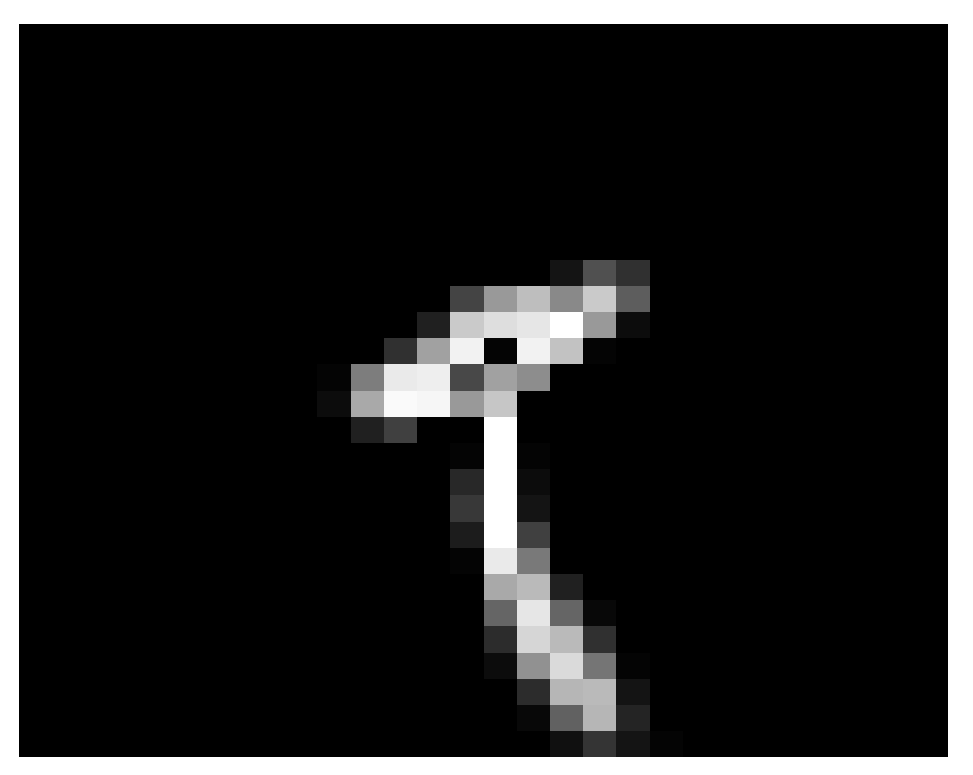
\includegraphics[height=2.3in]{im_nine_def_small.eps}
						\caption{\centering Important deformation}
					\end{subfigure}
					~ 
					\begin{subfigure}[t]{0.48\textwidth}
						\centering
						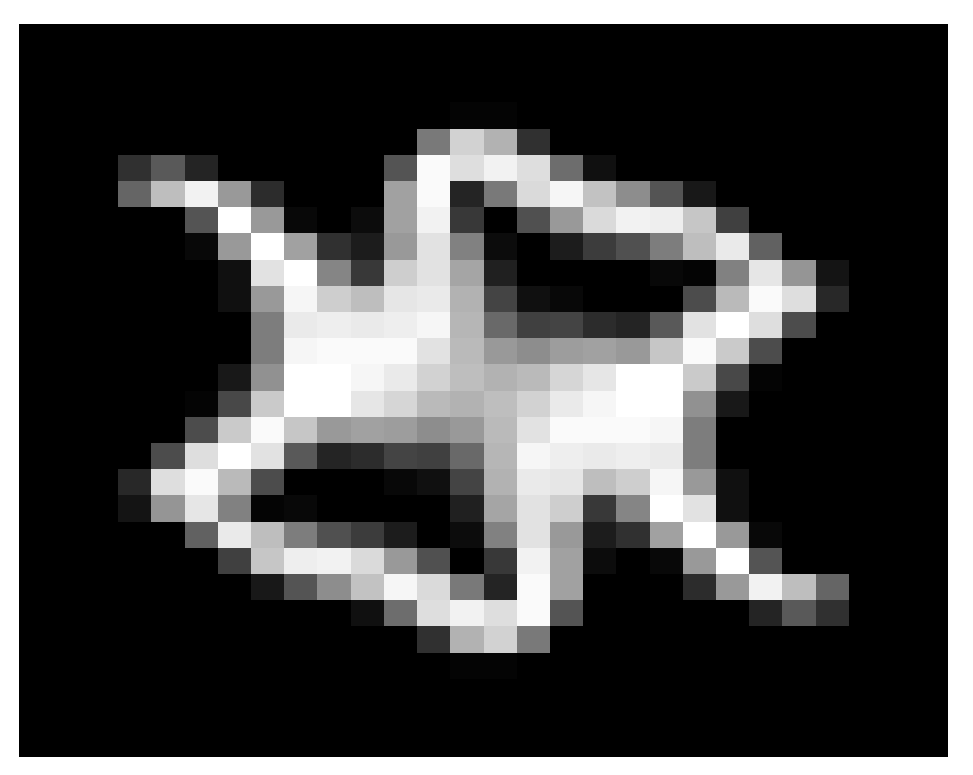
\includegraphics[height=2.3in]{im_nine_def_big.eps}
						\caption{\centering Loss of information}
					\end{subfigure}
					
					\caption[Stability to deformations.]{\centering Stability to deformations: Huamns can easily tell that (a) and (b) are from the same class. (c) can still be recognized even though it is slightly more challenging. For (d) the informative content is lost.}
					\label{fig:Illustration stability deformations}
				\end{figure}
				
				\item Again to a certain degree the projection has to be invariant to rotations. Only local invariant to rotation is wanted because excessive rotation applied to the original signal can be destructive for the information carried (see Figure~\ref{fig:Illustration rotation invariance}). Solutions based on the method described in this document exist~\citep{sifre2013rotation}~\citep{oyallon2014deep} but they are still work in progress and thus they will not be addressed nor used in this review. 

				\begin{figure}[h]
					\centering
					\begin{subfigure}[t]{0.48\textwidth}
						\centering
						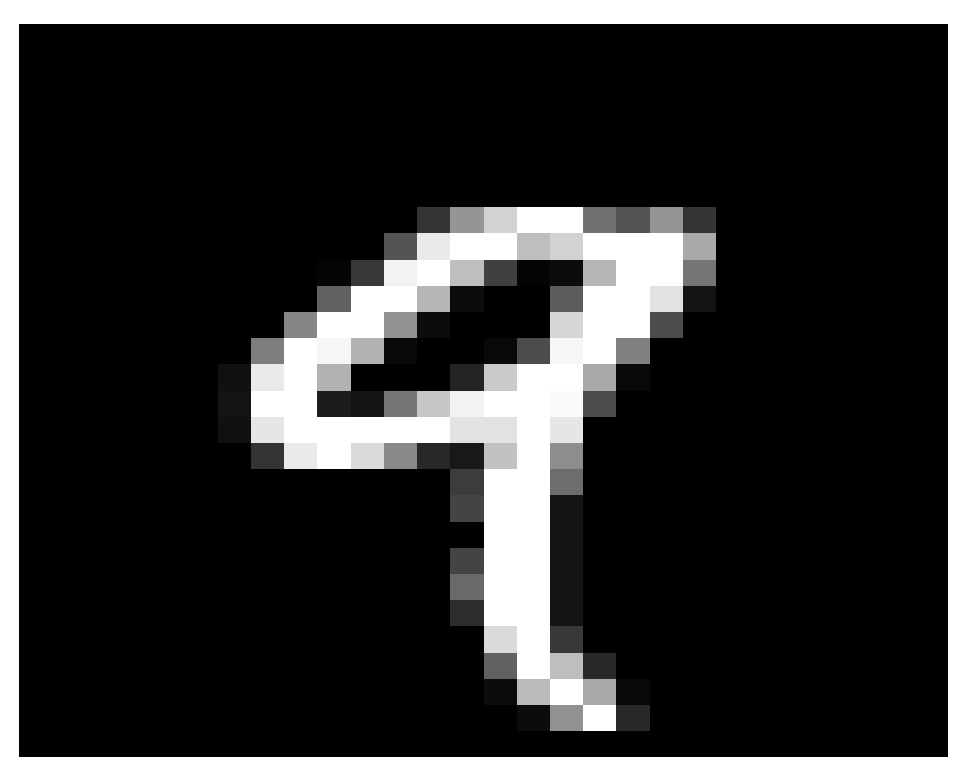
\includegraphics[height=2.3in]{im_nine_ori.eps}
						\caption{\centering Original}
					\end{subfigure}%
					~
					\begin{subfigure}[t]{0.48\textwidth}
						\centering
						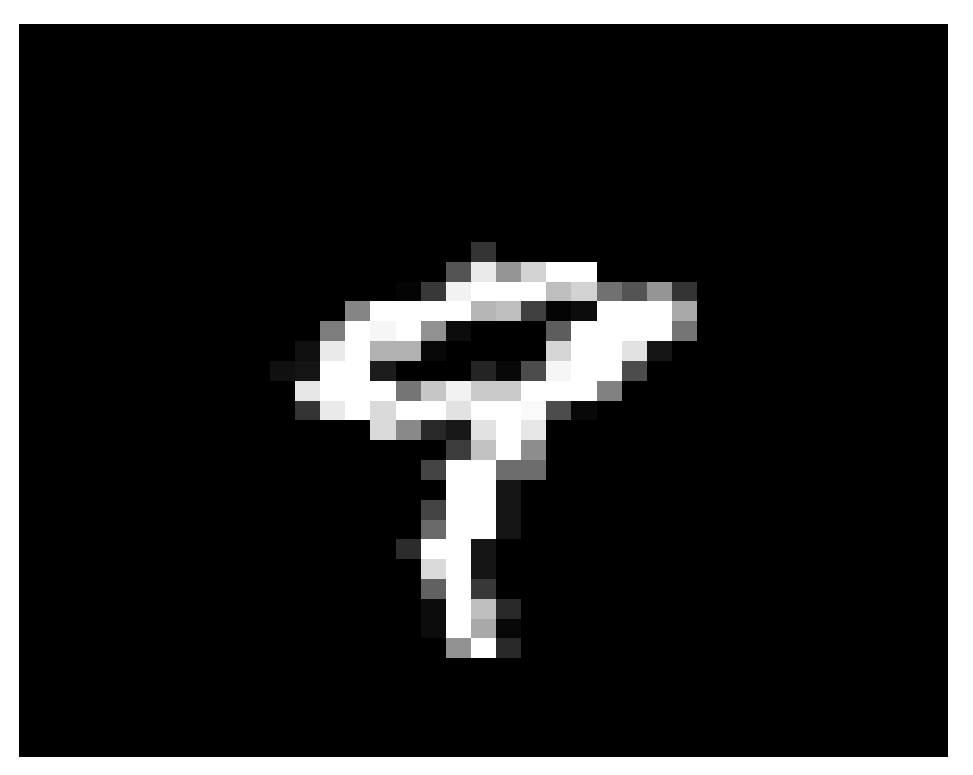
\includegraphics[height=2.3in]{im_nine_rot15.eps}
						\caption{\centering Small rotation}
					\end{subfigure}%
					\\ 
					~
					\begin{subfigure}[t]{0.48\textwidth}
						\centering
						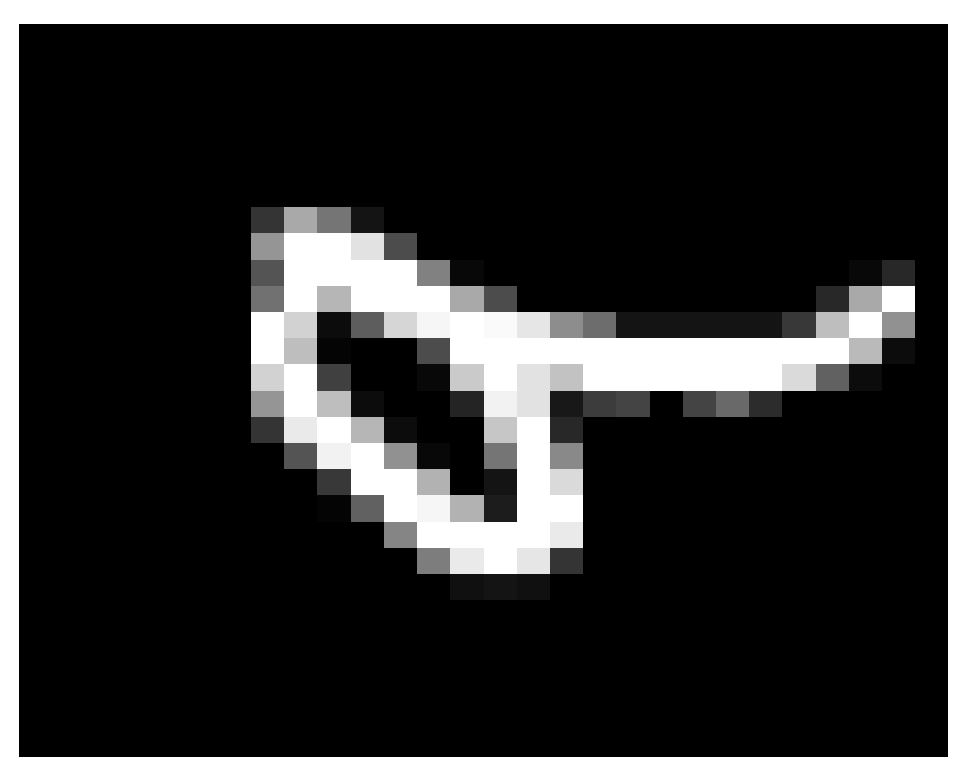
\includegraphics[height=2.3in]{im_nine_rot90.eps}
						\caption{\centering Important rotation}
					\end{subfigure}
					
					\caption[Rotation invariance.]{\centering Rotation invariance: Huamns can easily tell that (a) and (b) are from the same class. (c) could be either a  `6' or a `9'.}
					\label{fig:Illustration rotation invariance}
				\end{figure}
			
			\end{itemize}
			
      
		\subsection{Formalization:}
      \label{sec:Intro/Signal rep/Formalization}
      
			Throughout, attention is restricted to signal represented by square-integrable $d$-dimensional functions over the real, namely $\bfx \in \mcalL^{2}(\dsR^{d})$. For more accuracy, the classification function is split in two stages. $f$ now denotes the soft classification function, \ie $f(\bfx) \in \dsR^{K}$ where $K$ is the dimension of the mapping space, and represents the distance to the separating surface. $h$ is the labelling function such that $y=h \circ f(\bfx)$ is now the label associated to a signal $\bfx$. To be informative enough, a representation must preserve separability between elements of different classes. This is encapsulated by the following definition.
      
			\begin{defn} \textbf{(Separability preservation)}\\
				A representation $\Phi$ preserves separability if all elements of two different classes are distant of at least a margin $C$ in the representation space,
				\begin{equation*}
					\forall x,x' \in \dsR^{d} \;\;\; \exists C \in \dsR^{K} \;\;\; \st \;\;\; h \circ f(x) \neq h \circ f(x') \;\; \Rightarrow \;\; \norm{\Phi(x)-\Phi(x')} \geq C^{-1}
				\end{equation*}
				where $K$  is the dimension of the mapping space.
				\label{def:Separability}
			\end{defn}
			
      Translations in the input space should not affect the representation. In this document let $L_{(.)}$ denote the translation operator for the function in $\mcalL^{2}(\dsR^{d})$, \ie for $\bfx \in \mcalL^{2}(\dsR^{d}) \;\; \text{and} \;\; u,c \in \dsR^{d} \times \dsR^{d} \;\;\;\; L_{c}\bfx(u) = \bfx(u-c)$. A mapping $\Phi$ is translation invariant ---respectively canonical translation invariant ---if it maps a translated signal to the same point as its original version.

      \begin{defn} \textbf{(Translation invariance)}\\ 
				An operator $\Phi: \mcalL^{2}(\dsR^{d}) \rightarrow \mcalH$, where $\mcalH$ is a Hilbert space, is translation invariant if:
	      	\begin{equation*}
			  		\forall c \in \dsR^{d} 
			  		\;\;\; \text{and}  \;\;\;
			  		\forall \bfx \in \mcalL^{2}(\dsR^{d}) \;\;\;
			  		\Phi(L_{c}\bfx) = \Phi(\bfx).
				\end{equation*}
				\label{def:Translation invariance - intuition}
      \end{defn}
      \vspace{-30pt}

      \begin{defn} \textbf{(Canonical translation invariant)}\\ 
				An operator $\Phi: \mcalL^{2}(\dsR^{d}) \rightarrow \mcalH$, where $\mcalH$ is a Hilbert space, is canonical translation invariant if:
        \begin{equation*}
			  		\forall \bfx \in \mcalL^{2}(\dsR^{d}) \;\;\;
			  		\Phi(L_{a}\bfx) = \Phi(\bfx) 
			  		\;\;\; \text{where} \; a \in \dsR^{d} \; \text{is function of} \; \bfx.
				\end{equation*}
				\label{def:Canonical translation invariance - intuition}
      \end{defn}
      
      For the standard representation operators, instabilities to deformations are known to appear ---especially at high frequencies. To prevent this, one would like the representation to be non-expansive.
      
      \begin{defn} \textbf{(Non-expensive representation)}\\
				A representation $\Phi$ is non-expensive if,
				\begin{equation}
			  		\forall \bfx,\bfx' \in \mcalL^{2}(\dsR^{d}) \;\;\; 
			  		\norm{\Phi(\bfx) - \Phi(\bfx')} \leq \norm{\bfx-\bfx'}.
				\end{equation}
				\label{def:Non-expansivity - intuition}
      \end{defn}
      
      The local stability to deformations of a non-expansive operator can be expressed as its Lipschitz continuity to the action of deformations close to translations~\citep{mallat2012gis}. Such a diffeormorphism can be expressed as,
      \begin{equation*}
      		\begin{split}
      			L_{\tau}	: \; & \mcalL^{2}(\dsR^{d}) \rightarrow \mcalL^{2}(\dsR^{d})\\
      							  & \;\;\;\; \bfx \;\;\;\;\; \rightarrow  \bfx((.) - \tau(.))
				\end{split}
      \end{equation*}

			where $\tau(u) \in \dsR^{d}$ is a displacement field.
			
			\begin{defn} \textbf{(Lipschitz continuous)}\\
				A non expansive operator $\Phi$ is said to be Lipschitz continuous to the action of $\mcalC^{2}$ diffeomorphisms if for any compact $\Omega \subset \dsR^{d}$ there exists $C$ such that for all $f \in \mcalL^{2}(\dsR^{d})$ supported in $\Omega$ and all $\tau \in \mcalC^{2}(\dsR^{d})$,
				\begin{equation}
					\norm{\Phi(\bfx) - \Phi(L_{\tau}\bfx)}_{\mathit{H}} \leq 
					C \norm{\bfx} \left(\sup_{u \in \dsR^{d}} \abs{\nabla \tau(u)} + \sup_{u \in \dsR^{d}} \abs{\mathit{H}\tau(u)}\right)
					\label{eq:Lipschitz continuity}
				\end{equation}
				\label{pty:Lipschitz continuity - intuition}
							
				where $\nabla \tau(u)$ is a matrix whose norm $\abs{\nabla \tau(u)}$ measures the deformation amplitude at point $u$, $\mathit{H}\tau(u)$ is the Hessian matrix of the deformation and its sup-norm $\abs{\mathit{H}\tau(u)}$ measures the smoothness of the deformation.\\
      \end{defn}

      Hence such a Lipschitz continuous operator $\Phi$ is almost invariant to deformations by $\tau(.)$, up to the first and second order deformation terms. Equation~\ref{eq:Lipschitz continuity} also implies that $\Phi$ is invariant to global translations but this is already enforced by the translation invariance requirement.\\ 
      
%       This document and more precisely Section~\ref{chap:ST} introduces an analytically tractable, deterministic wavelet based transformation fulfilling all the properties mentioned in this section.

    \subsection{State of the art:}
      \label{sec:Intro/Signal rep/State of the art}      
          
			A common representational method is the modulus of the Fourier transform. To a certain extend this operator is informative enough to allow discrimination between different types of signals~\citep{baker2014using}. It is also translation invariant~\citep{bracewell1965fourier}. However it is well known that those operators present instabilities to deformation at high frequencies~\citep{hormander1971fourier} and thus are not Lipschitz continuous to the action of diffeomorphisms.\\
      
			Wavelet transform is another popular representation method. Again it provides a representation suitable for classification of different signals~\citep{de2000using}. Plus by grouping high frequencies into dyadic packet, wavelet operators are stable to ---small--- deformations~\citep{bruna2013invariant}.  %TODO: what does it mean? To be confirm
			
			\begin{equation}
				\begin{matrix}
					W\bfx =
					\begin{pmatrix}
						\bfx \ast \phi \\[0.5em]
						\bfx \ast \psi_{\lambda} \\[0.5em]
					\end{pmatrix}
					\begin{aligned}
						\begin{matrix}
							\rightarrow \text{averaging part}				\\[0.5em]
							\rightarrow \text{high frequency part}	\\[0.5em]
						\end{matrix}
					\end{aligned}
				\end{matrix}
			\end{equation}
		
			However only the averaging part of a wavelet is invariant to translation ans thus wavelets themselves are known to be non-invariant to translations.\\
			
			Another popular signal representation method are the convolutional neural networks~\citep{lecun1995convolutional}. As opposed to the two methods mentioned previously, those operators are not fixed but learned from the data~\citep{simard2003best}. Over the past decade they have provided state of the art results on many standard classification tasks, on image datasets such as \textit{MNIST}, \textit{CIFAR}~\citep{hinton2012improving} and \textit{ImageNet}~\citep{krizhevsky2012imagenet} as well as on speech processing problems such as \textit{TIMIT}~\citep{abdel2012applying}. Those good results are used to advocate that those networks are learning ``good'' representations. However there is no mathematical formalisation of this intuition and it seems that in certain cases they learn representation of the data that are, for example, not invariant to deformations~\citep{szegedy2013intriguing}.\\
			
			\begin{figure}[h]
				\begin{center}
					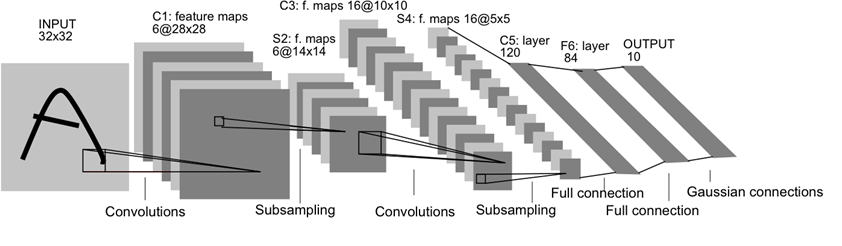
\includegraphics[width=5in]{CNN.png}
					\caption[Convolutional neural network.]{\centering  Convolutional neural network with $3$ convolution/sub-sampling layers and $3$ fully connected layers. }
					\label{fig:SNN}
				\end{center}	
      \end{figure}
			
			         
	\section{Discriminative versus generative models:}
		\label{sec:Intro/Discr vs gen}
		
		Having mapped the data into a representation space, one is left with a ``simpler'' ---yet often still high-dimensional--- prediction problem of an unobserved random variable $y$ --- or random vector $\bfy$--- given a new observation $\bfx^{new}$. In this situation, one can choose between two different types of model.\\
		
		A discriminative model directly expresses the dependencies between the unobserved variable and the observed ones. Which can be seen in a probabilistic framework as model the conditional probability distribution $P(\bfy|\bfx)$. The prediction can then be done directly from the learned function. Examples of such models are Support Vector Machines (SVMs), Neural Networks (NNs) or Conditional Random Fields (CRFs).\\
		
		On the other hand one can use a generative model and specify the joint probability distribution $P(\bfx,\bfy)$. This means that the prediction task ---\ie the conditional probability distribution--- is not straight forward using the model but requires computation via Bayes' rule and specification of a prior $P(\bfx)$. However this also means that those models can be used for more than simply prediction and can for example be use to generate the ``most likely input'' given an output $P(\bfx|\bfy)$. Examples of such models are Naive Bayes classifiers, Restricted Boltzmann Machines (RBMs) or Probabilistic Graphical Models.\\
		
		Because they require extra computation, generative models are usually considered as less efficient for classification than the discriminative ones~\citep{ulusoy2005generative}. However because they model the full joint probability distribution they can be use on a much broader range of tasks. They also have a readily available method for handling missing data, and often better performance when trained on small size training sets~\citep{jordan2002discriminative}.
		
	\section{Outline of the report:}
    \label{sec:Intro/Outline of the report}    
    
    The remainder of this document is organized as follow. Section~\ref{chap:ST} summarizes and explains recent work from St\'ephane Mallat and his group on the Scattering Transform (ST), a wavelet-based operator fulfilling all the properties of what has been defined as a ``good'' representation for signal classification. Section~\ref{chap:PGMs} introduces the concept of Probabilistic Graphical Models (PGMs) as generative models that can be used ---among other tasks--- for classification. Section~\ref{chap:SCHMT} describes how the representation produced by the scattering transform can be modelled by a hidden Markov tree, using what we have named Scattering Convolutional Hidden Markov Trees (SCHMTs). Finally Section~\ref{chap:Exp} provides some examples of application.
        
	\section{Contributions:}
    \label{sec:Intro/Contrib}    
    
    The first two sections of this documents are mostly dedicated at introducing pre-existing notions and concepts that are useful to later construct the scattering convolutional hidden Markov trees. Readers already familiar with Scattering Transforms or Probabilistic Graphical Models can respectively skip Section~\ref{chap:ST} or~\ref{chap:PGMs} and focus on the novelties introduced in Section~\ref{chap:SCHMT} and onward where a framework to model a scattering convolutional network as a hidden Markov tree is presented. This new tool is then tested on classification and segmentation tasks.\\
    
    Note also that even if this document is mainly written using images ---\ie 2-D signals--- as examples, the framework presented is valid for signal of any dimensions with minor adjustments.

    
%%%%%%%%%%%%%%%%%%%%%%%%%%%%%%%%%%%%%%%%%%%%%%%%%%%%%%%%%%%%%%%%%%%%%%%%%%%%%%%%%%%%%%%%%%%%%%%%%%%%%%%%%%%%%%%%%%%%%%%%%%%%%%%%%%%%%%%%%%%%%%%%%%%%%%%%%%%%%%%%%%%%%%%%%%%%%%%%%%%%%%%%%%%%%%%%%%%%%%%%%%%%%%%%%%%%%%%%%%%%%
%%%%%%%%%%%%%%%%%%%%%%%%%%%%%%%%%%%%%%%%%%%%%%%%%%%%%%%%%%%%%%%%%%%%%%%%%%%%%%%%%%%%%%%%%%%%%%%%%%%%%%%%%%%%%%%%%%%%%%%%%%%%%%%%%%%%%%%%%%%%%%%%%%%%%%%%%%%%%%%%%%%%%%%%%%%%%%%%%%%%%%%%%%%%%%%%%%%%%%%%%%%%%%%%%%%%%%%%%%%%%
%%%%%%%%%%%%%%%%%%%%%%%%%%%%%%%%%%%%%%%%%%%%%%%%%%%%%%%%%%%%%%%%%%%%%%%%%%%%%%%%%%%%%%%%%%%%%%%%%%%%%%%%%%%%%%%%%%%%%%%%%%%%%%%%%%%%%%%%%%%%%%%%%%%%%%%%%%%%%%%%%%%%%%%%%%%%%%%%%%%%%%%%%%%%%%%%%%%%%%%%%%%%%%%%%%%%%%%%%%%%%
\chapter{The Scattering transform:}
  \label{chap:ST}
 
	This section describes the construction of a mathematical operator ---the scattering transform (ST)--- designed to generate what has been defined earlier as an interesting representation of signal (see Section~\ref{sec:Intro/Need}). This operator delocalizes signal's informative content into scattering decomposition paths, computed by cascading wavelet/modulus operators through an architecture similar to a Convolutional Neural Network (CNN) where the synaptic weights would be given by a wavelet operator instead of learned.\\ 
	
	The remainder of the chapter is organized as follow. First, Section~\ref{sec:ST/Scattering coefficients} defines the scattering operators. Second, Section~\ref{sec:ST/SCN} describes how those operators can be stacked to create a Scattering Convolutional Network (SCN), an architecture comparable to CNNs. Then Section~\ref{sec:ST/Pties} reviews some of the SCNs' important properties. And finally, Section~\ref{sec:ST/Applications to clf} presents how the scattering transform is usually used in classification tasks.
	      
		\section{Scattering coefficients:}
			\label{sec:ST/Scattering coefficients}

			A two-dimensional directional wavelet is obtained by scaling and rotating a single band-pass filter $\psi$. If one let $G$ be a discrete, finite rotation group of $\dsR^{2}$, multi-scale directional wavelet filters are defined for any scale $j \in \dsZ$ and rotation $r \in G$ by,
      
      \begin{equation}
				\label{eq:multi-scale directional wavelet}
				\psi_{2^{j}r}(u) = 2^{2j} \psi(2^{j}r^{-1}u).
      \end{equation}
      
      To simplify the notations, let now $\lambda = \lambda(j,r) \; \eqdef \; 2^{j}r \; \in \; G \times \dsZ$.\\
      
      A wavelet transform filters the signal $\bfx$ using a family of wavelets $\{\bfx \ast \psi_{\lambda}(u)\}_{\lambda}$ computed from a filter bank of dilated and rotated wavelets having no orthogonality property. This generates a multi-scales and multi-orientations representation of the input signal.\\ 
      
      If $u.u'$ and $\|u\|$ define respectively the inner product and the norm in $\dsR^{2}$, the Morlet wavelet $\psi$ is an example of wavelet given by,
      
      \begin{equation*} 
				\label{eq:Morlet wavelet}
				\psi(u) = C_{1}(e^{iu.\xi} - C_{2}) e^{\|u\|^{2}/(2 \sigma^{2})},
      \end{equation*}

      where $C_{1}$, $\xi$ and $\sigma$ are meta-parameters of the wavelet and $C_{2}$ is adjusted so that $\int \psi(u) du = 0$. Figure~\ref{fig:Morlet wavelet} shows a Morlet wavelet for  $\xi= 3\pi/4$, $\sigma=0.85$ and $C_{1}=1$.\\
      
			\begin{figure}[h]
				\centering
				\begin{subfigure}[t]{0.3\textwidth}
					\centering
					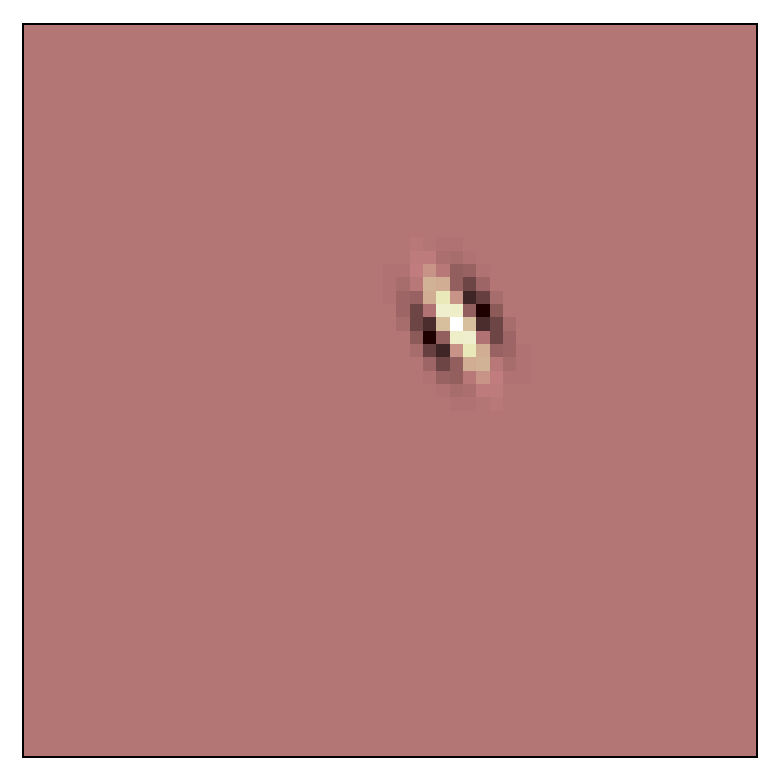
\includegraphics[height=1.8in]{morlet_real.eps}
					\caption{\centering Real part of $\psi$.}
				\end{subfigure}%
				~
				\begin{subfigure}[t]{0.3\textwidth}
					\centering
					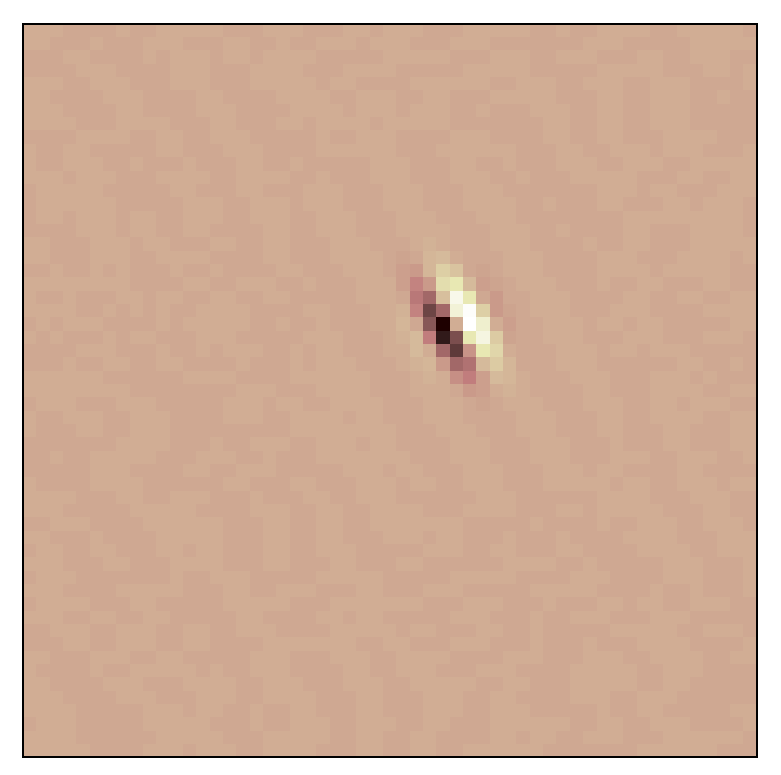
\includegraphics[height=1.8in]{morlet_ima.eps}
					\caption{\centering Imaginary part  of $\psi$.}
				\end{subfigure}%
				~ 
				\begin{subfigure}[t]{0.3\textwidth}
					\centering
					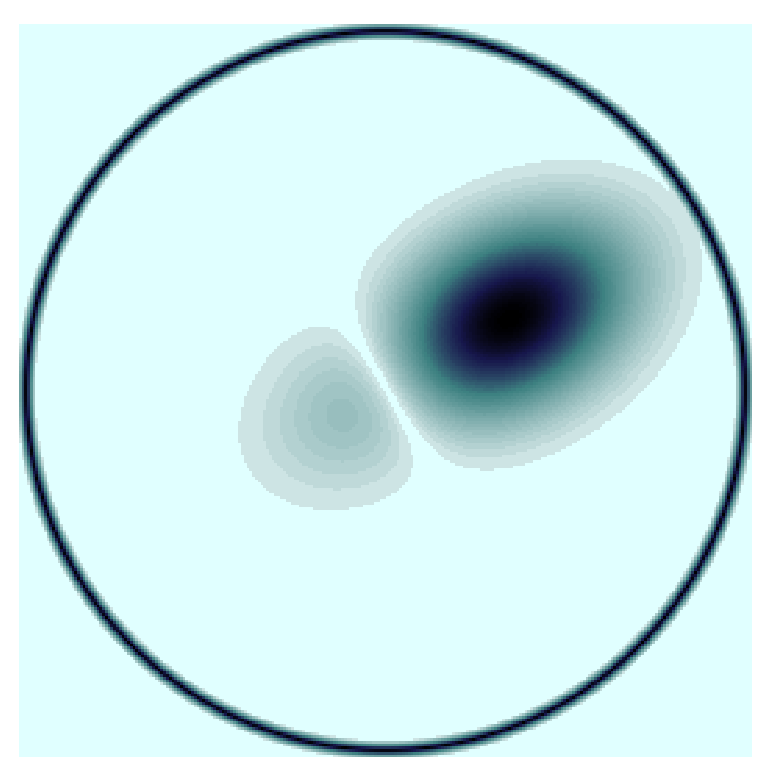
\includegraphics[height=1.8in]{morlet_fourier.eps}
					\caption{\centering Fourier modulus $|\hat{\psi}|i$.}
				\end{subfigure}				
				\caption{Complex Morlet wavelet.}
				\label{fig:Morlet wavelet}
			\end{figure}

      As opposed to the Fourier sinusoidal waves, wavelets are operators stable to local $\mathbf{\mcalL^{2}}$ deformations as they can be expressed as localized waveforms~\citep{mallat1999wavelet}. However, as wavelet transform computes a convolutions with a wavelet basis, the resulting transform is a translation covariant operator~\citep{bruna2013invariant}.\\
        
      To ensure a translation invariant behaviour for an operator initially commuting with translations, one has to introduce a non-linearity in the processing pipeline. Integration is an example of such a non-linearity. Let $R$ be an operator linear or not commuting with translations $L_{c}$, \ie $R(L_{c}\bfx) = L_{c}R(\bfx)$), then the integral $\int R(\bfx(u))du$ is  translation invariant. Applying such a non-linearity to a wavelet transform is equivalent to setting $R(\bfx) = \bfx \ast \psi_{\lambda}$ and one gets the trivial invariant, 
      
      \begin{equation*}
				\label{eq:Trivial invariant}
				\int \bfx \ast \psi_{\lambda}(u)du = 0,
      \end{equation*}
      
      for all signal $\bfx$ because, by definition, $\int \psi_{\lambda}(u)du = 0$.\\
      
      However to preserve the informative character of the scattering operator, one has to ensure a non-vanishing integral. To do so a second operator $M$ has to be introduced such that $M \circ R(\bfx) = M(\bfx \ast \psi_{\lambda})$ has a non-vanishing integral. If $M$ was a linear transformation commuting with translation then the integral would still vanish. Hence one has to choose $M$ among the non-linear operator family.\\
      
      Keeping in mind that the scattering transform has to be stable to deformations, one also imposes on $M$ to commute with deformations, 
      
      \begin{equation*}
				\label{eq:Commute with deformations}
				\forall \tau(u) \; , \; M L_{\tau} = L_{\tau} M.
      \end{equation*}
      
      Adding a weak differentiability condition, one can prove~\citep{bruna2012commute} that $M$ must necessarily be a point-wise operator, \ie $M \circ R(\bfx(u))$ only depends on the value of $\bfx(u)$.\\
      
      Finally, by adding the $\mathbf{\mcalL^{2}}(\dsR^{2})$ stability constraint,
      
      \begin{equation*}
				\label{eq:L2 stability}
				\forall \bfx,\bfx' \in \mathbf{\mcalL^{2}}(\dsR^{2}), \;\;\; 
				\norm{M \circ R(\bfx)} = \norm{\bfx} 
				\;\;\; \text{and} \;\;\;
				\norm{M \circ R(\bfx) - M \circ R(\bfx')} \leq \norm{\bfx-\bfx'},
      \end{equation*}     
      
      one can show~\citep{bruna2012commute} that necessarily,
      
      \begin{equation*}
				M(R(\bfx))= e^{i\alpha}\abs{R(\bfx)}.
				\label{eq:Non-linearity general form}
      \end{equation*}

      The scattering transform is defined using the simplest version of Equation~\ref{eq:Non-linearity general form}. This is $\alpha = 0$ and therefore the resulting coefficients are the $\mathbf{\mcalL^{1}}(\dsR^{2})$ norms,
       
      \begin{equation*}
				\label{eq:L1 norm}
				\norm{\bfx \ast \psi_{\lambda}}_{1} = \int \abs{\bfx \ast \psi_{\lambda}} du
      \end{equation*}      
      
      The family of the $\mathbf{\mcalL^{1}}(\dsR^{2})$ normed wavelet $\{ \norm{\bfx \ast \psi_{\lambda}}_{1}\}_{\lambda}$ generates a crude signal representation which measures the sparsity of the wavelet coefficients. It can be proven that the signal $\bfx$ can be reconstructed from $\{\abs{\bfx \ast \psi_{\lambda}(u)} \}_{\lambda}$ up to a multiplicative constant~\citep{waldspurger2015phase}. This means that the information loss in $\{\norm{\bfx \ast \psi_{\lambda}}_{1} \}_{\lambda}$ occurs during the integration of the absolute value $\abs{\bfx \ast \psi_{\lambda}(u)}$ which removes all non-zero frequencies. However those components can be recovered by calculating the wavelet coefficients $\abs{\bfx \ast \psi_{\lambda_{1}}} \ast \psi_{\lambda_{2}}(u)$ of the new signal $\abs{\bfx \ast \psi_{\lambda_{1}}}$. By doing so their $\mathbf{\mcalL^{1}}(\dsR^{2})$ norms define a much larger family of invariants,
      
      \begin{equation*}
				\label{eq:2nd order}
				\forall (\lambda_{1}, \lambda_{2}) \in (G \times \dsZ) \times (G \times \dsZ) \;\;\; 
				\norm{ \abs{\bfx \ast \psi_{\lambda_{1}}} \ast \lambda_{2}}_{1} =
				\int \abs{ \abs{\bfx \ast \psi_{\lambda_{1}}(u)} \ast \psi_{\lambda_{2}}} du.
      \end{equation*}          
      
      By further iterating on the wavelet/modulus operators, more translation invariant coefficients can be generated. The building bloc of such a model ---the scattering propagator--- is thus the absolute value of the convolution between a wavelet and the input signal.
      
      \begin{defn} \textbf{(Scattering propagator)}\\ 
				The scattering operator $U$ for a scale and an orientation $\lambda \in G \times \dsZ$ is defined as the absolute value of the input convolved with the wavelet operator at this scale and orientation.
				
				\begin{equation}
					\label{eq:scattering propagator}
					U[\lambda](\bfx) \eqdef \abs{\bfx \ast \psi_{\lambda}}.
				\end{equation}
				\label{def:SO}
			\end{defn}
						
			\begin{defn} \textbf{(Path ordered scattering propagators)}\\ 
				Any sequence $p = (\lambda_{1}, \lambda_{2},\dots ,\lambda_{m})$ where $\forall i \in \llbracket 1,m \rrbracket \;\; \lambda_{i} \in G \times \dsZ$ defines a path of length $m$, \ie the ordered product of non-linear and non-commuting operators,
				
				\begin{equation}
					\label{eq:path ordered SP}
					\begin{split}
						U[p]\bfx &\eqdef U[\lambda_{m}]\dots U[\lambda_{2}]U[\lambda_{1}](\bfx) \\
							&= \abs{\abs{\abs{\abs{\bfx \ast \psi_{\lambda_{1}}} \ast \psi_{\lambda_{2}}} 
							\dots } \ast \psi_{\lambda_{m}}}.   
					\end{split}
				\end{equation}
				
				With the convention: $U[\emptyset]\bfx = \bfx$.\\
				\label{def:path ordered SO}
      \end{defn} 
      
      This propagator can be used to provide a first formal definition of the scattering coefficients.
      
      \begin{defn} \textbf{(Scattering coefficient)}\\
				A scattering coefficient along the path $p$ is defined as an integral of the $p$ ordered scattering propagators, normalized by the response of a Dirac:

				\begin{equation}
					\label{eq:ST1}
					\bar{S}[p](\bfx) \eqdef \mu_{p}^{-1} \int U[p]\bfx(u) du,
				\end{equation}
				
				with,
				
				\begin{equation*}
					\label{eq:ST normalization}
					\mu_{p} \eqdef \int U[p]\delta(u)du.      
				\end{equation*}
				\label{def:SC}
      \end{defn}
      
      Section~\ref{sec:ST/Pties} shows that each scattering coefficient $\bar{S}[p](\bfx)$ is ---as desired--- invariant to translation of the input $\bfx$ and Lipschitz continuous to deformations. But for prediction tasks, one might want to compute localized descriptors only invariant to translations smaller than a predefined scale $2^{J}$, while keeping the spatial variability at scales larger than $2^{J}$. This can be achieved by localizing the scattering integral with a scaled spatial window $\phi_{2^{J}}(u) = 2^{-2J} \phi(2^{-2J}u)$. This yields the definition of the windowed scattering transform.
      
      \begin{defn} \textbf{(-Windowed- scattering coefficient of order $m$)}\\
				If $p$ is a path of length $m \in \mathds{N}$, the ---windowed--- scattering coefficient of order $m$ localized at scale $2^{J}$ ($J \in \dsN$) is defined as:
				
				\begin{equation}
					\label{eq:ST windowed}
					\begin{split}
						S_{J}[p](\bfx) &\eqdef U[p]\bfx \ast \phi_{2^{J}}(u) \\
									&= \int U[p]\bfx(v) \phi_{2^{J}}(u-v) dv \\
									&= \abs{\abs{\abs{\abs{\bfx \ast \psi_{\lambda_{1}}} \ast \psi_{\lambda_{2}}} 
							\dots } \ast \psi_{\lambda_{m}}} \ast \phi_{2^{J}}(u),
					\end{split}
				\end{equation}
				
				With the convention: $S_{J}[\emptyset]\bfx = \bfx \ast \phi_{2^{J}}$.\\
      	\label{def:SC windozed}
      \end{defn}

		\section{Scattering Convolution Network:}
			\label{sec:ST/SCN}
			
			This section introduces the scattering transform as an iterative process over a one-step operator and creates a parallel with convolutional neural networks~\citep{lecun2010convolutional}.\\
			
			For $J \in \dsN^{\ast}$, let $U_{J}[\Omega] \eqdef \{U_{J}[p]\}_{p \in \Omega}$ and $S_{J}[\Omega] \eqdef \{S_{J}[p]\}_{p \in \Omega}$. They defines families of operators indexed by a set of paths $\Omega$. One can compute a windowed scattering transform by iterating over the one-step ---windowed--- propagator $U_{J}$.
			
			\begin{defn}  \textbf{(Scattering one-step propagator)}\\
				The one-step propagator $\mcalU_{J}$ can be defined as,
				\begin{equation}
					\forall \bfx \in \mcalL^{2}(\dsR^{d}) \;\;\;
					\mcalU_{J} \bfx = \{ A_{J}\bfx , \; (U[\lambda]\bfx)_{\lambda \in \Lambda_{J}} \},
					\label{eq:One step propagator}
				\end{equation}
				
				where $A_{J}\bfx = \bfx \ast \phi_{2J}$, $U[\lambda]\bfx = \abs{\bfx \ast \psi_{\lambda}}$ and $\Lambda_{J} = G \times \llbracket0, J \rrbracket$.\\
				\label{def:One step propagator}
			\end{defn}
			
			After calculating $\mcalU_{J}\bfx$, applying $\mcalU_{J}$ again to each $U[\lambda]\bf$ generates a larger infinite family of functions. And since, for all path $p$, $U[\lambda_{2}]U[p] = U[p+\lambda_{2}]$ and $ A_{J}U[p] = S_{J}[p]$; it holds that,
			
			\begin{equation}
					\forall \bfx \in \mcalL^{2}(\dsR^{d}) \;\;\; \mcalU_{J}U[p] \bfx = \{ S_{J}[p]\bfx , \; (U[p+\lambda_{2}]\bfx)_{\lambda_{2} \in \Lambda_{J}} \},
					\label{eq:SCN propagation 1}
			\end{equation}\\
			
			Let now $\Lambda_{J}^{m}$ denotes the set of all paths of length $m$ with the convention $\Lambda_{J}^{0} = \{ \emptyset \}$, its propagation is,
			
			\begin{equation}
					\forall \bfx \in \mcalL^{2}(\dsR^{d}) \;\;\; \mcalU_{J}U[\Lambda_{J}^{m}] \bfx = \{ S_{J}[\Lambda_{J}^{m}]\bfx , \; (U[\Lambda_{J}^{m+1}]\bfx)_{\lambda \in \Lambda_{J}} \}.
					\label{eq:SCN propagation 2}
			\end{equation}\\
			
			\begin{defn}  \textbf{(Scattering transform)}\\			  
			  The scattering transform of order $m$ at scale $J$ can be defined as the set of scattering coefficients obtained for all paths of length $0$ to $m$,
			  \begin{equation}
			    S_{J}[\mcalP_{J}^{m}]\bfx = \big[S_{J}[\Lambda_{J}^{0}]\bfx , \dots , S_{J}[\Lambda_{J}^{m}]\bfx \big].\\
					\label{eq:scattering transform}
			  \end{equation}\\ 
			\end{defn}
			
			Hence the scattering transform of infinite depth $S_{J}[\mcalP_{J}]\bfx$ can be computed from $\bfx= U[\emptyset]\bfx$ by iteratively computing $\mcalU_{J}U[\Lambda_{J}^{m}] \bfx$ for $m$ going from $1$ to $\infty$. This iterative process is illustrated in Figure~\ref{fig:SCN}.\\
			
			One can notice that the scattering calculation as the same general architecture as the convolutional neural networks introduced by~\citet{lecun1995convolutional}. Both CNN and Scattering Convolutional Network (SCN) cascade a convolution step and a ``pooling'' non linearity. However while convolutional neural networks use kernel filters learned from the data with back-propagation algorithm, SCNs use a fixed wavelet filter bank. 
			%TODO: more on the topic from the roto translation paper

      \begin{figure}[h]
				\begin{center}
					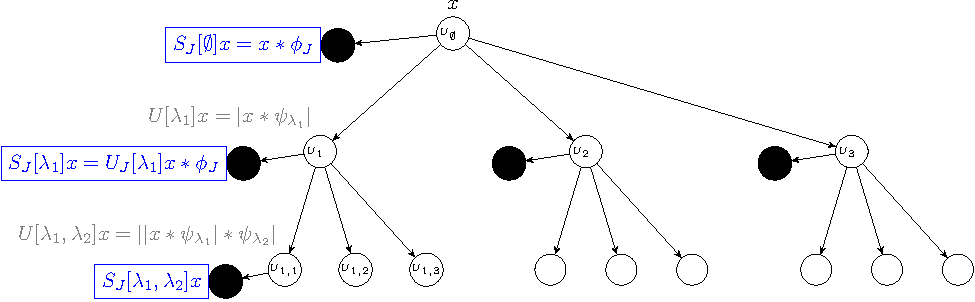
\includegraphics[width=5in]{ST_crop.pdf}
					\caption[Scattering convolutional network architecture.]{\centering A scattering propagator $U_{J}$ applied to a signal $\bfx$ computes each $U[\lambda_{i}]\bfx = |\bfx \ast \psi_{\lambda_{i}}|$ and outputs $S[\emptyset]\bfx= \bfx \ast \phi_{2^{J}}$. Applying $U_{J}$ to each  $U[\lambda_{i}]\bfx$ computes all $U[\lambda_{i},\lambda_{j}]\bfx$ and outputs $S_{j}[\lambda_{i}] =  U[\lambda_{i}] \ast \phi_{2^{J}}$. Applying iteratively $U_{J}$ to each $U[p]\bfx$ outputs $S_{J}[p]\bfx = U[p]\bfx \ast \phi_{2^{J}}$ and computes the next path layer.}
					\label{fig:SCN}
				\end{center}	
      \end{figure}
      
      
      
	\section{Properties of the scattering transform:}
		\label{sec:ST/Pties}
		
		The scattering coefficient having been defined, one can be interested in the characteristics of such a data representation. This section provides an overview of some of the properties of the scattering transform. It also introduces an approximation to the scattering convolution network defined in the previous section, leading to computationally tractable networks.\\
		
		\begin{note}
		  Formal proofs for most of those properties can be found in~\citep{mallat2012gis}.
		\end{note}

		\subsection{Non-expansivity:}
			\label{subsec:ST/Pties/Non-expansivity}
			The scattering one-step propagator,
			
			\begin{equation*}
			  \mcalU_{J} \bfx = \{ A_{J}\bfx , \; (U[\lambda]\bfx)_{\lambda \in \Lambda_{J}} \} = \{ A_{J}\bfx , \; (\abs{W_{J}\bfx})_{\lambda \in \Lambda_{J}} \},
				\label{eq:One step propagator 2}
			\end{equation*}

			results of the composition of a wavelet transform $W_{J}$ that is unitary and of a modulus operator that is non-expansive ---as $\forall (a,b) \in \dsC^{2} \abs{\abs{a}-\abs{b}} \leq \abs{a-b}$--- and is thus also non-expansive. Since the scattering transform $S_{J}[\mcalP_{J}]$ iterates on $\mcalU_{J}$, the proposition (proof adapted from~\citep{lohmiller1998contraction}) proves that $S_{J}[\mcalP_{J}]$ is also non-expansive.
			
			\begin{prop} \textbf{(Non-expansive)}\\ 
				The scattering transform is non expansive.
				\begin{equation}
				  \forall \bfx,\bfx' \in \mcalL^{2}(\dsR^{d}) \;\;\; \norm{S_{J}[\mcalP_{J}]\bfx - S_{J}[\mcalP_{J}]\bfx'} \leq \norm{\bfx-\bfx'}
  			  \label{eq:Nonexpansivity}
				\end{equation}
			  \label{pty:Nonexpansivity}
			\end{prop}

		\subsection{Energy preservation:}
			\label{subsec:ST/Pties/Energy}
			Each scattering propagator $U[\lambda]\bfx = \abs{\bfx \ast \psi_{\lambda}}$ captures the frequency energy contained in the signal $\bfx$ over a frequency band covered by the Fourier transform $\hat{\psi}_{\lambda}$ and propagates this energy towards lower frequencies. It can thus be proved that under some assumptions on the wavelet ---admissible wavelet, the whole scattering energy ultimately reaches the minimum frequency $2^{-J}$ and is trapped by the low-pass filter $\phi_{2^{J}}$. Thus the energy propagated by a ---windowed--- scattering transform goes to $0$ as the path length increases, implying that $\norm{S_{J}[\mcalP_{J}]} = \norm{x}$\\
			
			But prior to showing this, one must states the necessary assumptions to be made on the wavelet used.
						
			\begin{note}
			  The notation $\hat{(.)}$ is used to design the Fourier transform.
			\end{note}

						
			\begin{defn} \textbf{(Admissible scattering wavelet)}\\ 
				A scattering wavelet $\psi$ is admissible if there exist $\eta \in \dsR^{d}$ and $\rho \in \mcalL^{2}(\dsR^{d})$ positive, with $\abs{\hat{\rho}(\omega)} \leq \abs{\hat{\phi}(2\omega)}$ and $\hat{\rho}(\omega)=0$, such that the function,
				
				\begin{equation}
					\hat{\Psi}(\omega) = \abs{\hat{\rho}(\omega - \eta)}^{2} - \sum_{k=1}^{+\infty}k(1-\abs{\hat{\rho}(2^{-k}(\omega - \eta)}^{2}),
				\end{equation}
				
				satisfies,
				
				\begin{equation}
				  \alpha = \inf_{1 \leq \abs{\omega}\leq 2} \sum_{j=-\infty}^{+\infty}\sum_{r \in G} \hat{\Psi}(2^{-j}r^{-1}\omega) \abs{\hat{\psi}(2^{-j}r^{-1}\omega)}^{2} > 0.\\
				\end{equation}
				
				\label{def:Admissible wavelet}
			\end{defn}

			For an admissible wavelet one can prove that the scattering transform conserves the energy of the signal.
			
			\begin{thm} \textbf{(Energy conservation)}\\ 
				If the scattering wavelet $\psi$ is admissible, then for all signal $\bfx \in \mcalL^{2}(\dsR^{d})$,
				
				\begin{equation}
				  \lim_{m \rightarrow +\infty} \norm{U[\Lambda_{J}^{m}]\bfx}^{2} = \lim_{m \rightarrow +\infty} \sum_{n=m}^{+\infty} \norm{S_{J}[\Lambda_{J}^{n}]\bfx}^{2} = 0,
					\label{eq:energy conservation 1}
				\end{equation}
				
				and
				
				\begin{equation}
				  \norm{S_{J}[P_{J}]\bfx}^{2} = \norm{\bfx}.
				  \label{eq:energy conservation 2}
				\end{equation}
				\label{thm:Energy conservation}
			\end{thm}

			The proof of the Theorem~\ref{thm:Energy conservation} also shows that the scattering energy propagates progressively towards lower frequencies and that the energy of $U[p]\bfx$ is mainly concentrated along frequency decreasing paths $p=(\lambda_{k})_{k\leq m}$, \ie for which $\abs{\lambda_{k+1}} \leq \abs{\lambda_{k}}$. The energy contained in the other paths is negligible and thus for the applications in this document only frequency decreasing paths are considered.\\
			
			Moreover, the decay of $\sum_{n=m}^{+\infty} \norm{S_{J}[\Lambda_{J}^{n}]x}^{2}$ implies that there exist a path length $M > 0$ after which all longer paths can be neglected. For signal processing applications, this decay appears to be exponential. And for classification applications, paths of length $M = 3$ provides the most interesting results~\citep{anden2011multiscale},~\citep{bruna2010classification}.\\
			
			The restrictions stated above yield an easier parametrization of a scattering network. Indeed when only the frequency decreasing paths up to a given order are considered, a scattering network is completely defined by:\\
			\begin{itemize}
				\item $\psi$: The admissible wavelet used. In the remainder of the document, unless stated otherwise, the Morlet wavelet is used.
			  \item $M$: The maximum path length considered.
			  \item $J$: The finest scale level considered.
			  \item $L$: The number of orientation considered, which can be defined as the cardinality of the previously define ensemble $G$.\\
			\end{itemize}
			
			Hence for a given set of parameter $(\psi, M,J,L)$, one can generate one and only one frequency decreasing paths scattering network. Let $ST_{(\psi, M,J,L)}(\bfx)$ now denotes the frequency decreasing windowed scattering convolutional network of parameter $(\psi, M,J,L)$ evaluated for signal $\bfx$. Each node $i$ of this network generates a -possibly empty- set of of nodes of size $(j_{i}-1) \times L$ where $j_{i}$ is the scale of node $i$ and $L$ is the number of orientations considered. Finally the number of nodes $O$ of this network is,
			
			\begin{equation}
			  O = \sum_{m=0}^{M-1} \binom{J}{m} . L^{m}
			  \label{eq:ST number of node}
			\end{equation}

			and it has the architecture displayed by Figure~\ref{fig:SCN 2}. 
			
			\begin{figure}[h]
				\begin{center}
					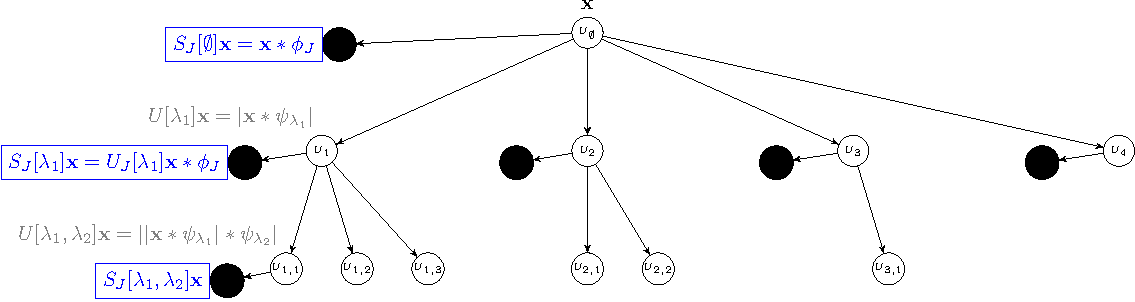
\includegraphics[width=5in]{ST_freqDec_crop.pdf}
					\caption[Frequency decreasing scattering convolution network.]{\centering  Frequency decreasing scattering convolution network with $J=4$, $L=1$ and $M=2$. A node $i$ at scale $j_{i}$ generates $(j_{i}-1) \times L$ nodes. }
					\label{fig:SCN 2}
				\end{center}	
      \end{figure}
      
		\subsection{Translation invariance:}
			\label{subsec:ST/Pties/Translation}		
			The translation invariance of the scattering transform $S_{J}[\mcalP_{J}]$ can be proved for a limit metric when $J$ goes to infinity. To do so one can first prove that the scattering distance $\norm{S_{J}[\mcalP_{J}]\bfx - S_{J}[\mcalP_{J}]\bfx'}$ converges when $J$ goes to infinity --- as it is non-increasing when $J$ increases (see section~\ref{subsec:ST/Pties/Non-expansivity}). From there one can bound the distance between the scattering transform of the signal and the one of its translated version $\norm{S_{J}[\mcalP_{J}]\mcalL_{c}\bfx - S_{J}[\mcalP_{J}]\bfx}$ and prove that this bound tends to $0$ when $J$ goes to infinity. This proves the translation invariance.
			
			\begin{thm} \textbf{(Translation invariance)}\\
				For admissible scattering wavelets,
				
				\begin{equation}
					\forall \bfx \in \mcalL^{2}(\dsR^{d}), \; \forall c \in \dsR^{d} \;\;\; \lim_{J \rightarrow \infty} \norm{S_{J}[\mcalP_{J}]\mcalL_{c}\bfx - S_{J}[\mcalP_{J}]\bfx} = 0
					\label{eq:Tranlation invariance}
				\end{equation}
				\label{thm:Translation invariance}
			  
			\end{thm}

		\subsection{Lipschitz continuity to the action of diffeomorphisms:}
			\label{subsec:ST/Pties/Lipschitz continuity}			
			The Lipschitz continuity to the action of diffeomorphisms of $\dsR^{d}$ can be proved for deformations sufficiently close to translations. Such diffeomorphisms map $u$ to $u-\tau(u)$ where $\tau(u)$ is a displacement filed such that $\norm{\nabla \tau}_{\infty} < 1$ ---\ie invertible transformations~\citep{bruna2013invariant}. Let $L_{\tau}\bfx(u)=\bfx(u-\tau(u))$ denotes the action of such diffeomorphisms on the signal $\bfx$. Once again, one can find an upper bound to the distance between the scattering transform of the signal and the one of its deformed version $\norm{S_{J}[\mcalP_{J}]\mcalL_{\tau}\bfx - S_{J}[\mcalP_{J}]\bfx}$. With a bit of work on this bound, one can then proved that the consequences of the action of $L_{\tau}$ is bounded by a translation term proportional to $2^{-J} \norm{\tau}_{\infty}$ and a deformation error proportional to $\norm{\nabla \tau}_{\infty}$. Finally some more work on the bounding term provides the Lipschitz continuity.
			
			\begin{thm} \textbf{(Lipschitz continuity to the action of diffeomorphisms)} \\
			  There exists $C$ such that all $\bfx \in \mcalL(\dsR^{d})$ with $\norm{U[\mcalP_{J}]\bfx}_{1} < \infty$ and all $\tau \in \mcalC^{2}(\dsR^{d})$ with $\norm{\nabla \tau}_{\infty} < \frac{1}{2}$ satisfy,
			  
			  \begin{equation}
					\norm{S_{J}[\mcalP_{J}]\mcalL_{\tau}\bfx - S_{J}[\mcalP_{J}]\bfx + \tau . \nabla S_{J}[\mcalP_{J}]\bfx} \leq C \norm{U[\mcalP_{J}]\bfx}_{1} K(\tau),
					\label{eq:Lipschitz continuity 1}
			  \end{equation}

			  with
			  
			  \begin{equation}
					K(\tau) = 2^{-2J} \norm{\tau}_{\infty}^{2} + \norm{\nabla \tau}_{\infty} \left(\max \left( \log \frac{\norm{\Delta \tau}_{\infty}}{\norm{\nabla \tau}_{\infty}},1 \right) \right) + \norm{H\tau}_{\infty}.
					\label{eq:Lipschitz continuity K(tau)}
			  \end{equation}
			  \label{thm:Lipschitz continuity}
			\end{thm}
			
			\begin{rem}
				If the case where $2^{J} \gg \norm{\tau}_{\infty}$ and $\norm{\nabla \tau}_{\infty} + \norm{H \tau}_{\infty} \ll 1$, then $K(\tau)$ becomes negligible and the displacement field $\tau(u)$ can be estimated at each $u \in \dsR^{d}$. This can be done by solving the linear equation resulting from Equation~\ref{eq:Lipschitz continuity 1} under the assumptions mentioned above,
				
				\begin{equation}
					\forall p \in \mcalP_{J} \norm{S_{J}[p]\mcalL_{\tau}\bfx - S_{J}[p]\bfx + \tau . \nabla S_{J}[p]\bfx} \approx 0.
					\label{eq:Lipschitz continuity 2}  
				\end{equation}
				
				This estimate of the displacement field can be used for many applications such as object tracking in video sequences or image sequence restoration~\citep{brailean1996recursive}.
			\end{rem}
			
		
  \section{Application to classification:}
    \label{sec:ST/Applications to clf}
   
    The scattering transform maps a given realisation of a high-dimensional signal into an even higher-dimensional space where the classification task is simplified due to the inherent properties described in the previous section yielding easily separable data clusters in the ``scattering'' space.\\
    
    The scattering transform has been successfully applied in classification of a wild variety of signals such as audio signals~\citep{anden2011multiscale}, images~\citep{oyallon2014deep} or electrocardiograms~\citep{chudacek2014low} and in the vast majority ---if not all--- the classification task has been done using the features generated by the transform of the dataset as inputs for a discriminative classifier, e.g. Support Vector Machine classifier. The new input vector is obtained by concatenating the scattering coefficients of all orders, scale and orientations into a unique $1$-D vector -for 2-D signal the scattering coefficients are also flattened. Leveraging the richness of the representation generated the scattering transform combined to an SVM classifier provides performance comparable to those of a -small- deep convolutional neural network~\citep{oyallon2013generic}. This section proposes to test this framework on the handwritten digit dataset \textit{MNIST}.\\
    
    \textit{MNIST} is composed of $28 \times 28$ binary and centred images of handwritten digits. The dataset is split into a training set of $50000$ images and a testing set of $10000$ images and the task at hand is a $10$ classes classification problem.\\
    
		\begin{figure}[h]
			\centering
			\begin{subfigure}[t]{0.17\textwidth}
				\centering
				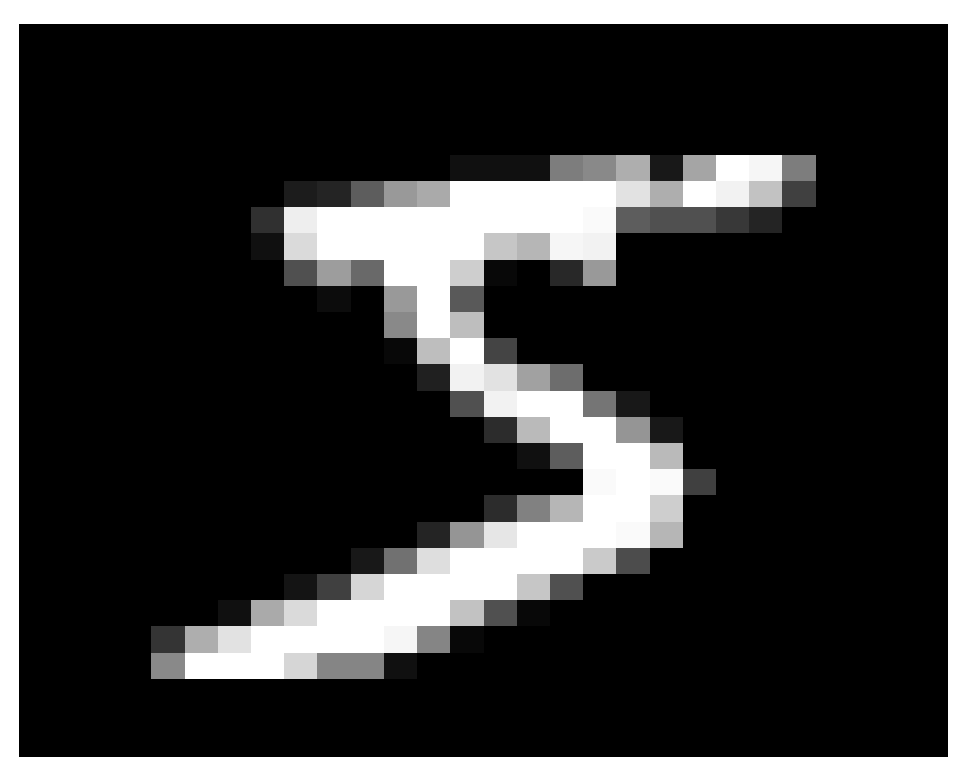
\includegraphics[height=0.9in]{mnist_1.eps}
			\end{subfigure}%
			~ 
			\begin{subfigure}[t]{0.17\textwidth}
        \centering
        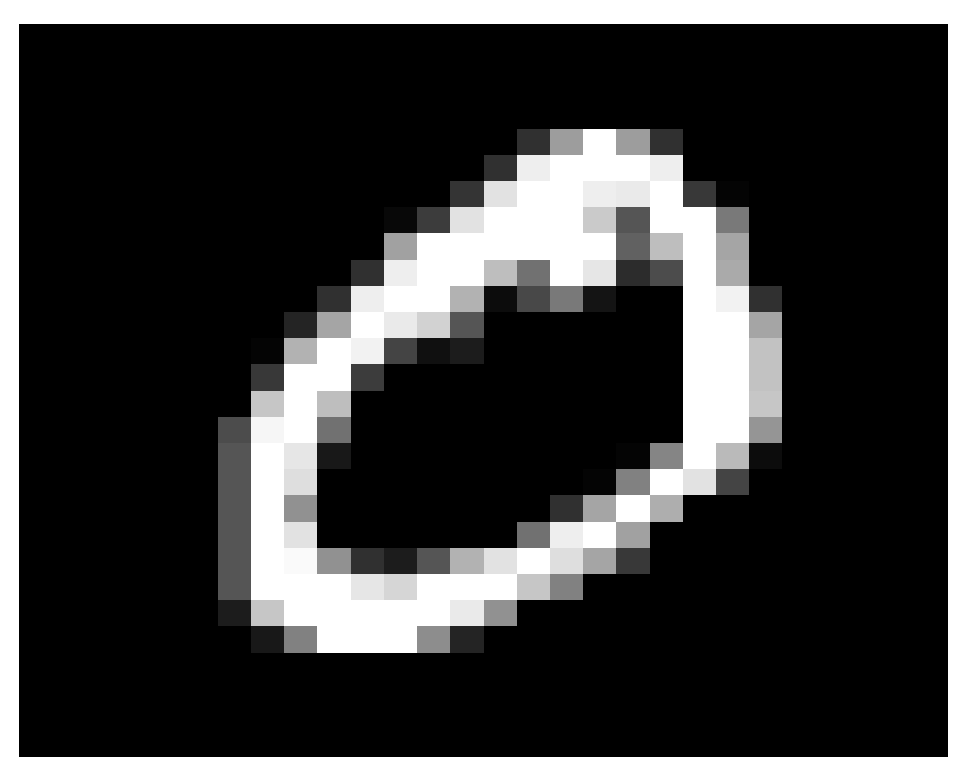
\includegraphics[height=0.9in]{mnist_2.eps}
			\end{subfigure}
			~ 
			\begin{subfigure}[t]{0.17\textwidth}
        \centering
        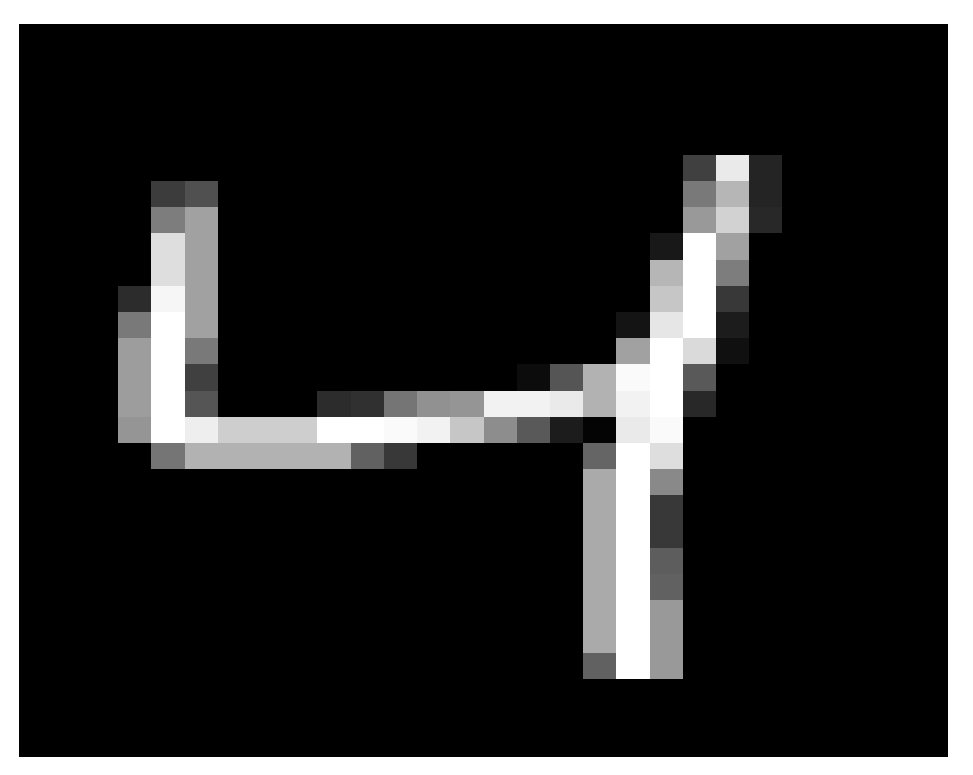
\includegraphics[height=0.9in]{mnist_3.eps}
			\end{subfigure}
			~ 
			\begin{subfigure}[t]{0.17\textwidth}
        \centering
        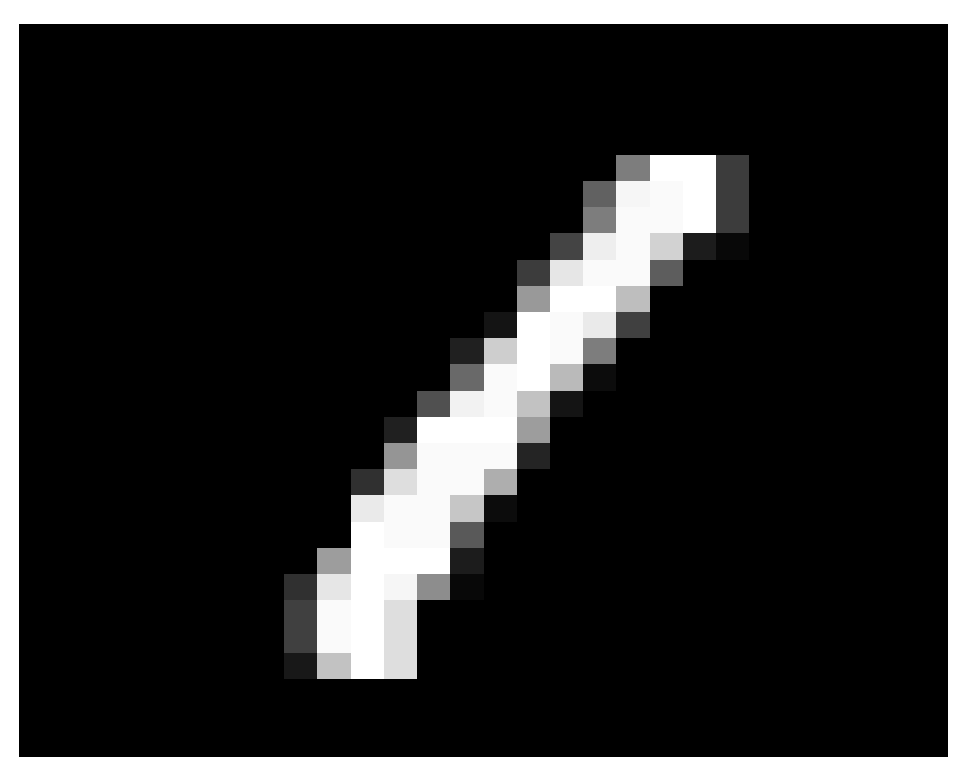
\includegraphics[height=0.9in]{mnist_4.eps}
			\end{subfigure}
			~ 
			\begin{subfigure}[t]{0.17\textwidth}
        \centering
        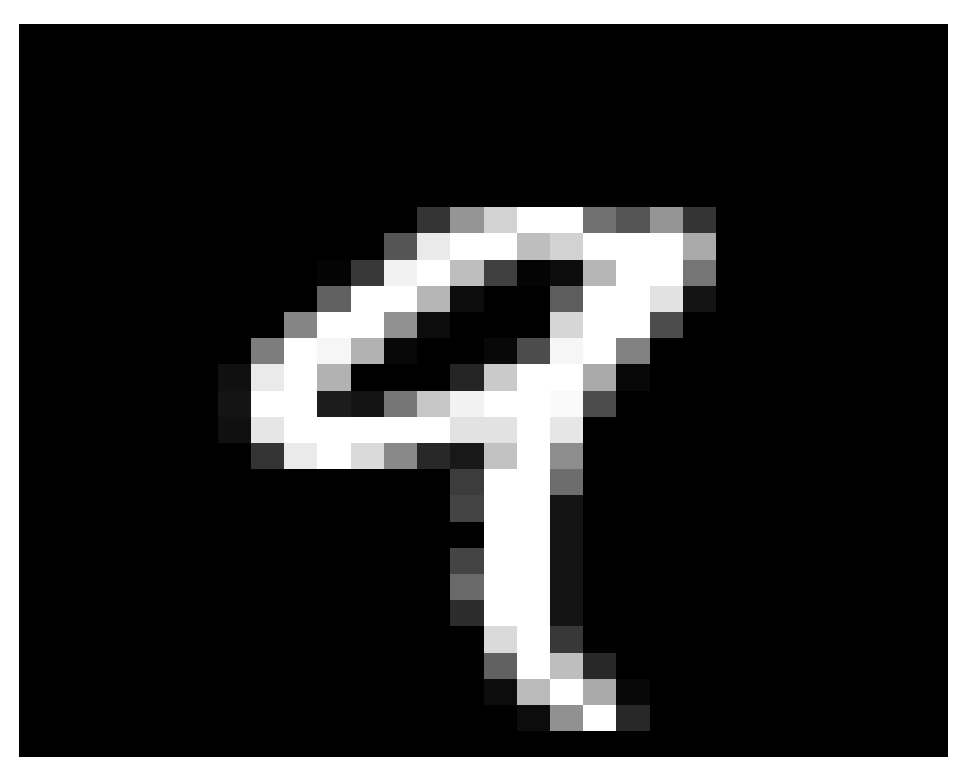
\includegraphics[height=0.9in]{mnist_5.eps}
			\end{subfigure}
			\\
			~
			\begin{subfigure}[t]{0.17\textwidth}
				\centering
				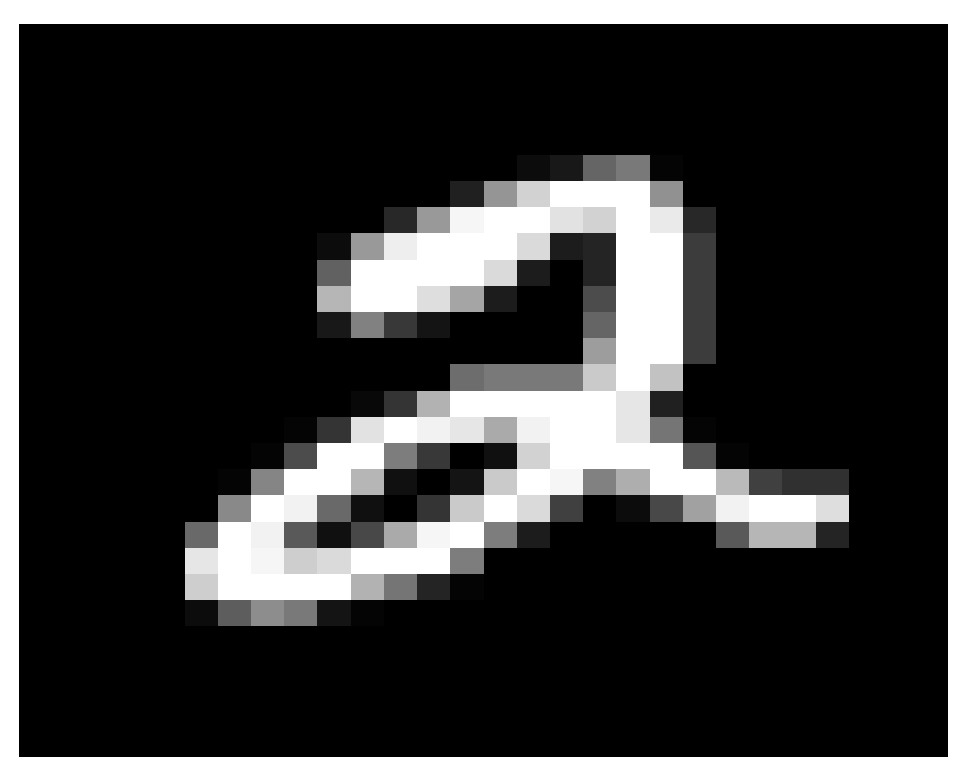
\includegraphics[height=0.9in]{mnist_6.eps}
			\end{subfigure}%
			~ 
			\begin{subfigure}[t]{0.17\textwidth}
        \centering
        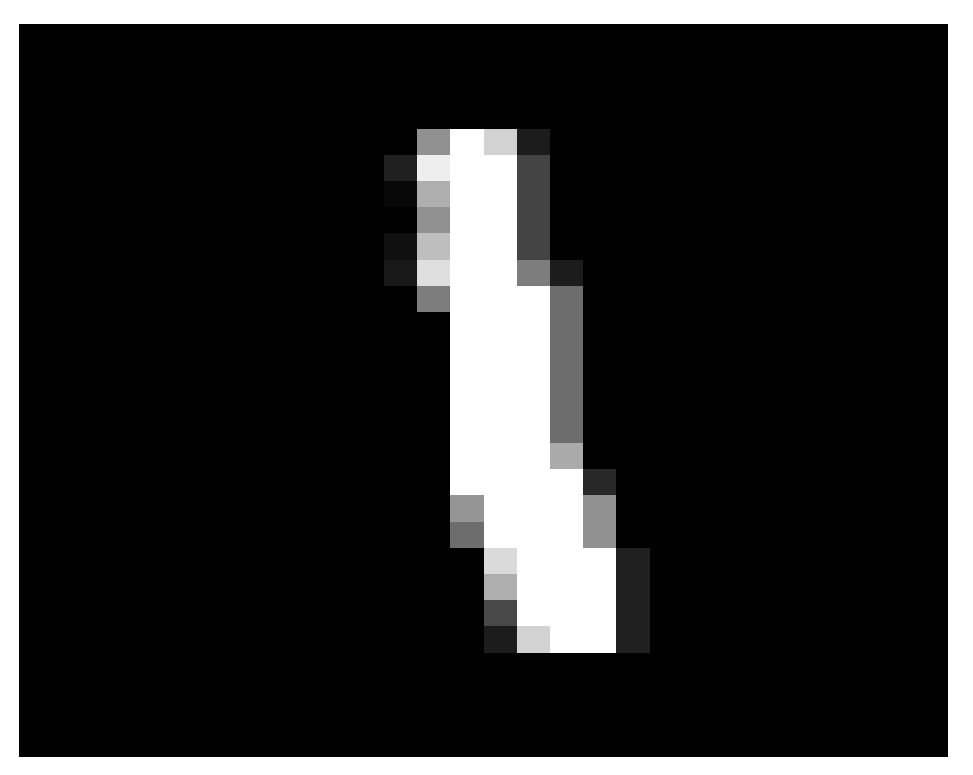
\includegraphics[height=0.9in]{mnist_7.eps}
			\end{subfigure}
			~ 
			\begin{subfigure}[t]{0.17\textwidth}
        \centering
        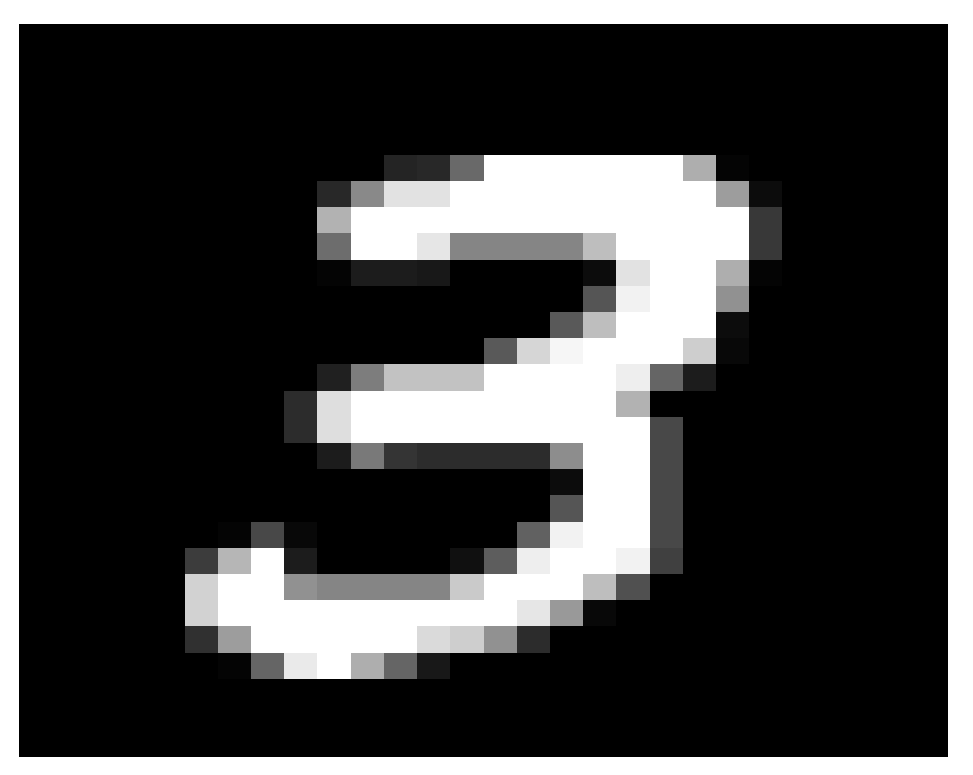
\includegraphics[height=0.9in]{mnist_8.eps}
			\end{subfigure}
			~ 
			\begin{subfigure}[t]{0.17\textwidth}
        \centering
        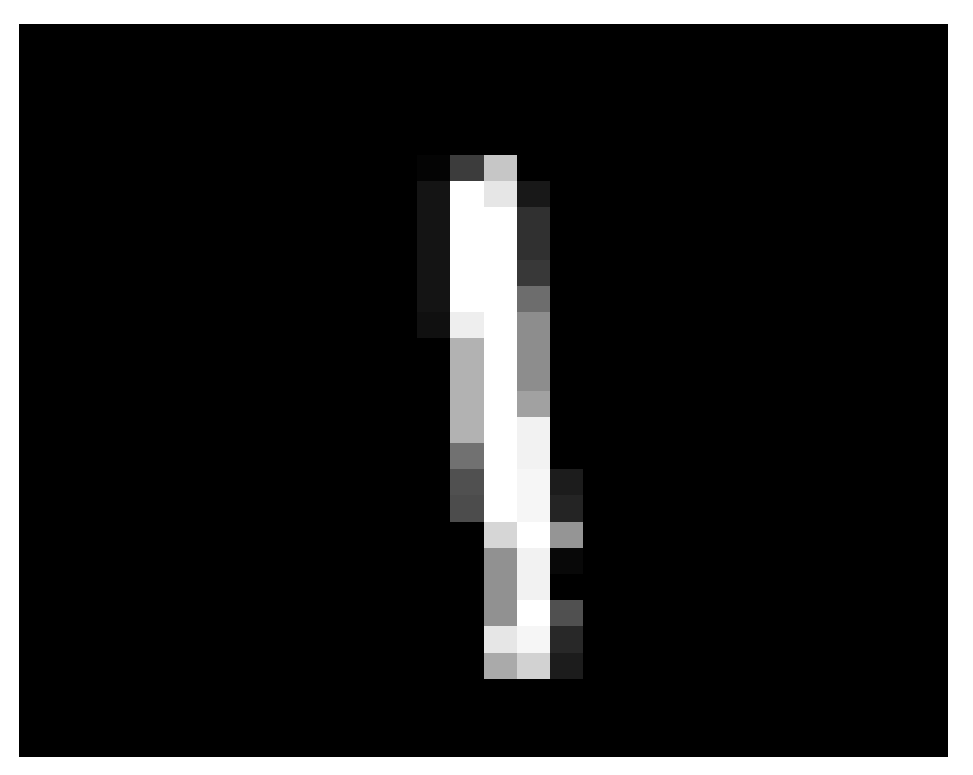
\includegraphics[height=0.9in]{mnist_9.eps}
			\end{subfigure}
			~ 
			\begin{subfigure}[t]{0.17\textwidth}
        \centering
        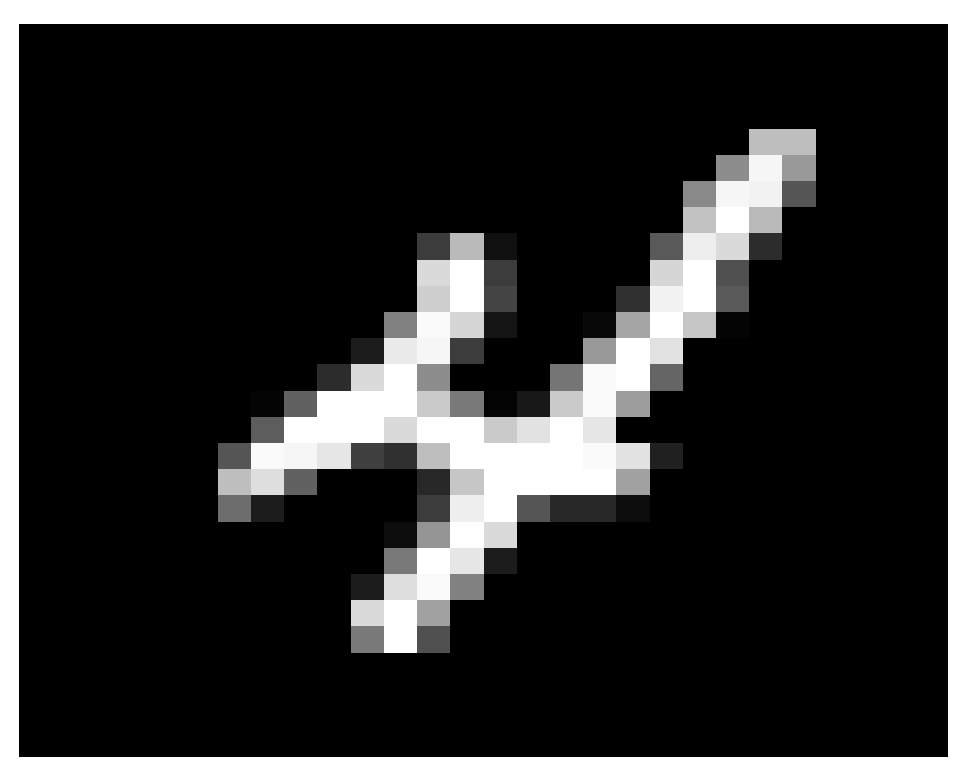
\includegraphics[height=0.9in]{mnist_10.eps}
			\end{subfigure}
			~
			\caption{Samples from MNIST.}
			\label{fig:Mnist}
		\end{figure}
		
		For this task the frequency decreasing scattering convolutional network has $M=3$ layers, breaking down the images into $J=3$ scales and $L=6$ orientations. For each input image this networks generates $127$ scattering coefficients (see Equation~\ref{eq:ST number of node}) and thus yields a $99568$ dimensional feature vector ($127 \times 28 \times 28$). The discriminative classifier used is a set of binary SVM classifiers with a Gaussian radial basis function kernel~\citep{scholkopf1997comparing}. This classifier have two meta-parameters. $\gamma$ defines how influential a single training example is and $C$ the trade off between misclassification of training examples and simplicity of the decision surface. Those meta-parameters are fine-tuned by cross-validation to $C = 3$ and $\gamma = 0.0018$.\\
		
		Using this set-up, the trained model scores $99.47\%$ accuracy on the test set, \ie $9947$ true positive out of $10000$ realisations. This accuracy is of the same order of what can be obtained using a convolutional neural network~\citep{jarrett2009best}~\citep{lecun2015web}.\\
		
		This approach of classification have been used successfully for many more applications but unfortunately it does not directly leverage the structure created by the scattering transform and the possible information contained into it. Nor that it provides a generative models of the data, with all the advantages encompassed (see Section~\ref{sec:Intro/Discr vs gen}). The remainder of this document focuses on building a generative model describing 1a scattering convolutional network.
    
    
%%%%%%%%%%%%%%%%%%%%%%%%%%%%%%%%%%%%%%%%%%%%%%%%%%%%%%%%%%%%%%%%%%%%%%%%%%%%%%%%%%%%%%%%%%%%%%%%%%%%%%%%%%%%%%%%%%%%%%%%%%%%%%%%%%%%%%%%%%%%%%%%%%%%%%%%%%%%%%%%%%%%%%%%%%%%%%%%%%%%%%%%%%%%%%%%%%%%%%%%%%%%%%%%%%%%%%%%%%%%%
%%%%%%%%%%%%%%%%%%%%%%%%%%%%%%%%%%%%%%%%%%%%%%%%%%%%%%%%%%%%%%%%%%%%%%%%%%%%%%%%%%%%%%%%%%%%%%%%%%%%%%%%%%%%%%%%%%%%%%%%%%%%%%%%%%%%%%%%%%%%%%%%%%%%%%%%%%%%%%%%%%%%%%%%%%%%%%%%%%%%%%%%%%%%%%%%%%%%%%%%%%%%%%%%%%%%%%%%%%%%%
%%%%%%%%%%%%%%%%%%%%%%%%%%%%%%%%%%%%%%%%%%%%%%%%%%%%%%%%%%%%%%%%%%%%%%%%%%%%%%%%%%%%%%%%%%%%%%%%%%%%%%%%%%%%%%%%%%%%%%%%%%%%%%%%%%%%%%%%%%%%%%%%%%%%%%%%%%%%%%%%%%%%%%%%%%%%%%%%%%%%%%%%%%%%%%%%%%%%%%%%%%%%%%%%%%%%%%%%%%%%%
\chapter{Probabilistic graphical models:}
  \label{chap:PGMs}
  
  Probabilistic Graphical Models (PGMs) offer an efficient framework to express joint distributions and conditional dependencies. They rely on the usage of a graph based representation of conditional dependence between a set of random variables. Such a graph can then be used to encode a complete distribution over a multi-dimensional space in a compact ---or factorized--- manner. Probabilistic graphical models exist under many forms but they can be split into two main families, the Bayesian Networks (BNs) and the Markov models (MMs). Both families encompass the properties of factorization and independences defined by the graph, but differ when it comes to the specificities of the set of independences they can encode as well as the factorization of the distribution that they can induce~\citep{bishop2006pattern}.\\
  
  Before using a graphical model to describe the scattering transform (see Section~\ref{chap:SCHMT}) this report provides an introduction to PGMs. Note however that the aim of this section is not to present a complete overview of the probabilistic graphical models but rather to introduce some interesting concepts that are used in the remainder of the document either in Section~\ref{chap:SCHMT} to define the scattering convolutional hidden Markov tree or may be mentioned in the Section~\ref{chap:ccl} as possible leads for future work. A reader further interested in PGMs could refer to~\citep{heckerman1998tutorial} or~\citep{bishop2006pattern} for a more complete introduction to those models.\\
  
  This chapter introduces the two main classes of probabilistic graphical models. Section~\ref{sec:PGMs/BN} focuses on the Bayesian networks, while Section~\ref{sec:PGMs/MM} provides more details about Markov models.
	
  \section{Bayesian Networks:}  
    \label{sec:PGMs/BN}
    
    A BN is subclass of probabilistic graphical model where the set of random variables and their conditional dependencies are expressed via a Directed Acyclic Graph (DAG). Those model can be used to describe either continuous or discrete random variables as well as system governed by a mix of those. The architecture of the Bayesian Networks is further explained in section~\ref{subsec:PGMs/BN/Architecture}. Section~\ref{subsec:PGMs/BN/Inference} describes the inference mechanism for those networks and Section~\ref{subsec:PGMs/BN/Learning} presents a brief overview of the learning mechanisms for BNs.
        
    \subsection{Architecture:}
      \label{subsec:PGMs/BN/Architecture}
      
      A Bayesian network is a graphical model encoding a joint probability distribution via a DAG.
      
      \begin{defn} \textbf{Bayesian Network}\\
				For a set of random variables $\bfR = \{R_{i}\}_{i \in \llbracket1,N \rrbracket}$, a Bayesian network consists of a direct acyclic graph $\mcalG$ encoding a set of conditional independence assertions about the random variables in $\bfR$ and  a set $\bfP$ of local probability distribution associated with each variable.\\
				Each node of $\mcalG$ encodes one of the random variable $R_{i}$ and each edge $E_{i \rightarrow j}$ represents the conditional dependence between nodes $R_{i}$ and $R_{j}$.
				\label{def:BN}
      \end{defn}
     
			\begin{figure}[h]
				\begin{center}
					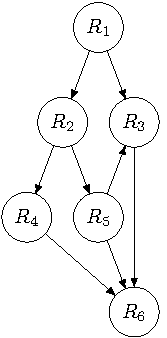
\includegraphics[width=2in]{bn_simple_crop.pdf}
					\caption{Simple Bayesian network.} 
					\label{fig:Eg BN}
				\end{center}
			\end{figure}

			Such networks encodes the conditional independence properties of the distribution~\citep{nilsson1998artificial}.
			
			\begin{prop} \textbf{(Conditional independence for Bayesian networks)}\\ 
				In a Bayesian network, each node of the graph are conditionally independent of any subset of the nodes that are not descendants of itself given its parent.
				
				\begin{equation}
				  P(\{R_{i}\}_{i \in \llbracket1,N \rrbracket}) = \prod_{i=1}^{N} P(R_{i} | R_{\rho(i)})
				  \label{eq:BN CI}
				\end{equation}
				
				where $R_{\rho(i)}$ are the parents of the node $R_{i}$. 
				\label{pty:CI for BNs}
			\end{prop}
			
			Thus in such a network, a node with no parents is not conditioned on any other random variable considered and defines a prior probability.\\

			Using Property~\ref{pty:CI for BNs} allows to simplify the computation of the joint probability distribution. For example for the network defined in Figure~\ref{fig:Eg BN}, one can obtain $P(R_{1},R_{2},R_{3},R_{4},R_{5},R_{6})$ using the chain rule and theory on conditional independent,
			
			\begin{equation*}
			  \begin{split}
			    P(R_{1},R_{2},R_{3},R_{4},R_{5},R_{6})
						&= P(R_{6} | R_{3},R_{4},R_{5}) P(R_{1},R_{2},R_{3},R_{4},R_{5}) \\
						&= P(R_{6} | R_{3},R_{4},R_{5}) P(R_{3} | R_{1},R_{5}) P(R_{4}| R_{2}) P(R_{5}| R_{2}) P(R_{1},R_{2})\\
						&= P(R_{6} | R_{3},R_{4},R_{5}) P(R_{3} | R_{1},R_{5}) P(R_{4}| R_{2}) P(R_{5}| R_{2}) P(R_{2}|R_{1}) P(R_{1}).\\
			  \end{split}
			  \label{eq:Eg BN CI}
			\end{equation*}
      
%       are directed acyclic graphs whose nodes represent random variables in the Bayesian sense. Those nodes can be observable quantities, latent variables, unknown parameters or hypothesis. Edges of the graph represent conditional dependencies between the variables.  nodes that are not connected represent variables that are conditionally independent of each other. Each node is associated with a probability function that takes, as input, a particular set of values for the node's parent variables, and gives (as output) the probability (or probability distribution, if applicable) of the variable represented by the node. For example, if m parent nodes represent m Boolean variables then the probability function could be represented by a table of 2^m entries, one entry for each of the 2^m possible combinations of its parents being true or false


    \subsection{Inference:}
      \label{subsec:PGMs/BN/Inference}
      
			A Bayesian network encodes the full joint distribution of the studied random variables. This knowledge can be used to perform several interesting inference taks among which are:\\
     % see http://www.ee.columbia.edu/~vittorio/lecture12.pdf
				
     \begin{itemize}
        \item Belief updating: Given some evidences ---\ie: values for some nodes of the network $\{R_{j}\}_{j \in J}$ where $J$ is a subset of the graph--- on is interested in the probability associated with an unobserved variable,
        
        \begin{equation}
					R_{i}^{\ast} = P(R_{i}|\{R_{j}\}_{j \in J}).
					\label{eq:BN inference BEL}
				\end{equation}
				
				Selecting the $R_{i}$ maximising this probability is the prediction for this node. The advantages of belief updating over other prediction method as it can provide a probabilistic prediction even when given incomplete observations ---\ie a set $\{R_{j}\}_{j \in J}$ such that $J \cup \{i\} \neq \bfR$. Belief updating can be extended to the prediction of a set of unobserved variables.\\
				
				\item Optimal decision: A probabilistic graphical model can be used to express actions taken by an agent to modify the state of an uncertain world. In this case given some evidences $\{R_{j}\}_{j \in J}$ where $J$ is a subset of the graph $\mcalG$ one is interested in finding the set of action $\{A_{i}\}_{i \in \mcalA}$ where $\mcalA$ is the set of all possible actions. To do so one also needs a reward function $O_{i}(A_{i})$ expressing the outcome of the action $A_{i}$,  maximizing the probability of the outcome $\O$,

				\begin{equation}
					\{A_{i}^{\ast}\}_{i \in \mcalA} =\argmax_{\mcalA} P(\{O_{i}(A_{i})\}_{i \in \mcalA} | \{A_{i}\}_{i \in \mcalA}, \{R_{j}\}_{j \in J}).
					\label{eq:BN inference optimal decision}
				\end{equation}
				
				This type of inference is useful in Reinforcement learning framework where one is interested in learning the optimal set of actions to complete a task.\\
				
				\item Sensitivity analysis: Given some evidences ---\ie: values for some nodes of the network $\{R_{j}\}_{j \in J}$ where $J$ is a subset of the graph--- used for belief updating, one can be interested in assessing which among those random variables as the most influence on the prediction quality. This means find,
				
				\begin{equation}
					\Delta_{k}^{\ast}= \argmax_{k \in J} \Delta_{k}
					\label{eq:BN Sensitivity analysis 1}
				\end{equation}
				
				where $\Delta_{k}$ defines the difference between the probabilities given the full set of evidences and given the set minus the $k$-th evidence,
				
        \begin{equation}
					\Delta_{k} = P(R_{i}|\{R_{j}\}_{j \in J}) - P(R_{i}|\{R_{j}\}_{j \in J\backslash \{k\}}).
					\label{eq:BN Sensitivity analysis 2}
				\end{equation}      
      
				This type of inference can be useful in the case where the evidences are expensive to collect, or when prediction has to be provided within a certain time. Then the sensitivity analysis allows to focus the effort into collecting/incorporating the most important piece of information.       
      \end{itemize}

    \subsection{Learning:}
      \label{subsec:PGMs/BN/Learning}
     
      In most applications, the full characterization of the BN is not provided but has to be learned from a set of observations $\bfX = \{\bfx_{n}\}_{n\in \llbracket 1,N \rrbracket}$. One can split the learning problem into two main categories:\\
      
      \begin{itemize}
				\item Learning the local probability distributions: In this case the structure of the graph $\mcalG$ is known and fixed before hand. It can be provided by an expert (e.g. IBM trouble shooting system~\citep{rish2002efficient}) or be imposed by some construction rules (e.g. Boltzmann Machine~\citep{ackley1985learning}, Restricted Boltzmann Machine~\citep{smolensky1986information} ...). The task at hand is then to learn the parameters $\Theta$ governing the local probability distributions of the network.\\
				
        \item Learning the architecture and local probability distributions: In this case the architecture of the network $\mcalG$ has to be learned along side with the local probability distributions' parameters $\Theta$. This problem is not developed in the rest of this paper, but one could refer to~\citep{margaritis2003learning} for an introduction to the existing methods.\\
      \end{itemize}
      
      Leaving aside the case where the network architecture has to be learned, the problem of learning the parameter of a Bayesian network can again be split into two main categories. 
      
      \subsubsection{Complete data:}

				In this case each training example of the set $\bfX$ contains the value of the full set of random variable $\bfR$ of the graph. In such a case one can use methods such as the Maximum Likelihood estimates where the parameters of the network are selected to maximize the log-likelihood of the data given the model,
				
      \begin{equation}
        \Theta_{ML} = \argmax_{\Theta} \log P(\bfX | \Theta).
        \label{eq:BN ML}
      \end{equation}
      
      Another common estimator used is the Maximum A Posteriori (MAP) estimate where one maximize the posterior distribution of the network's parameters given the data,
      
      \begin{equation}
        \Theta_{MAP} = \argmax_{\Theta} \log P(\Theta | \bfX) = \argmax_{\Theta} \log (P(\bfX | \Theta)P(\Theta)). 
        \label{eq:BN MAP}
      \end{equation}    
      
      While the MAP estimate describe the full distribution of the parameters $\Theta$ over the observations, ML provides only a point-wise estimate. However ML is often preferred as MA can be intractable.
      
      \subsubsection{Incomplete data:}

				In this case each training example of the set $\bfX$  only contains the value of some random variable $\{R_{i}\}$ of the graph. In such a case one has to use a two steps iterative algorithm named the Expectation-Maximisation (EM) algorithm. The first step (Expectation) aims at estimating the values of the unobserved random variables given the current estimate of the parameters $\Theta$, while the Maximisation step aims at providing a ML estimate of $\Theta$ once all the variable are known or estimated. This procedure is described in more details in Section~\ref{sec:SCHMT/Learning}.
				
  \section{Markov Models:}
    \label{sec:PGMs/MM}
    Markov models are a subclass of graphical models useful when it comes to describing a system whose observations are randomly changing over an event. The key assumption in those models is that the upcoming observation only depends on a finite number of previous ones.
    
    \begin{equation}
      \forall t \in \dsN \;\;\; P(\text{obs}_{t+1} \; | \; \{\text{obs}_{k}\}_{k \in \dsN}) \;\; = \;\; P(\text{obs}_{t+1} \; | \; \{\text{obs}_{k}\}_{k \in \llbracket t-l, t \rrbracket})
      \label{eq:MM assumtion v1}
    \end{equation}
    
    where $l \in \dsN$ characterized the number of past steps used to condition the next observation. Most of the time, for sake of computational tractability as well as because this constraint seems to be sufficient, the future observation is assumed to be only dependent on the present one.  

    \begin{equation}
      \forall t \in \dsN \;\;\; P(\text{obs}_{t+1} \; | \; \{\text{obs}_{k}\}_{k \in \dsN}) \;\; = \;\; P(\text{obs}_{t+1} \; | \text{obs}_{t})
      \label{eq:MM assumtion v2}
    \end{equation}
    
    Maybe the most famous class of Markov model is the Markov chain. It has applications in finance (Brownian motion~\citep{duncan2000stochastic}), in Internet page ranking (Google page rank~\citep{haveliwala2003second}) or as a sampling procedure (Markov Chain Monte-Carlo (MCMC)~\citep{gilks2005markov}). Those models are not covered in this document but~\citep{kemeny1960finite} provides a good entry point to the field for reader with further interests for Markov chains.\\
    
    Another flavour of Markov models are the Hidden Markov Models (HMMs). The remainder of this section is dedicated to providing a general introduction to those models. While Subsection~\ref{subsec:PGMs/MM/Architecture} formalizes the HMM modelling, Subsection~\ref{subsec:PGMs/MM/Inference} and~\ref{subsec:PGMs/MM/Learning} respectively describes the inference mechanism and the learning method for HMMs.    
    
    \subsection{Architecture:}
      \label{subsec:PGMs/MM/Architecture}
      
      An HMM is a stochastic finite automaton, where each hidden state generates ---\ie emits--- an observation. Let $O_{t}$ be the observation at step $t$ and $H_{t}$ denotes the hidden state at this step. Let also $K_{t}$ be the number of possible states at step $t$ such that $H_{t} \in \llbracket 1, K_{t} \rrbracket$. The observations in an HMMs can be discrete, continuous or mixed.\\
      
      The model's parameters are:\\ 
      
      \begin{itemize}
        \item The initial state distribution $\pi(i) = P(H_{0} = i)$ where $\pi$ is a multinomial distribution.\\
        \item The transition model at step $t$, $\epsilon_{t}^{(ij)} = P(H_{t+1} = j | H_{t} = i)$ where $\epsilon_{t}$ is a stochastic matrix.\\
        \item The emission model $P(O_{t}|H_{t})$. Usually the emission model is defined by a parametric distribution governed by $\theta_{k,t}$. In the case of discrete observations,  it is defined by a multinomial distributions such that,
					\begin{equation*}
						\forall t \geq 0 \;\;\; \forall (l,k) \in |O_{t}| \times \llbracket 1, K_{t} \rrbracket \;\;\;
						P(O_{t}= l| H_{t}=k) = P_{\theta_{k,t}}(l).
					\end{equation*}
					where $|O_{t}|$ is the set of value for $O_{t}$. In the continuous case, the observation model is a continuous parametric distribution such that,
					\begin{equation*}
						\forall t \geq 0 \;\;\; \forall (l,k) \in \dsR^{d_{t}} \times \llbracket 1, K_{t} \rrbracket \;\;\;
						P(O_{t}= l| H_{t}=k) = P_{\theta_{k,t}}(l).
					\end{equation*}
					where $d_{t}$ is the dimension of $O_{t}$.\\
					
      \end{itemize}

      A common simplification to those model is to assume stationarity. This means stating that the transition matrices and observation models are shared across steps. 
      
    \subsection{Inference:}
      \label{subsec:PGMs/MM/Inference}
      
      HMMs are probabilistic graphical models encoding the joint distribution of the system. Hence they can be used to perform similar inference tasks as those described in Sub-section~\ref{subsec:PGMs/BN/Inference} for Bayesian networks, with the difference that for HMMs, the values of the hidden states have to be inferred prior to solving any specific request.\\
      
      Infer the value of the hidden states can be done using a MAP estimate adapted to HMMs. The initial MAP  algorithm is due to~\citet{viterbi1967error} and was originally designed to analyse Markov processes observed in memoryless noise. \citet{forney1973viterbi} expressed this algorithm as being equivalent to finding the shortest path in a graph with weighted edges.\\
      
      \begin{note}
        This procedure is described at length in the special case of hidden Markov trees in Section~\ref{sec:SCHMT/Clf} but this section aims at providing an informal explanations on the methodology.\\
      \end{note}
      
      The observation behind Viterbi's MAP algorithm for HMMs is that for any state at step $t$, there is only on most likely path to this state. Therefore, one can simplify the computation by replacing several paths converging to a given state at step $t$ by simply the most likely one. Applying this method at each step of the model reduces the computation complexity from $\mcalO(K^{t})$ to $\mcalO(T.K^{2})$.\\
      
    \subsection{Learning:}
      \label{subsec:PGMs/MM/Learning}
      
      Learning the parameters of an HMM from data is somehow similar to learning the parameters of a Bayesian network in the case of incomplete data, as only parts of the nodes of an HMM are observed. Hence the parameters of an HMM model can be learned using an offline maximum likelihood (ML) estimation method known as the EM --- or Baum-Welch--- algorithm.\\
      
      Let $\{O_{[1:T]}^{n}\}_{n \in \llbracket 1,N \rrbracket}$ be a set of observed nodes of an HMMs used as training set. The learning procedure would be straight forward if one had access to the sequences of hidden state $H_{[0:T]}^{n}$ for all $n \in \llbracket 1,N \rrbracket$. In this case, the ML estimate of the transition matrix could be computed by normalizing the matrix of co-occurrences,
      
      \begin{equation}
        \epsilon_{t,ML}^{(ij)} = \frac{C_{t}(i,j)}{\sum_{k=1}^{K}C_{t}(i,k)}
        \label{eq:EM intuit transition}
      \end{equation}
      
      where 
      \begin{equation}
        C_{t}(i,j) = \sum_{n=1}^{N} \ds1(H_{t+1}=j, H_{t}=i)
        \label{eq:EM intuit transition count}
      \end{equation}
      
      and $\ds1(\text{event})$ is the binary indicator of occurrence of a event. The initial distribution and the observation model could be estimated in a similar fashion.\\
      
      However since $H_{[0:T]}^{n}$ is hidden, one have to estimate the hidden states prior to performing the ML update. The rough idea of the EM-algorithm is to estimate the hidden states given the observations using a the Maximum A Posteriori approached described in the previous section with the current set of parameters. This is the Expectation (E) step. Those estimated sequences of hidden state are then used to update the parameters' estimate. This is the Maximisation (M) step.\\
      
      One can prove~\citep{baum1970maximization}~\citep{dempster1977maximum} the convergence of this procedure toward a ---local--- maximum of the the likelihood.
      
      
%%%%%%%%%%%%%%%%%%%%%%%%%%%%%%%%%%%%%%%%%%%%%%%%%%%%%%%%%%%%%%%%%%%%%%%%%%%%%%%%%%%%%%%%%%%%%%%%%%%%%%%%%%%%%%%%%%%%%%%%%%%%%%%%%%%%%%%%%%%%%%%%%%%%%%%%%%%%%%%%%%%%%%%%%%%%%%%%%%%%%%%%%%%%%%%%%%%%%%%%%%%%%%%%%%%%%%%%%%%%%
%%%%%%%%%%%%%%%%%%%%%%%%%%%%%%%%%%%%%%%%%%%%%%%%%%%%%%%%%%%%%%%%%%%%%%%%%%%%%%%%%%%%%%%%%%%%%%%%%%%%%%%%%%%%%%%%%%%%%%%%%%%%%%%%%%%%%%%%%%%%%%%%%%%%%%%%%%%%%%%%%%%%%%%%%%%%%%%%%%%%%%%%%%%%%%%%%%%%%%%%%%%%%%%%%%%%%%%%%%%%%
%%%%%%%%%%%%%%%%%%%%%%%%%%%%%%%%%%%%%%%%%%%%%%%%%%%%%%%%%%%%%%%%%%%%%%%%%%%%%%%%%%%%%%%%%%%%%%%%%%%%%%%%%%%%%%%%%%%%%%%%%%%%%%%%%%%%%%%%%%%%%%%%%%%%%%%%%%%%%%%%%%%%%%%%%%%%%%%%%%%%%%%%%%%%%%%%%%%%%%%%%%%%%%%%%%%%%%%%%%%%%
\chapter{Scattering convolutional hidden Markov trees:}
  \label{chap:SCHMT}
  Section~\ref{sec:ST/Applications to clf} introduced the use of scattering networks combined with a support vector machine classifier to achieve competitive classification performance on some problems. However this method provides a boolean label for each class. Some methods to express the output of an SVM as a probability exists~\citep{platt1999probabilistic} but they are just a rescaling of the output and not a true probabilistic approach. If one is interested in a true probabilistic model to describe the scattering coefficients, it is quite natural to try expressing them as a probabilistic graphical model. Indeed if one ignores the propagation step from the scattering transform (see Section~\ref{sec:ST/SCN}) the scattering network defines the tree structure displayed in Figure~\ref{fig:ST tree}. \\

	\begin{figure}[h]
			\begin{center}
				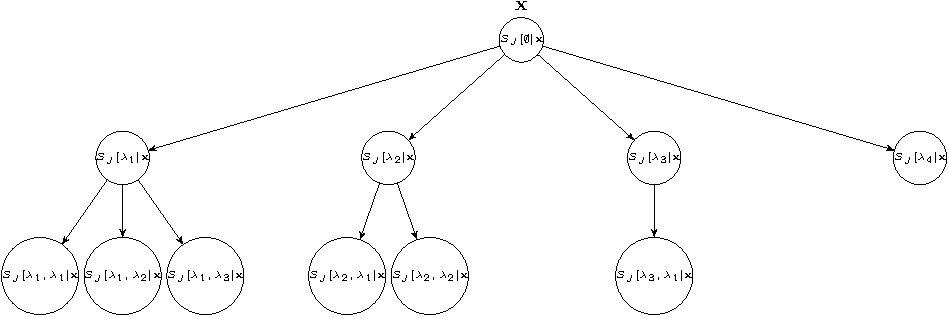
\includegraphics[width=5in]{scat_tree_crop.pdf}
				\caption{Scattering transform tree.}
				\label{fig:ST tree}
			\end{center}
	\end{figure}
  
  To simplify notations in the remainder of this section, let $\mcalT$ denotes the tree structure defined by a scattering convolutional network $ST_{(\psi, J, M, L)}(.)$ restricted to frequency decreasing path of length shorter than $M$, considering $J$ scales and $L$ orientations. This tree $\mcalT$ depicted in Figure~\ref{fig:ST tree}.  Let $I$ denotes the total number of nodes ---\ie scattering coefficients--- and let $S_{i}$ for $i \in \llbracket0, I-1 \rrbracket$ denotes one of the node of $\mcalT$ for a given path $p_{i} = [\lambda_{0} ... \lambda_{u}]$ ($u\in \dsN$). Note that $S_{i}$ represents a node and does not depends on the signal $\bfx$. For a given signal $\bfx$, the realization of the node $i$ for signal $\bfx$ is denoted by $S_{i}= s_{i} = S[p_{i}]\bfx$. Note also that in the remainder of the paper the shorter notation $i \in \mcalT$ will be used to denote the path $p_{i}$ to the node $i$. Let also use the convention $S_{0} = S[\emptyset](.)$. Finally let $\rho_{i}$ and $\mcalC(i)$ denote respectively the parent of a node $i$ and the set of children of the node $i$. A node $S_{i}$ can have no children, in such a case this node is a leaf of the tree.\\
  
  The remainder of this section is organized as follows: Section~\ref{sec:SCHMT/Rel work} introduces related work and provides a description of our proposed SCHMT model. Section~\ref{sec:SCHMT/Hypos} details the hypothesis needed to develop this model as well as provides some intuitions on their validity. Finally Section~\ref{sec:SCHMT/Learning} and~\ref{sec:SCHMT/Clf} respectively describe the proposed algorithm for learning the parameters of an SCHMT and the classification method.

  
  \section{SCHMT model and related works:}
    \label{sec:SCHMT/Rel work}
      
    The idea behind the SCHMT model is to assume that the more detailed representation of the signal is somehow correlated to the less detailed one from which it is generated. More formally this means that for a signal $\bfx$, $s_{i}$ is somehow correlated to $s_{\rho(i)}$. This assumption yields a modelling of the scattering network by a Markov tree and assumes,
    
    \begin{equation}
      P(S_{i} |\mcalT) = P(S_{i} | S_{\rho(i)}).
      \label{eq:SMT - false hypo}
    \end{equation}\\

    Those independence properties are encoded in the graph displayed in Figure~\ref{fig:ST tree}. M
odels trying to describe directly the correlation across coefficients at different scales have been studied for traditional wavelet transforms~\citep{lee1996new} but are in conflict with the compression property of the wavelet ---\ie the fact that most wavelet representations are sparse~\citep{crouse1998wavelet}. Thus it seems that a simple one-step Markovian assumption across scale is not satisfying to describe the complex relationship between wavelet or scattering coefficients.\\
    
    A common approach when a direct Markovian model does not hold is to introduce hidden states and assume the Markovian property across those unobserved states. The observed nodes being then only dependent on their respective state. This architecture has been adopted to create the SCHMT. This model is represented by Figure~\ref{fig:SCHMT 1} and it induces the following independence properties,
    
    \begin{equation}
      P(H_{i} |\mcalT) = P(H_{i} | H_{\rho(i)}),
      \label{eq:SCHMT - hypo 1}
    \end{equation}    
    \begin{equation}
      P(S_{i} |\mcalT) = P(S_{i} | H_{i}).
      \label{eq:SCHMT - hypo 2}
    \end{equation} \\
    
		\begin{figure}[h]
				\begin{center}
					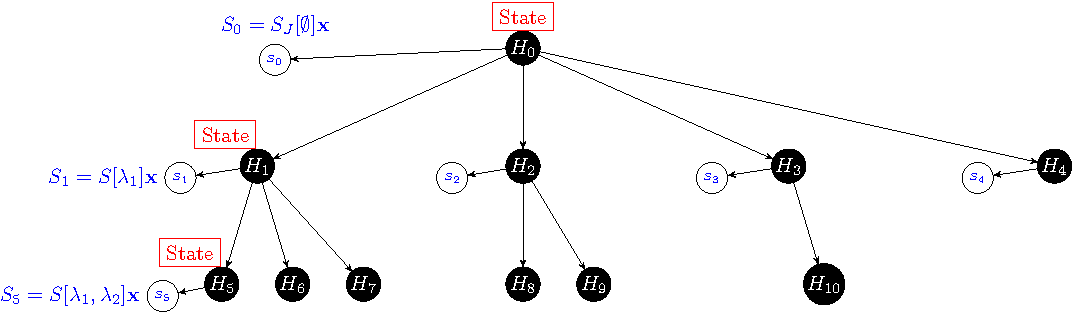
\includegraphics[width=5in]{scat_HMT_crop.pdf}
					\caption{Scattering convolutional hidden Markov tree.}
					\label{fig:SCHMT 1}
				\end{center}
		\end{figure}
		
		As the scattering transform is closely related to wavelet transform it is not surprising to find similar ideas exploited for wavelet trees. \citet{crouse1998wavelet} have developed a model where a Hidden Markov Tree Model is used to model the wavelet coefficients of a standard wavelet trees. Later \citet{kingsbury2001complex} has  adapted Crouse's model to his Dual Wavelet Complex Trees. The resulting hidden Markov tree models provides better classification performance than Crouse's Wavelet Hidden Markov Tree (WHMT) as the wavelet used generates a ``better'' representation of the signal in the sense defined in Section~\ref{sec:Intro/Signal rep/Intuition}. Indeed this version can leverage the quasi-translation invariance property of the complex wavelets. This improvement in performance due to the quasi-invariance property provides a good motivation for using a hidden Markov tree model on the scattering transform as they have even ``better'' representational properties (see Section~\ref{sec:ST/Pties}). The parameters of the original WHMT are trained using a version of the Expectation-Maximization adapted to binary hidden Markov trees. However since this learning method suffers from underflowing issues~\citep{devijver1985baum}, \citet{durand2004computational} proposed a smoothed version of the training algorithm preventing this from happening.\\
     
	  We propose an adaptation of those models to create a scattering convolutional hidden Markov tree composed of a set of visible nodes $\{\bfS_{i}\}_{i \in \mcalT}$ and a set of hidden node $\{\bfH_{i}\}_{i \in \mcalT}$. Both sets are organized in a tree structure with the following characteristics,\\
	  
    \begin{itemize}
      \item For any index $i$ of the tree, $S_{i} \in \dsR$ and $H_{i} \in \llbracket 1,K \rrbracket$ where $K$ is the number of possible hidden states.\\
      
      \item The initial hidden state is drawn from a discrete non uniform initial distribution $\pi_{0}$ such that:
	  	  \begin{equation}
					\forall k \in \llbracket 1,K \rrbracket \;\;\; \pi_{0}(k) = P(H_{0}=k).
					\label{eq:SCHMT - initial distribution}
				\end{equation}\\
				
      \item For any index $i$ of the tree, the emission distribution describes the probability of the visible node $S_{i}$ conditional to the hidden state $H_{i}$,
				\begin{equation}
				  \forall i \in \mcalT \;\; \forall k \in \llbracket1,K\rrbracket \;\; \text{and} \;\; \forall s \in \dsR
					\;\;\;\;\;\; P(S_{i}=s_{i}|H_{i}=k) = P_{\theta_{k,i}}(s),
					\label{eq:SCHMT - Emission distr}
				\end{equation}
			where $P_{\theta_{k,i}}$ belongs to a parametric distribution family and where $\theta_{k,i}$ is the vector of emission parameters for the state $k$ and the node $i$. In the remainder of the paper the emission distribution is Gaussian so that,  
      	\begin{equation}
				  \forall i \in \mcalT \;\; \forall k \in \llbracket1,K\rrbracket \;\; \text{and} \;\; \forall s \in \dsR
					\;\;\;\;\;\; P(S_{i}=s | H_{i}=k) = \mcalN(\mu_{k,i},\sigma_{k,i}),
				  \label{eq:SCHMT - Mixt of Gaussian}
				\end{equation}
				where $\theta_{k,i}=(\mu_{k,i},\sigma_{k,i})$ with $\mu_{k,i}$ and $\sigma_{k,i}$ being respectively the mean and the variance of the Gaussian for the $k$-th value of the mixture and the node $i$.\\
				
			\item For any index $i$ of the tree, the probability for the hidden node $H_{i}$ to be in a state $k$ given the father's state $g$ is characterized by a transition probability,
				\begin{equation}
					\forall i \in \mcalT \backslash \{ 0 \} \;\;\; \forall g,k \in \llbracket1,K\rrbracket^{2}
					\;\;\;\;\;\; \epsilon_{i}^{(gk)} = P(H_{i}= k | H_{\rho(i)}=g), 
					\label{eq:SCHMT - Transition matrix}
				\end{equation}
				where $\epsilon_{i}$ defines a transition probability matrix such that,
				\begin{equation}
				  \forall i \in \mcalT \backslash\{0\} \;\;\;  \forall k \in \llbracket1,K\rrbracket
					\;\;\;\;\;\;  P(H_{i}=k) = \sum_{g=1}^{K} \epsilon_{i}^{(gk)} P(H_{\rho(i)}=g). %TODO: Check if it is conditional or not.
				  \label{eq:SCHMT - State proba 1}
				\end{equation}
				Note that using the chain rule of probability one can express $P(H_{i})$ from the root node's initial distribution.\\
				%TODO: find this formula in Durand article
		\end{itemize}
		
		Thus for a given scattering architecture ---\ie fixed $M$, $J$ and $L$--- the SCHMT model is fully parametrized by,
		
		\begin{equation}
			\Theta = \big(\pi_{0}, \{ \epsilon_{i}, \{ \theta_{k,i} \}_{k\in\llbracket1,K\rrbracket} \}_{i\in\mcalT}\big).
			\label{eq:SCHMT - parameters}
		\end{equation}
		
    Our SCHMT model differs from the previous works by the properties of its tree structure. Previous works are based on regular binary trees where all the leaves have the same depth while the scattering tree is both irregular and non-binary. Indeed as seen in Section~\ref{sec:ST/SCN} each node has a variable number of children, which yields an architecture where the number of descendants is not constant and where leaves can be found at any depth of the tree. Another difference between SCHMT and the previous works is the non-homogeneity of the transition matrix. Indeed by the nature of the scattering transform one can expect a non homogeneous transmission of the information across the orders and especially across the orientations. Hence non-homogeneous transition matrices across nodes from a same father and across images themselves are allowed. Section~\ref{sec:SCHMT/Learning} describes an adaptation of \citet{durand2004computational} learning algorithm to an irregular, non-homogeneous and non-binary trees.\\
    
    Even though the theoretical framework of SCHMT holds for any $K \in \dsN^{\ast}$, in all the applications of the SCHMT we set $K=2$. This means that the scattering coefficients are described by a mixture of two Gaussians and can be in either $(L)$ Large or $(S)$ Small. This model yields a sparser representation of the scattering coefficient as the number of hidden states is highly constrained.
    
    
  \section{Hypothesis:}
    \label{sec:SCHMT/Hypos}
    
    Expressing the dependencies between the scattering coefficients as a Hidden Markov Tree implies two modelling assumptions. The first one reflects the fact that the scattering coefficients can effectively be expressed by two hidden states,\\
    
    \begin{assumption}\textbf{$K$ populations:}\\
			A signal's scattering coefficients can be described by $K$ clusters. The smooth regions are represented by small scattering coefficients, while edges, ridges, and other singularities are represented by large coefficients.\\
			\label{assum:2pop}
    \end{assumption}
    
    As this assumption is common for standard or complex wavelets~\citep{kingsbury2001complex} and because a scattering coefficient of order $m$ can simply be seen as the modulus of the wavelet transform of a ``new'' signal ---\ie the scattering coefficient of order $m-1$, the two-populations assumption for scattering network is reasonable.\\
    
    This intuition can be confirmed by Figure~\ref{fig:2pop - 1} and~\ref{fig:2pop - 2} displaying the scattering coefficients at a given node obtained for several signals. Figure~\ref{fig:2pop - 1} shows the scattering coefficients of a noisy binary square. Note that for sake of clarity a ``small'' network has been used. This does not affect the observations that can be made and one can notice that the largest values of the scattering coefficient are obtained on highly informative pixels (edges in this case) while the less informative pixels are represented by scattering coefficients near $0$. Similar observations can be made for more complex signals ---such as the one displays in Figure~\ref{fig:2pop - 2}.\\
 
		\begin{figure}[h]
			\centering
			\begin{subfigure}[t]{0.48\textwidth}
				\centering
				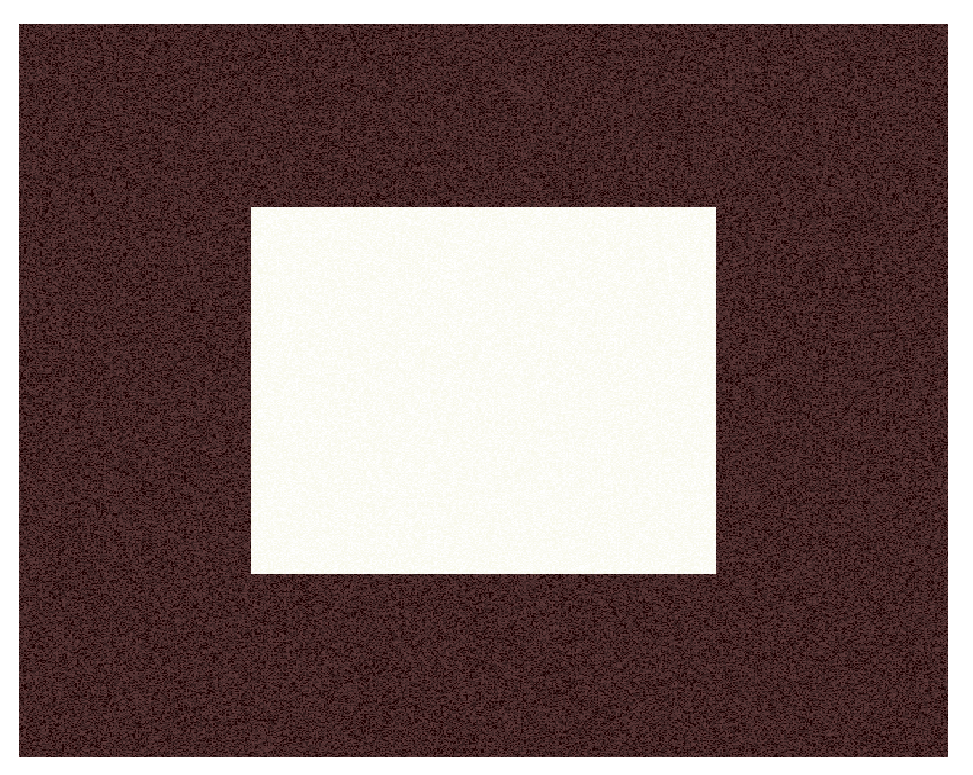
\includegraphics[height=2.3in]{2pop_square_original.eps}
				\caption{Original}
			\end{subfigure}%
			~
			\begin{subfigure}[t]{0.48\textwidth}
				\centering
				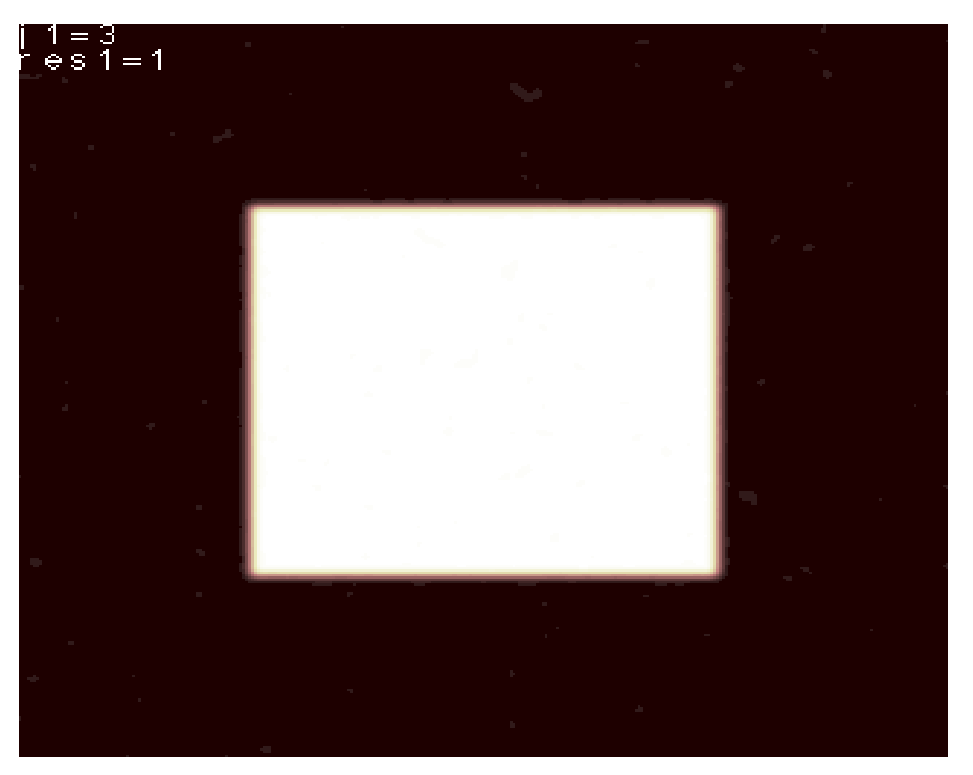
\includegraphics[height=2.3in]{2pop_square_layer0.eps}
				\caption{Layer 0}
			\end{subfigure}%
			\\ 
			~
			\begin{subfigure}[t]{0.48\textwidth}
				\centering
				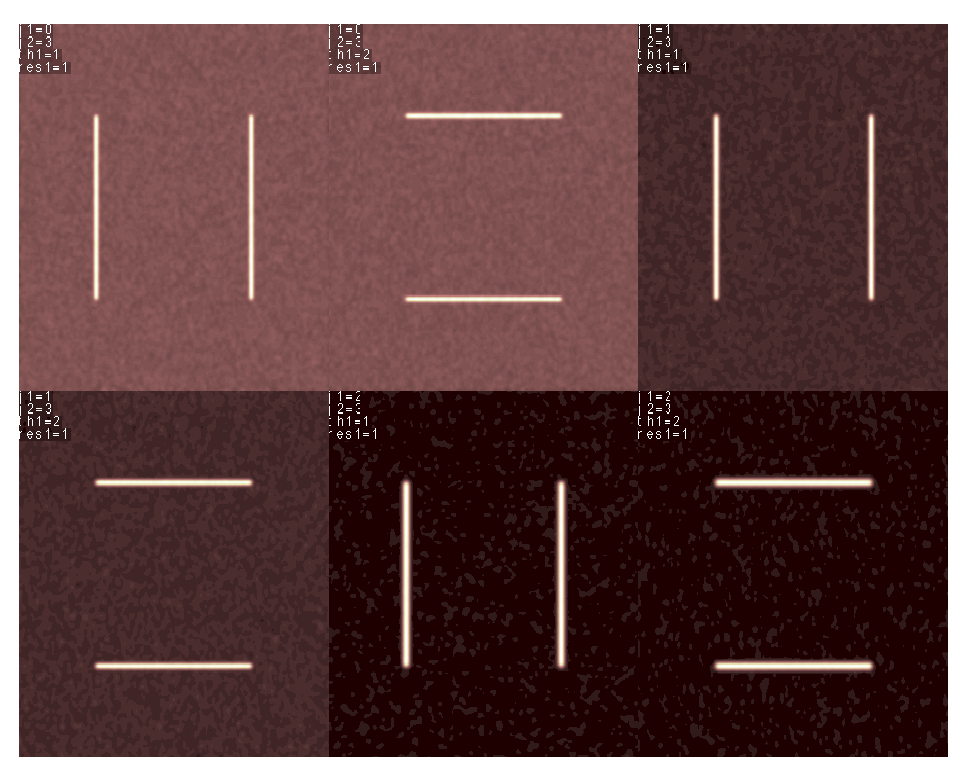
\includegraphics[height=2.3in]{2pop_square_layer1.eps}
				\caption{Layer 1}
			\end{subfigure}
			~ 
			\begin{subfigure}[t]{0.48\textwidth}
				\centering
				\includegraphics[height=2.3in]{2pop_square_layer2.eps}
				\caption{Layer 2}
			\end{subfigure}
					
			\caption[$K$ populations - Experiment 1.]{\centering $K$ populations - Experiment 1: The signal is a binary square (0: background, 1: square) with noise. The scattering network has $M=2$ layers, $J=3$ scales and $L=2$ orientations.}
			\label{fig:2pop - 1}
		\end{figure}
 
 
		\begin{figure}[h]
			\centering
			\begin{subfigure}[t]{0.48\textwidth}
				\centering
				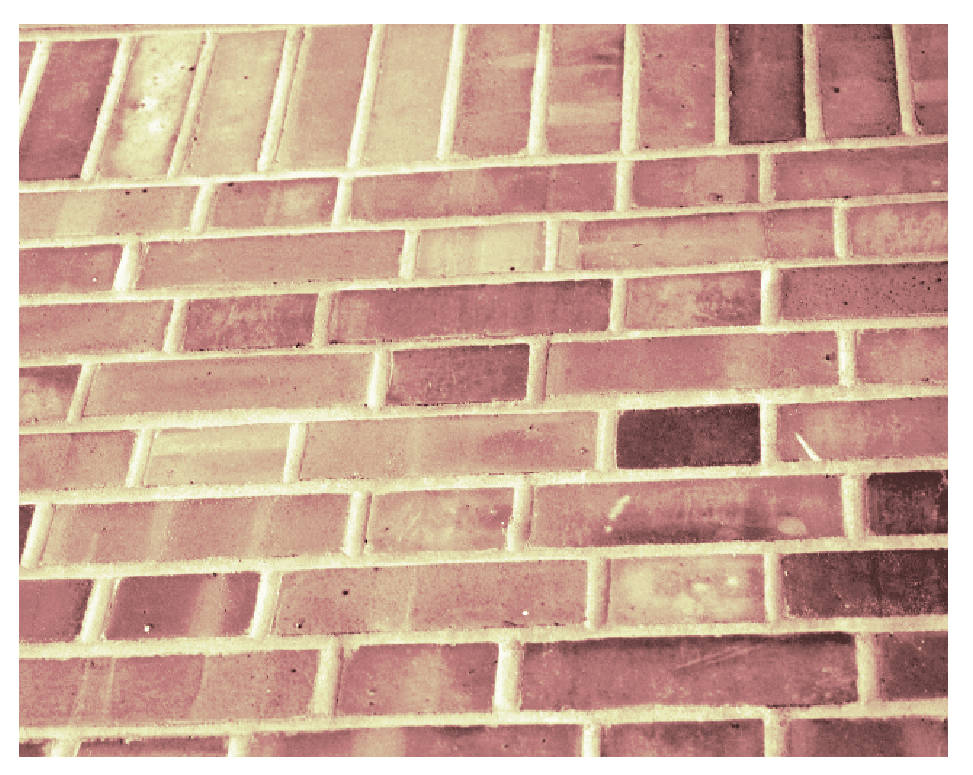
\includegraphics[height=2.3in]{2pop_uiuc_original.eps}
				\caption{Original}
			\end{subfigure}%
			~
			\begin{subfigure}[t]{0.48\textwidth}
				\centering
				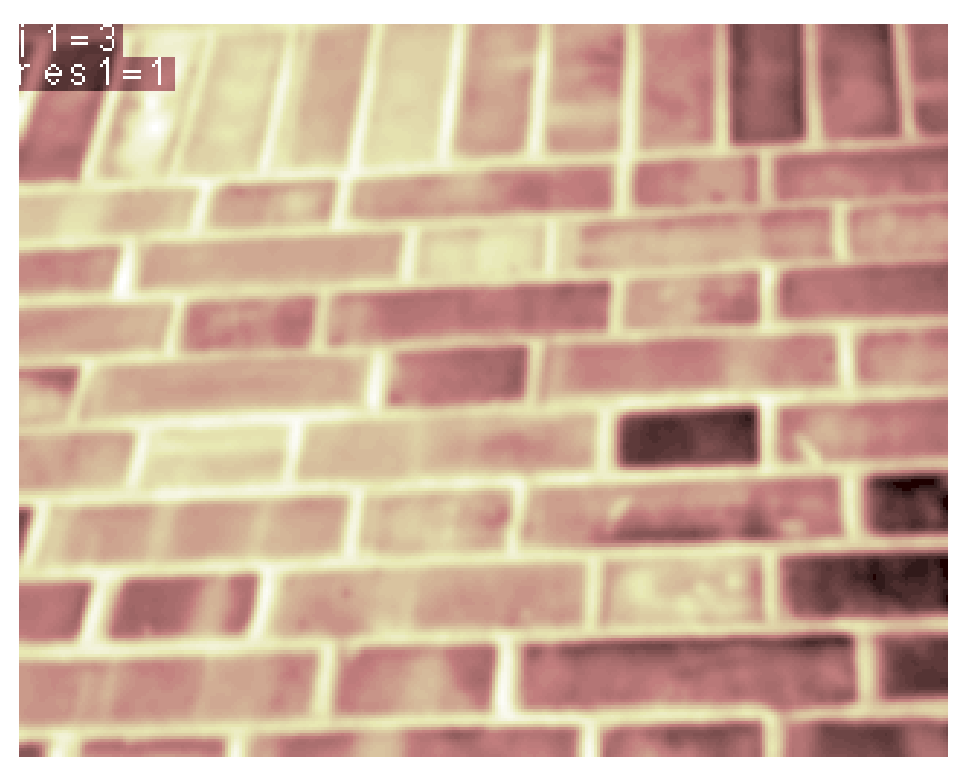
\includegraphics[height=2.3in]{2pop_uiuc_layer0.eps}
				\caption{Layer 0}
			\end{subfigure}%
			\\
			~
			\begin{subfigure}[t]{0.48\textwidth}
				\centering
				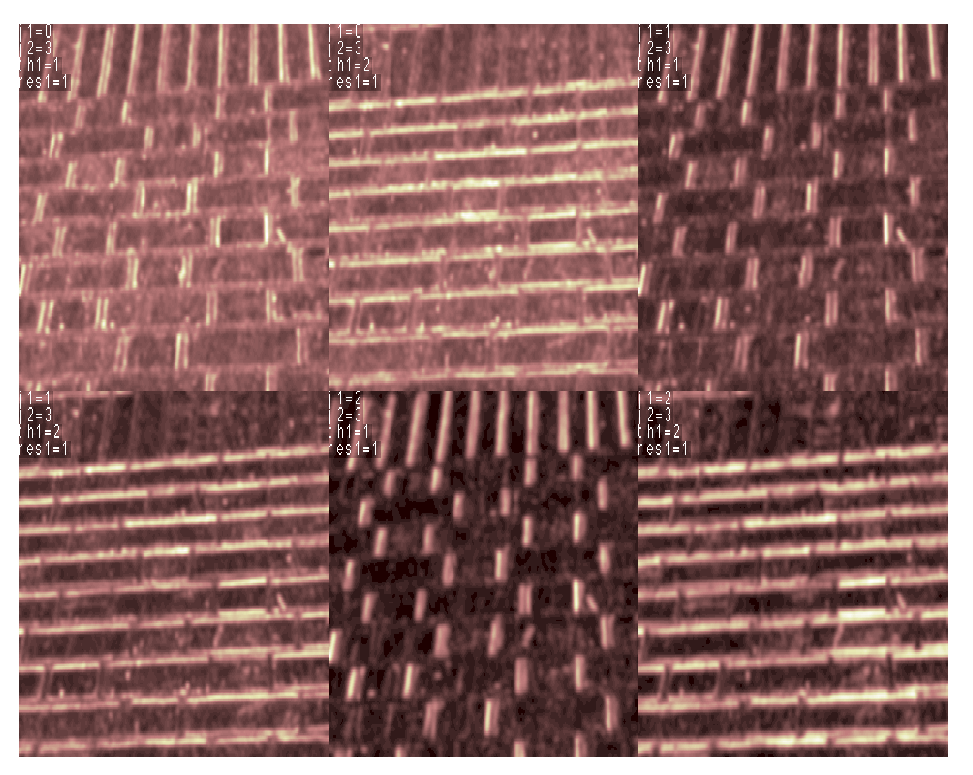
\includegraphics[height=2.3in]{2pop_uiuc_layer1.eps}
				\caption{Layer 1}
			\end{subfigure}
			~ 
			\begin{subfigure}[t]{0.48\textwidth}
				\centering
				\includegraphics[height=2.3in]{2pop_uiuc_layer2.eps}
				\caption{Layer 2}
			\end{subfigure}
			\caption[$K$ populations - Experiment 2.]{\centering $K$ populations - Experiment 2: The signal is a realisation of the class ''brick wall'' of the \textit{CUReT} texture dataset. The scattering network has $M=2$ layers, $J=3$ scales and $L=2$ orientations.}
			\label{fig:2pop - 2}
		\end{figure}

		A statistical interpretation of the $K$ populations assumption implies that scattering coefficients have non-Gaussian marginal statistics, that is, their marginal probability density functions have a large peak at zero due to the many small coefficients and heavy tails a few large coefficients are observed. Finally since many real-world signals (photograph-like images, for example) consist mostly of smooth regions separated by a few singularities, the $K$ populations assumption tells us that the scattering coefficients are a sparse representation for these signals (this notion of sparsity can be made mathematically precise; see for example~\citep{donoho1993unconditional} or~\citep{devore1992image}). Most of the scattering coefficient magnitudes are small, while a few of them encoding the singularities and the informative content are large.\\
		
		The second assumptions expresses the smoothness of the states across the scattering transform.\\
		
		\begin{assumption}\textbf{Persistence:}\\
		  Along a scattering path, high and low scattering coefficient values cascade across the scattering orders.\\
		  \label{assum:Persistence}
		\end{assumption}

		This assumption codifies how the hidden states are structured. Smooth regions/singularities are assumed to be represented by low/high values at every layer. Persistence leads to scattering coefficient values that are statistically dependent along the branches of the scattering tree. This means that one can expect the transitions matrices to have higher diagonal coefficients ---\ie same state transitions.\\
		
		Figure~\ref{fig:Persistence - 1} displays the magnitude of the scattering coefficient for a given node $i$ of the tree against those of its father $\rho(i)$. One expect to see a strong positive correlation but also expect the difference of orientations between the father and the child to have an influence on how strong this correlation is. One could intuit that the closer the orientations the higher the correlation. This intuition can be supported by the difference in between Figure~\ref{subfig:same orientation} and Figure~\ref{subfig:dif orientation}. Figure~\ref{subfig:same orientation} displays the correlation between a third order scattering coefficient and its second order father in the case where the whole lineage has the same orientation. In this case a high correlation coefficient is observed. Figure~\ref{subfig:dif orientation} also displays the correlation between a third order scattering coefficient and its second order father but in the case where the members of this lineage have different orientations. Not surprisingly, a lower correlation coefficient is observed. Table~\ref{table:Persistence - 2} reports the average correlation across all the pairs (father, child) of a SCHMT. Those two experiments tend to confirm the existence of a correlation  as well as a potential dependency over the delta in orientation between the father and the child. 
		
		\begin{figure}[h]
				\begin{center}
					\begin{subfigure}[t]{0.48\textwidth}
						\centering
						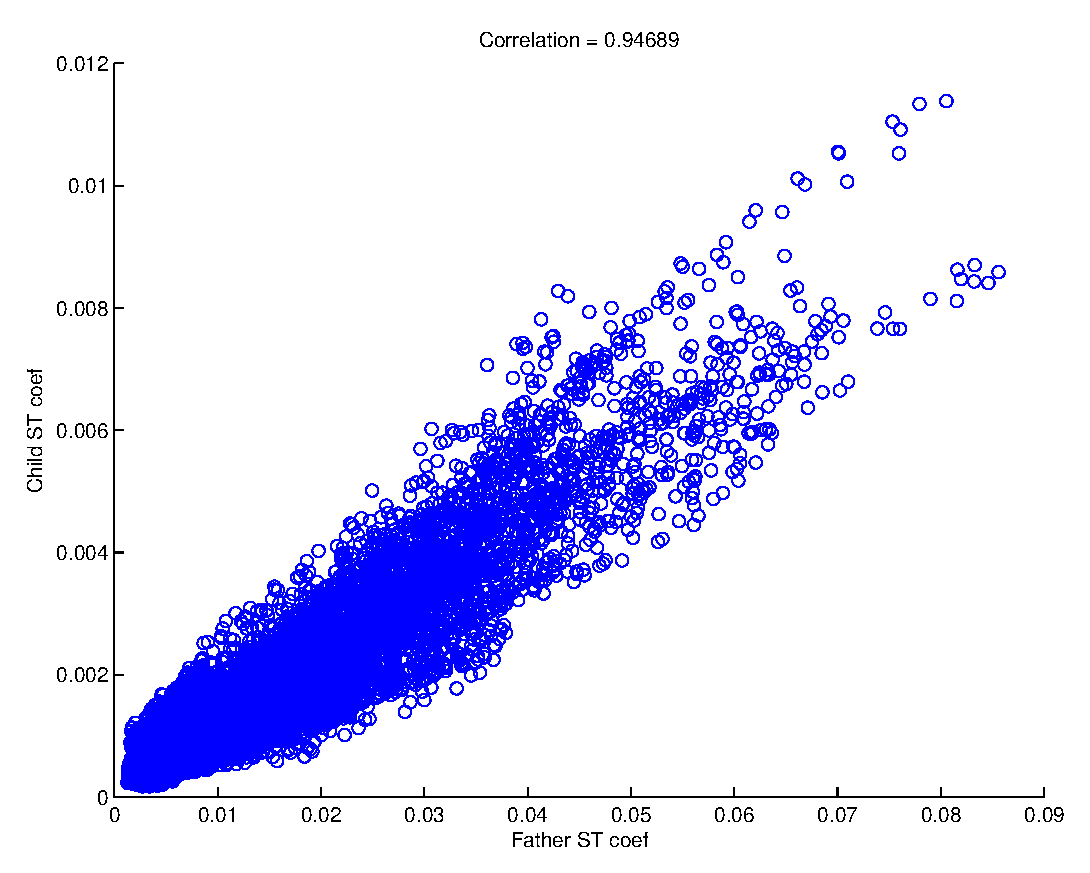
\includegraphics[height=3in]{persist_uiuc_layer2-3_highCor.eps}
						\caption{Same orientation.}%1-1-1
						\label{subfig:same orientation}
					\end{subfigure}%
					~
					\begin{subfigure}[t]{0.48\textwidth}
						\centering
						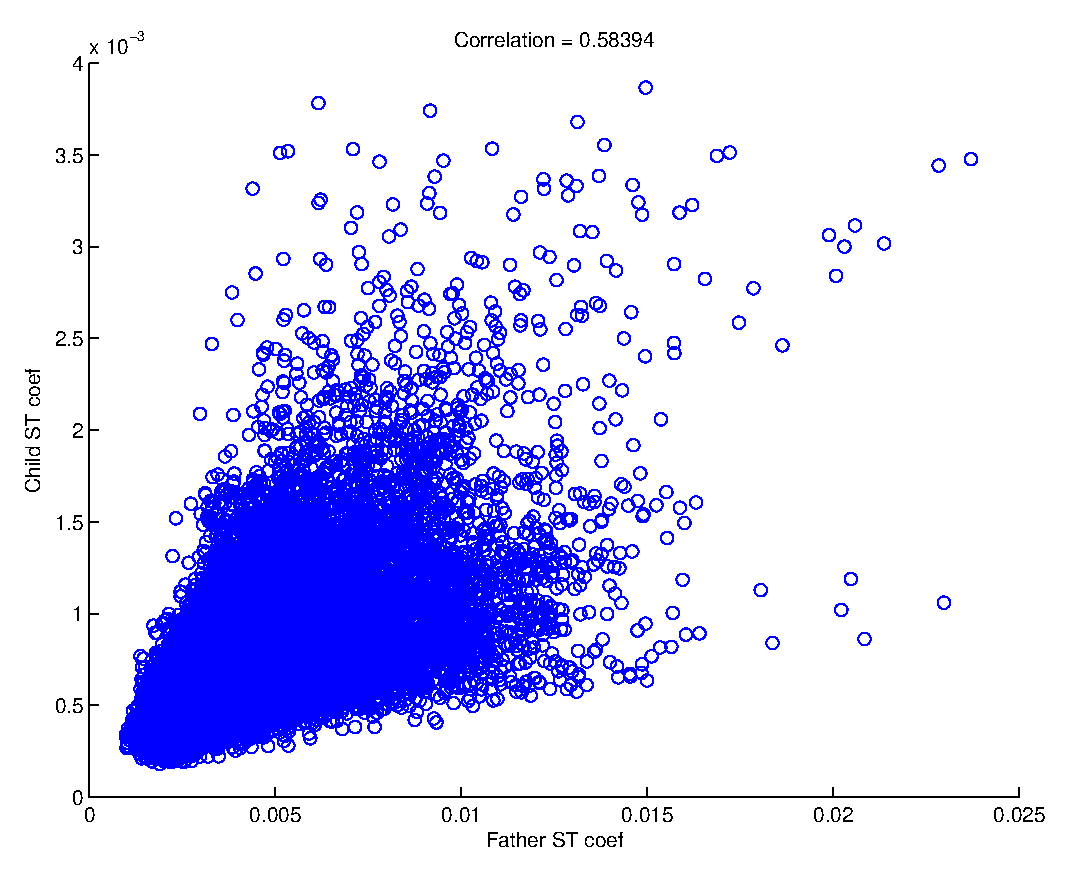
\includegraphics[height=3in]{persist_uiuc_layer2-3_lowCor.eps}
						\caption{Different orientations.} %3-1-3
						\label{subfig:dif orientation}
					\end{subfigure}%
					\caption[Persistence - Experiment 1.]{\centering Persistence - Experiment 1: Magnitude of the scattering coefficients obtain for a realization of the class ``brick wall'' of the \textit{CUReT} texture dataset at a given index $i$ of the tree against those of its father $\rho(i)$. The scattering network has $M=3$ layers, $J=4$ scales and $L=4$ orientations.}
					\label{fig:Persistence - 1}
				\end{center}
		\end{figure} 

		\begin{center}
			\begin{table}[h]
				\begin{center}				
					\begin{tabular}{|p{3cm}||p{4cm}|p{4cm}|}
						\hline
						\multicolumn{3}{|c|}{Classification results} \\
						\hline
						Signal:					&	Correlation mean	& Correlation variance	\\
						\hline
						diagonal:				& 0.909							& 0.260									\\
						Square:					& 0.811							& 0.300									\\
						Circle:					& 0.876							& 0.164									\\
						uiuc brick:			& 0.647							& 0.241									\\
						Mandrill:				& 0.503							& 0.255									\\
						Lena:						& 0.727							& 0.236									\\

						\hline
					\end{tabular}
				\end{center}
				\caption[Persistence - Experiment 2.]{\centering Persistence - Experiment 2: Average correlation across nodes of the scattering transform applied to different signals. The scattering network has $M=3$ layers, $J=4$ scales and $L=4$ orientations.}
				\label{table:Persistence - 2}
			\end{table}
		\end{center}
	
		
  \section{Learning the tree structure:}
    \label{sec:SCHMT/Learning}
    
    As seen in Section~\ref{subsec:PGMs/MM/Learning}, Hidden Markov  models can be trained using Expectation-Maximization methods. Hidden Markov chains use a version of the EM algorithm called Forward-Backward algorithm allowing the propagation of the hidden states along the chain. \citet{crouse1998wavelet} proposed the Upward-Downward algorithm, an adaptation to the hidden Markov trees of the Forward-Backward algorithm. Both algorithms were suffering from underflowing problems~\citep{ephraim2002hidden} and \citet{durand2004computational} adapted \citet{devijver1985baum} smoothing trick to create a smoothed version of the learning algorithm for trees. This section proposes our rewritten version of the smoothed EM algorithm adapted to irregular, non-homogeneous and non-binary HMTs.\\
       
    To do so one needs to introduce the following notation:\\
    \begin{itemize}
			\item $\forall i \in \mcalT$, let $n_{i}$ be the number of children of the node $i$.\\
      \item $\forall i \in \mcalT$, let $\bar{\mcalS}_{i}= \bar{s}_{i}$ be the observed sub-tree rooted at node $i$. By convention $\bar{\mcalS}_{0}$ denotes the entire observed tree.\\
      \item $\forall i \in \mcalT$, let $\bar{\mcalS}_{c(i)}= \bar{s}_{c(i)}$ be the entire -possibly empty collection of observed sub-trees rooted at the children of node $i$ (\ie the sub-tree $\bar{s}_{i}$ except its root $s_{i}$).\\
      \item If $\bar{\mcalS}_{i}$, is a sub-tree of $\bar{\mcalS}_{j}$, then $\bar{\mcalS}_{j\backslash i} = \bar{s}_{j\backslash i}$ is the sub-tree rooted at node $j$ except the sub-tree rooted at node $i$.\\
      \item $\forall i \in \mcalT$ let $\bar{\mcalS}_{0\backslash c(i)}= \bar{s}_{0\backslash c(i)}$ be the entire tree except for the sub-trees rooted at children of node $i$.\\
    \end{itemize}
    
    \begin{note}
			Those notations transpose to the hidden state and for instance $\bar{\mcalH}_{i}= \bar{h}_{i}$ is the state sub-tree rooted at node $i$.\\      
    \end{note}

    \subsection{E-Step:}
			\label{subsec:SCHMT/Learning/E}
			The smoothed version of the E-step requires the computation of the conditional probability distributions $\xi_{i}(k) = P(H_{i}=k | \bar{\mcalS}_{i}= \bar{s}_{i})$ (smoothed probability) and $P(H_{i}=k, H_{\rho(i)}=g | \bar{\mcalS}_{i}= \bar{s}_{i})$ for each node $i \in \mcalT$ and states $k$ and $g$. The smoothed probability adapted to the HMT structure can be decomposed as,
			
			\begin{equation}
			  \xi_{i}(k) = 
					\frac{P(\bar{\mcalS}_{0\backslash i}= \bar{s}_{0\backslash i} | H_{i}=k)}
						{P(\bar{\mcalS}_{0\backslash i}= \bar{s}_{i\backslash i} | \bar{\mcalS}_{1}= \bar{s}_{i})} 
					P(H_{i}= k |\bar{\mcalS}_{i}= \bar{s}_{i})
				\label{eq:Smoothed P decomposition}
			\end{equation}
			
			The smoothed upward-downward algorithm requires the introduction the following quantities,
			
			\begin{equation}
			  \beta_{i}(k) = P(H_{i}=k | \bar{\mcalS}_{i}= \bar{s}_{i})
			  \label{eq:UD beta node}
			\end{equation}
			\begin{equation}
			  \beta_{\rho(i)i}(k) = \frac{P(\bar{\mcalS}_{i}= \bar{s}_{i} | H_{\rho(i)}=k)} {P(\bar{\mcalS}_{i}= \bar{s}_{i}) }
			  \label{eq:UD beta node and parents}
			\end{equation}
						\begin{equation}
			  \alpha_{i}(k) = \frac{P(\bar{\mcalS}_{0\backslash i}= \bar{s}_{0\backslash i} | H_{\rho(i)}=k)} {P(\bar{\mcalS}_{0\backslash i}= \bar{s}_{0\backslash i} | \bar{\mcalS}_{i}= \bar{s}_{i} ) }
			  \label{eq:UD alpha}
			\end{equation}\\
			
			The smoothed upward-downward algorithm also requires the preliminary knowledge  of the marginal state distributions $P(H_{i}=k)$ for each node $i$. However this can simply be achieved by a downward recursion initialized at the root node with $P(H_{0}=k)=\pi_{0}(k)$ and then cascading the information down the tree using the recursive Formula~\ref{eq:SCHMT - State proba 1}.
			
			\subsubsection{Upward recursion:}
				\label{subsubsec:SCHMT/Learning/E/Up}
				The upward algorithm is initialized at all the leaves of the tree, by computing $\beta_{i}(k)$ using,
				
				\begin{equation}
					\begin{split}
						\beta_{i}(k)	&= P(H_{i}=k | \bar{\mcalS}_{i}= \bar{s}_{i})\\
													&= P(H_{i}=k | \mcalS_{i}= s_{i})\\
													&= \frac{P(S_{i}= s_{i} | H_{i}=k)P(H_{i}=k)} {P(S_{i}= s_{i})}\\
													&= \frac{P_{\theta_{k,i}}(s_{i}) P(H_{i}=k)} {N_{i}},
						\end{split}
						\label{eq:upward beta leaf}
				\end{equation}
				
				where the normalization factor for the leaves $N_{i}$ is given by,
				\begin{equation}
					N_{i}	= P(S_{i}= s_{i}) = \sum_{k=1}^{K} P_{\theta_{k,i}}(s_{i}) P(H_{i}=k).
					\label{eq:upward normalization leaf}
				\end{equation}
				
				Then one can recursively ---upward recursion--- compute $\beta_{i}(k)$ for the remaining nodes of the tree using,
				
				\begin{equation}
					\begin{split}
						\beta_{i}(k)	&= P(H_{i}=k | \bar{\mcalS}_{i}= \bar{s}_{i})\\
													&= \left[ \prod_{j \in c(i)} P(\bar{\mcalS}_{j}= \bar{s}_{j} | H_{i}=k) \right] P(S_{i}= s_{i} | H_{i}=k) \frac{P(H_{i}=k)} {P(\bar{\mcalS}_{i}= \bar{s}_{i})}\\
													&= \left[ \prod_{j \in c(i)}  \frac{P(\bar{\mcalS}_{j}= \bar{s}_{j} | H_{i}=k)} {P(\bar{\mcalS}_{j}= \bar{s}_{j})} \right]
														P(S_{i}= s_{i} | H_{i}=k) P(H_{i}=k) 
														\frac{\prod_{j \in c(i)} P(\bar{\mcalS}_{j}= \bar{s}_{j})} {P(\bar{\mcalS}_{i}= \bar{s}_{i})}\\
													&= \frac{ \left[ \prod_{j \in c(i)} \beta_{ij}(k) \right] P_{\theta_{k,i}}(s_{i})P(H_{i}=k)}{N_{i}},
						\end{split}
						\label{eq:upward beta node}
				\end{equation}
				
				where the normalization factor for the non-leaf nodes $N_{i}$ is given by,
				\begin{equation}
					\begin{split}
						N_{i}	&= \frac{P(\bar{\mcalS}_{i}= \bar{s}_{i})}{\prod_{j \in c(i)} P(\bar{\mcalS}_{j}= \bar{s}_{j})}\\
									&= \sum_{k=1}^{K} \left[ \prod_{j \in c(i)} \beta_{ij}(k) \right]  P_{\theta_{k,i}}(s_{i})P(H_{i}=k).
					\end{split}
					\label{eq:upward normalization others}
				\end{equation}

				For all nodes $i$, the quantities $\beta_{\rho(i)i}(k)$ can be extracted from $\beta_{i}$ using,
				
				\begin{equation}
					\begin{split}
						\beta_{\rho(i)i}(k)	&= \frac{P(\bar{\mcalS}_{i}= \bar{s}_{i} | H_{\rho(i)}=k)} {P(\bar{\mcalS}_{i}= \bar{s}_{i}) }\\
																&= \frac{ \sum_{g=1}^{K} P(\bar{\mcalS}_{i}= \bar{s}_{i} | H_{i}=g) P(H_{i}= g | H_{\rho(i)}=k)} {P(\bar{\mcalS}_{i}= \bar{s}_{i}) }\\
																&= \sum_{g=1}^{K} \frac{ P(H_{i}=g | \bar{\mcalS}_{i}= \bar{s}_{i})}{P(H_{i}=g)} P(H_{i}= g | H_{\rho(i)}=k)\\
																&= \sum_{g=1}^{K} \frac{\beta_{i}(g) \epsilon_{i}^{(kg)}}{P(H_{i}=g)}.
						\end{split}
						\label{eq:upward beta node and parents}
				\end{equation}
				
				Using those relationships, one can derive the upward Algorithm~\ref{algo:Smoothed upward}.
			
				\begin{center}
					\begin{algorithm}
						\textbf{Meta-parameters:}\\
							$K$\\
								
						\textbf{Initialization:}\\
							\tcp{$P_{\theta_{k,i}}(s_{i})$:}
							\For{All the nodes $i$ of the tree $\mcalT$}{
								$P_{\theta_{k,i}}(s_{i}) = \mcalN(s_{i} | \mu_{k,i},\sigma_{k,i})$
								}
								
							\tcp{Loop over the leaves $i$ of the tree:}
							\For{All the leaves $i$ of the tree $\mcalT$}{
								$\beta_{i}(k) = \frac{P_{\theta_{k,i}}(s_{i}) P(H_{i}=k)}{\sum_{g=1}^{K} P_{\theta_{g,i}}(s_{i}) P(H_{i}=g)}$\\
								$\beta_{i,\rho(i)}(k) = \sum_{g=1}^{K}\frac{\beta_{i}(g) \epsilon_{i}^{(kg)}}{P(H_{i}=g)} . P(H_{\rho(i)}=k)$ \\
								$l_{i} = 0$
								}
								
						\textbf{Induction:}\\
							\tcp{Bottom-Up loop over the nodes of the tree:}
							\For{All non-leaf nodes $i$ of the tree $\mcalT$}{
								$M_{i} = \sum_{k=1}^{K} P_{\theta_{k,i}}(s_{i}) \prod_{j \in c(i)} \frac{\beta_{j,i}(k)}{P(H_{i}=k)^{n_{i}-1}}$ \\
								$l_{i} = \log(M_{i}) + \sum_{j \in c(i)}l_{j}$\\
								$\beta_{i}(k) = \frac{P_{\theta_{k,i}(s_{i})} \prod_{j \in c(i)}(\beta_{j,i}(k))}{P(H_{i}=k) ^{n_{i}-1} M_{i}} $\\
								\For{All the children nodes $j$ of node $i$}{
									$\beta_{i\backslash c(i)}(k) = \frac{\beta_{i}(k)}{\beta_{i,j}(k)}$
									}
								$\beta_{i,\rho(i)}(k) = \sum_{g=1}^{K} \frac{\beta_{i}(g) \epsilon_{i}^{(kg)}}{P(H_{i}=g)} .P(H_{\rho(i)}=k)$
								}
						\caption{Smoothed upward algorithm.}
						\label{algo:Smoothed upward}		
					\end{algorithm}        
				\end{center}
				
			\subsubsection{Downward recursion:}
				\label{subsubsec:SCHMT/Learning/E/Downward}
				
				The downward recursion can either be built on the basis of the quantities $\alpha_{i}(k)$ defined in Equation~\ref{eq:UD alpha} or using the smoothed probabilities $\xi_{i}(k) = P(H_{i}=k | \bar{\mcalS}_{i}= \bar{s}_{i})$. The downward recursion on $\xi_{i}$ is initialized at the root node with,
				
				\begin{equation}
				  \xi_{0}(k)= P(H_{0}=k | \bar{\mcalS}_{0}=\bar{s}_{0}) = \beta_{0}(k).
				  \label{eq:Downward init}
				\end{equation}

				The quantities $\xi_{i}$ can then be computed recursively for each node of the tree using,
				
				\begin{equation}
					\begin{split}
						\xi_{i}(k)	&= P(H_{i}=k | \bar{\mcalS}_{0}=\bar{s}_{0}) \\
												&= \sum_{g=1}^{K} \frac{P(H_{i}=k, H_{\rho(i)}=g, \bar{\mcalS}_{0}= \bar{s}_{0})}{P(H_{\rho(i)}=g, \bar{\mcalS}_{0}= \bar{s}_{0})} P(H_{\rho(i)}=g | \bar{\mcalS}_{0}= \bar{s}_{0})\\
												&= P(\bar{\mcalS}_{i}= \bar{s}_{i} | H_{i}=k)  
													 \sum_{g=1}^{K} \frac{P(H_{i}=k | H_{\rho(i)}=g)}{P(\bar{\mcalS}_{i}= \bar{s}_{i} | H_{\rho(i)}=g)}
% 													 \frac{P(H_{\rho(i)}=g | \bar{\mcalS}_{0 \backslash i}= \bar{s}_{0 \backslash i})}{P(H_{\rho(i)}=g | \bar{\mcalS}_{0 \backslash i}= \bar{s}_{0 \backslash i})}
 													 P(H_{\rho(i)}=g | \bar{\mcalS}_{0}= \bar{s}_{0})\\
 												&= \frac{\beta_{i}(k)}{P(H_{i}=k)} \sum_{g=1}^{K} \frac{ \epsilon_{i}^{(gk)} \xi_{\rho(i)}(g)}{\beta_{\rho(i),i}(g)}.
						\end{split}
						\label{eq:Downward recursion xi}
				\end{equation}
				
				Using the fact that for all $i \in \mcalT \;\;\; \xi_{i}(k) = \beta_{i}(k)\alpha_{i}(k)$ and the relationship from Equation~\ref{eq:Downward recursion xi}, one can express the downward pass as presented in Algorithm~\ref{algo:Smoothed downward}.
    
				\begin{center}
					\begin{algorithm}
						\textbf{Meta-parameters:}\\
							$K$\\
								
						\textbf{Initialization:}\\
							$\alpha_{0}(k) = 1$
								
						\textbf{Induction:}\\
							\tcp{Top-Down loop over the nodes of the tree:}
							\For{All nodes $i$ of the tree $\mcalT\backslash\{0\}$}{
 								$\alpha_{i}(k) = \frac{1}{P(H_{i}=k)} \sum_{g=1}^{K} \alpha_{\rho(i)}(g) \epsilon_{i}^{(gk)} \beta_{\rho(i)\backslash i}(g) P(H_{\rho(i)}=g)$
								}
						\caption{Smoothed downward algorithm.}
						\label{algo:Smoothed downward}		
					\end{algorithm}        
				\end{center}
				
			\subsubsection{Conditional properties:}
				\label{subsubsec:SCHMT/Learning/E/Cond}
				
				To complete the E-step one needs to compute the conditional probabilities for each node. This is done by noticing that,
				
				\begin{equation}
				  \forall i \in \mcalT \;\;\; P(H_{i}=k | \bar{\mcalS}_{0}=\bar{s}_{0}) = \alpha_{i}(k) \beta_{i}(k),
				  \label{eq:Estep cond proba node}
				\end{equation}
				and
				\begin{equation}
				  \forall i \in \mcalT\backslash\{0\} 
				  \;\;\; P(H_{\rho(i)}=g, H_{i}=k | \bar{\mcalS}_{0}=\bar{s}_{0}) = \frac{\beta_{i}(k)\epsilon_{i}^{(gk)}\alpha_{\rho(i)}(g)\beta_{\rho(i)}(g)}{P(H_{i}=k) \beta_{\rho(i)i}(g)}.
				  \label{eq:E-step cond proba and parent}
				\end{equation}
		
		\subsection{M-Step:}
			\label{subsec:SCHMT/Learning/M}
			
			The \textit{Maximization} step of the EM algorithm aims at finding the optimum of the log-likelihood of the observations with regards to the parameters and then use those pseudo-optimal parameters for the next \textit{Expectation} step. In other words the iteration $m$ of the EM process, the M-step carries out the update,
			
			\begin{equation}
				\Theta^{m+1} = \argmax_{\Theta} \left(E[\ln f(\bfx,H|\Theta)|\bfx,\Theta^{l}] \right).
				\label{eq:Mstep argax theta}
			\end{equation}
			
			The $\Theta$ maximizing the log-likelihood in Equation~\ref{eq:Mstep argax theta} can be expressed analytically and this yields Algorithm~\ref{algo:Mstep}
			
			\begin{center}
				\begin{algorithm}
					\textbf{Meta-parameters:}\\
						$K$,\\
						Distribution family for $P_{\theta}$ \tcp*{Here Gaussian}
						$N$ \tcp*{Number of observed realizations of the signal}
							
					\textbf{Initialization:}\\
						$\pi_{0}(k) = \frac{1}{N} \sum_{n=1}^{N} P(H_{0}^{n}=m|s_{0}^{n},\Theta^{l})$
							
					\textbf{Induction:}\\
						\tcp{Loop over the nodes of the tree:}
						\For{All nodes $i$ of the tree $\mcalT\backslash\{0\}$}{
							$P(H_{i}=k) = \frac{1}{N} \sum_{n=1}^{N} P(H_{i}^{n}=k|\bar{s}_{0}^{n},\Theta^{l})$,\\
							$\epsilon_{i}^{gk} = \frac{\sum_{n=1}^{N} P(H_{i}^{n} = k, H_{\rho(i)}^{n}=g |\bar{s}_{0}^{n}, \Theta^{l})} {N P(H_{\rho(i)}=k)}$,\\
							$\mu_{k,i} = \frac{\sum_{n=1}^{N} s_{i}^{n} P(H_{i}^{n} = k |\bar{s}_{0}^{n}, \Theta^{l})} {N P(H_{i}=k)}$,\\
							$\sigma_{k,i}^{2} = \frac{\sum_{n=1}^{N} (s_{i}^{n} - \mu_{k,i})^{2} P(H_{i}^{n} = k |\bar{s}_{0}^{n}, \Theta^{l})} {N P(H_{i}=k)}$.\\
							}
					\caption{M-step of the EM algorithm.}
					\label{algo:Mstep}
				\end{algorithm}        
			\end{center}
			
		\subsection{EM algorithm:}
			\label{subsec:SCHMT/Learning/EM}
			
			Finally the EM algorithm iterates over the \textit{E-step} and the \textit{M-step} as described by Algorithm~\ref{algo:EM}.
			
			\begin{center}
				\begin{algorithm}
					\textbf{Meta-parameters:}\\
						$K$;\\
						Distribution family for $P_{\theta}$;\\
						Convergence criteria \tcp*{Iteration limit or information based}
						Initialization method for $\Theta$ \tcp*{Random or prior knowledge}
						
					\textbf{Initialization:}\\
						$l=0$ \tcp*{Iteration counter}
						$\text{Initialize}(\Theta)$
					
					\textbf{Iteration:}\\
					\While{Not convergence}{
						\textbf{E-step:} Calculate $P(\bar{\mcalH}|\bar{\mcalH}, \Theta^{l})$.\\
						\textbf{M-step:} Set $\Theta^{m+1} = \argmax_{\Theta} \left(E[\ln f(\bfx,H|\Theta)|\bfx,\Theta^{l}] \right)$.\\
						l = l+1
						}
					\caption{EM algorithm.}
					\label{algo:EM}
				\end{algorithm}        
			\end{center}
			    
  \section{Classification:}
    \label{sec:SCHMT/Clf}
    
    Let $\Theta_{c}$ now be a set of parameters for an SCHMT $\mcalT$ learned using the EM algorithm described in Section~\ref{sec:SCHMT/Learning} on a training set $\{\bar{S}_{0,c}^n\}_{n \in \llbracket1, N \rrbracket} = \{ST_{(\psi, J, M, L)}(\bfx_{c}^{n})\}_{n \in \llbracket1, N \rrbracket}$ composed of the scattering representations of $N$ realizations of a signal of class $c$ . Let also $\bfx^{new}$ be another realization of this signal, not used for training and $\mcalT^{new}$ be the instance of the SCHMT generated by this realization.\\
    
    In this context the MAP algorithm aims at finding the optimal hidden tree $\hat{\bar{h}}_{0}^{new}=(\hat{h}_{0}^{new} \dots \hat{h}_{I-1}^{new})$ maximizing the probability of this sequence given the model's parameters $P(\bar{\mcalH}_{0}= \hat{\bar{h}}_{0}^{new}|\mcalT^{new},\Theta_{c})$. The MAP framework also provides $\hat{P}$ the value of this maximum.\\
    
    For SCHMT the MAP algorithm has the form described by Algorithm~\ref{algo:MAP}.
    
		\begin{center}
			\begin{algorithm}
				\textbf{Meta-parameters:}\\
					$K$;\\
					
				\textbf{Initialization:}\\
					\For{all leaves $i$ of $\mcalT$}{
						$\gamma_{i}(k) = \beta_{i}(k)$ \tcp*{The gamma for all $k$ must be computed before the next step}
						$\gamma_{i,\rho(i)}(k) = \max_{1\leq g \leq K} \gamma_{i}(g)\epsilon_{i}^{kg}$ \\
						$\xi_{i}(k) = \argmax_{1\leq g\leq K} \gamma_{i}(g)\epsilon_{i}^{kg}$\\
					}
					
				\textbf{Induction:}\\
					\tcp{Top-Down loop over the nodes of the tree:}
					\For{All nodes $i$ of the tree $\mcalT\backslash\{0\}$}{					
						$\gamma_{i}(k) = P_{\theta_{k,i}}(s_{i}) \prod_{j \in c(i)} \gamma_{j,i}(k)$\\
						$\gamma_{i,\rho(i)}(k) = \max_{1\leq g \leq K} \gamma_{i}(g)\epsilon_{i}^{kg}$ \tcp*{Except at root node}
						$\xi_{i}(k) = \argmax_{1\leq g\leq K} \gamma_{i}(g)\epsilon_{i}^{kg}$\\
					}
				
				\textbf{Termination:}\\
					$\hat{P} = \max_{1\leq g \leq K} \gamma_{0}(g)$\\
					$\hat{h}_{0} = \argmax_{1\leq g \leq K} \gamma_{0}(g)$\\
				
				\textbf{Downward tracking:}\\
					\tcp{Creation of the hidden tree from the root node}
					\For{All nodes $i$ of the tree $\mcalT\backslash\{0\}$}{
						$\hat{h}_{i}=\xi_{i}(\hat{h}_{\rho(i)})$
					}
				
				\caption{MAP algorithm.}
				\label{algo:MAP}
			\end{algorithm}        
		\end{center}
		
		The MAP Algorithm~\ref{algo:MAP} can be used in a multi-class classification problem by training an SCHMT model per class and then when presented with a new realization $\bfx^{new}$ comparing the probability of the MAP hidden tree provided by each model as described by Algorithm~\ref{algo:MAP clf}.
		
		\begin{center}
			\begin{algorithm}
				\textbf{Meta-parameters:}\\
					$K$; $C$ \tcp*{Number of classes}
					
				\For{All classes $c$}{
					$\hat{P}_{c} = \text{MAP}(\bfx^{new},\Theta_{c},K)$\\
				}
				
				$\hat{P}= \max_{0\leq c < C} \hat{P}_{c}$\\
				$l= \argmax_{0\leq c < C} \hat{P}_{c}$\\
				
				\caption{MAP algorithm applied to multi-class classification problem.}
				\label{algo:MAP clf}
			\end{algorithm}        
		\end{center}
    
%%%%%%%%%%%%%%%%%%%%%%%%%%%%%%%%%%%%%%%%%%%%%%%%%%%%%%%%%%%%%%%%%%%%%%%%%%%%%%%%%%%%%%%%%%%%%%%%%%%%%%%%%%%%%%%%%%%%%%%%%%%%%%%%%%%%%%%%%%%%%%%%%%%%%%%%%%%%%%%%%%%%%%%%%%%%%%%%%%%%%%%%%%%%%%%%%%%%%%%%%%%%%%%%%%%%%%%%%%%%%
%%%%%%%%%%%%%%%%%%%%%%%%%%%%%%%%%%%%%%%%%%%%%%%%%%%%%%%%%%%%%%%%%%%%%%%%%%%%%%%%%%%%%%%%%%%%%%%%%%%%%%%%%%%%%%%%%%%%%%%%%%%%%%%%%%%%%%%%%%%%%%%%%%%%%%%%%%%%%%%%%%%%%%%%%%%%%%%%%%%%%%%%%%%%%%%%%%%%%%%%%%%%%%%%%%%%%%%%%%%%%
%%%%%%%%%%%%%%%%%%%%%%%%%%%%%%%%%%%%%%%%%%%%%%%%%%%%%%%%%%%%%%%%%%%%%%%%%%%%%%%%%%%%%%%%%%%%%%%%%%%%%%%%%%%%%%%%%%%%%%%%%%%%%%%%%%%%%%%%%%%%%%%%%%%%%%%%%%%%%%%%%%%%%%%%%%%%%%%%%%%%%%%%%%%%%%%%%%%%%%%%%%%%%%%%%%%%%%%%%%%%%
\chapter{Experimental results:}
  \label{chap:Exp}
  This section presents some experimental results obtained using scattering convolutional hidden Markov trees for classification tasks. First SCHMT are applied to classify seabed and ripples in sonar imagery. Then this model is adapted to perform a very naive segmentation on a sonar imagery.
  
%   \section{Shapes:}
% 		\label{sec:Exp/Shape:}
% 		
% 		The SCHMT performance on classification tasks are at first assessed on telling apart different geometrical shapes. The data are noisy and translated realizations of two signals. The first signal is an $100$ by $100$ binary image picturing a centered black square on a white background. Examples of this class can be seen in Figure~\ref{fig:Shape square}. The second class is a $100$ by $100$ binary image picturing a centered black triangle on a white background. Examples of this class can be seen in Figure~\ref{fig:Shape triangle}. 
% 		
% 		\begin{figure}
% 			\begin{center}
% 				
\includegraphics[width=3.5in]{placeholder.jpg}
% 			  \caption[Shape classification: square]{(a) Orignial signal (b) realization}
% 			  \label{fig:Shape square}
% 			\end{center}
% 		\end{figure}
% 		
% 		\begin{figure}
% 			\begin{center}
% 				
\includegraphics[width=3.5in]{placeholder.jpg}
% 			  \caption[Shape classification: triangle]{(a) Orignial signal (b) realization}
% 			  \label{fig:Shape triangle}
% 			\end{center}
% 		\end{figure}

% 		
  \section{Sonar Imagery:}
		\label{sec:Exp/Sonar:}
		
		In underwater mine detection recovering a large proportion of the true positives is crucial since missing one of them could be very costly. However, recovering a large proportion of the true positives may incur many false positives. Reducing these to a manageable number is an open problem in marine sciences. Indeed by its design an underwater mine can be mistaken with some natural features of the seabed. One of those natural features generating many false alarm are called ``ripple''. Those regular patterns drawn in the sand by currents can vary greatly in shape and orientation. To reduce the number of false positive it is thus interesting to be able to tell apart flat seabed from ripply one. This is the task proposed for the SCHMT.\\
		
		The data used are extracted from the \textit{UDRC MCM} sonar imagery dataset~\citep{udrc2015sonar}. This dataset comprises Synthetic Aperture RADAR (SAS imagery) and hyperspectral data ---not used in this experiment. From those very high dimensional images, $100$ by $100$ patches have been extracted and labelled as either seabed or ripple (see respectively Figure~\ref{fig:Seabed patch} and Figure~\ref{fig:Ripple patch}). The classification task at hand is very challenging due to the low informative content of each images and the high intra-class variability.\\

		\begin{figure}[h]
			\centering
			\begin{subfigure}[t]{0.3\textwidth}
				\centering
				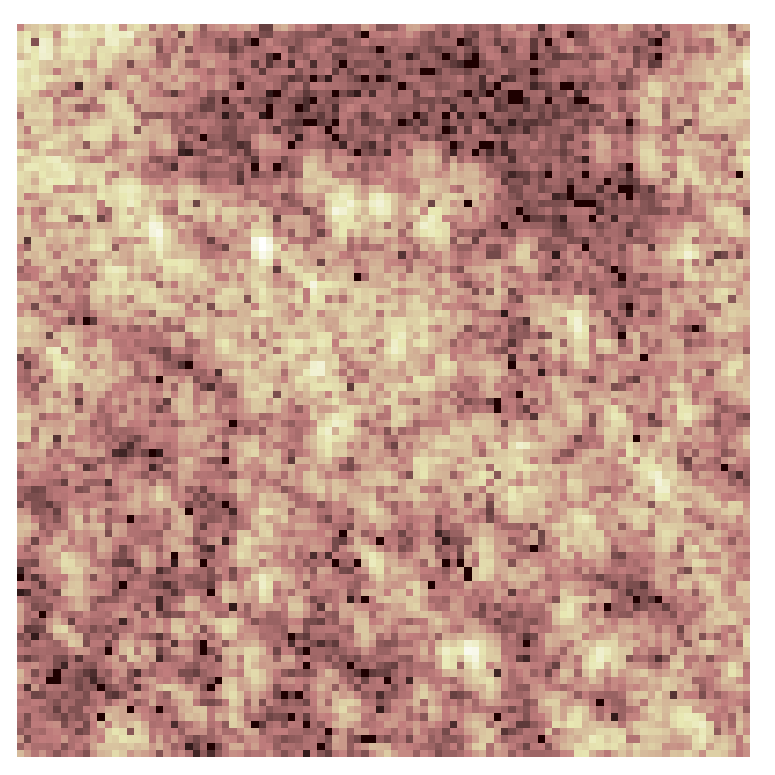
\includegraphics[height=1.8in]{patch_seabed_1.eps}
			\end{subfigure}%
			~ 
			\begin{subfigure}[t]{0.3\textwidth}
        \centering
        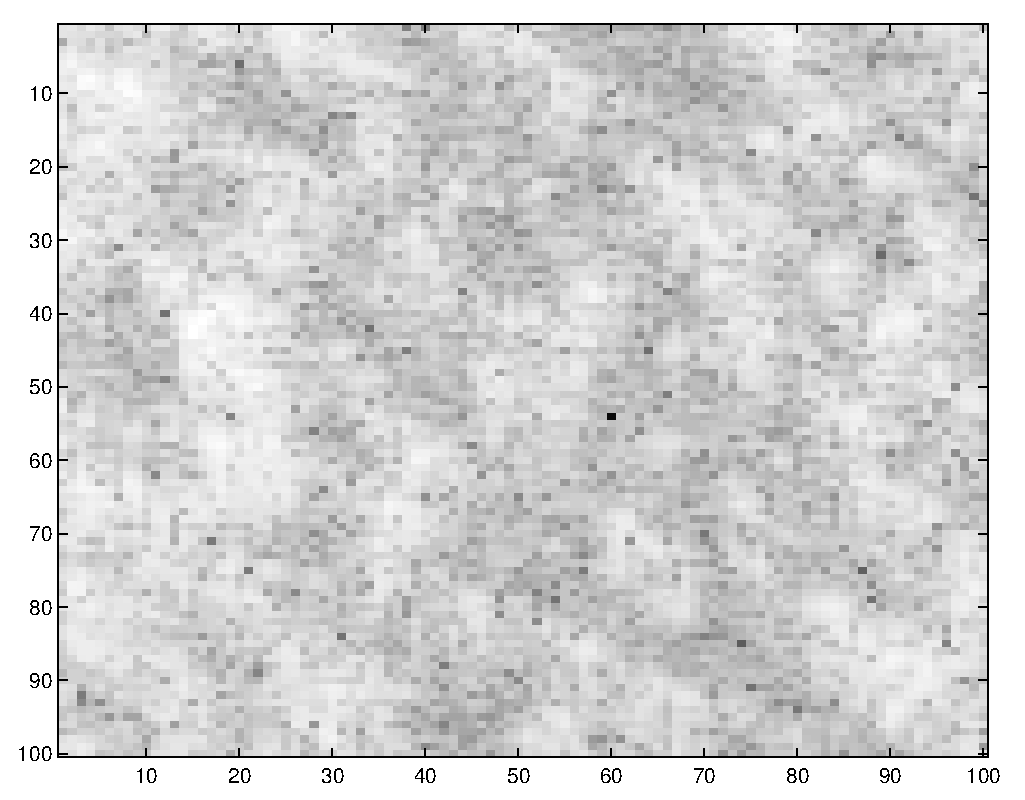
\includegraphics[height=1.8in]{patch_seabed_2.eps}
			\end{subfigure}
			~
			\begin{subfigure}[t]{0.3\textwidth}
        \centering
        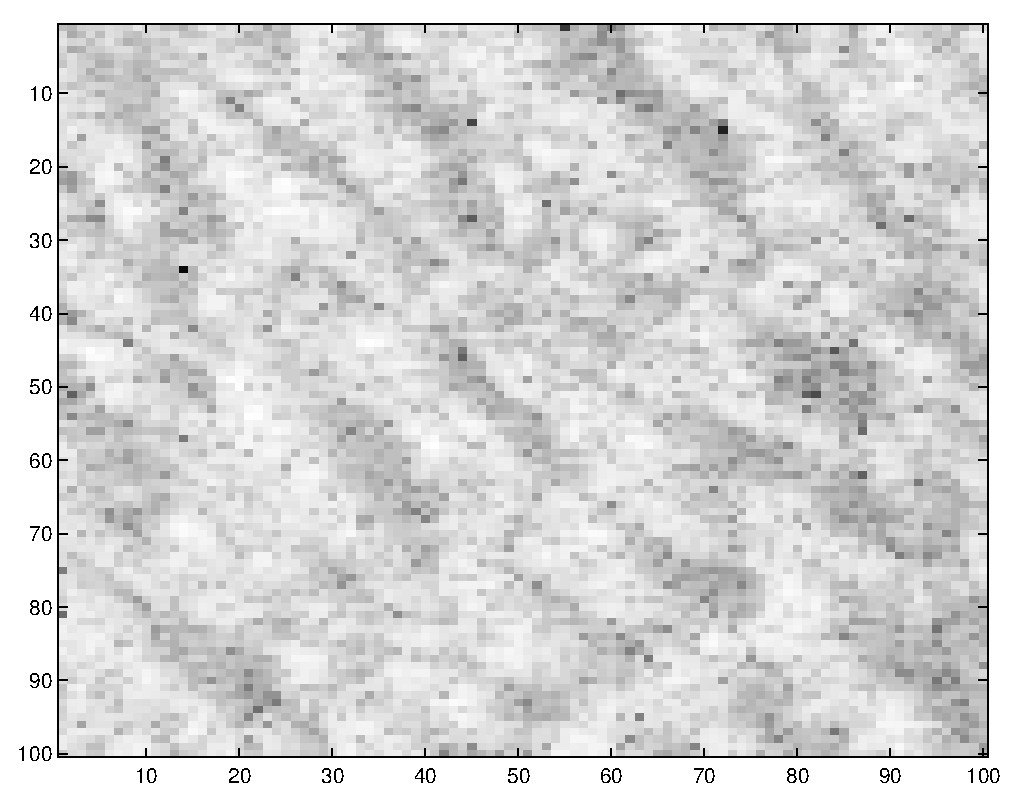
\includegraphics[height=1.8in]{patch_seabed_3.eps}
			\end{subfigure}
			\caption{Sample of seabed patches.}
			\label{fig:Seabed patch}
		\end{figure}
		
		
		\begin{figure}[h]
			\centering
			\begin{subfigure}[t]{0.3\textwidth}
				\centering
				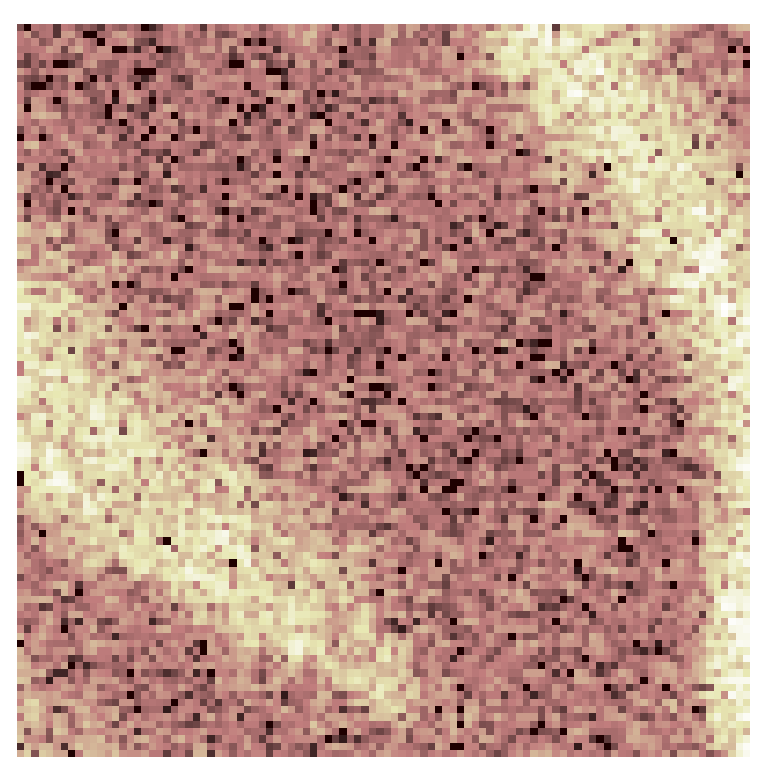
\includegraphics[height=1.8in]{patch_ripple_1.eps}
			\end{subfigure}%
			~ 
			\begin{subfigure}[t]{0.3\textwidth}
        \centering
        \includegraphics[height=1.8in]{patch_ripple_2.eps}
			\end{subfigure}
			~
			\begin{subfigure}[t]{0.3\textwidth}
        \centering
        \includegraphics[height=1.8in]{patch_ripple_3.eps}
			\end{subfigure}
			\caption{Sample of ripple patches.}
			\label{fig:Ripple patch}
		\end{figure}
		
		The scattering transform used has $M=3$ orders, $J=5$ scales, $L=3$ orientations and uses a Morlet wavelet and the hidden Markov tree has $K=2$ states and is using a mixture of Gaussian to describe the relationship between the scattering coefficients and the hidden states. Two models ---one for each class considered--- $\Theta_{ripple}$ and $\Theta_{seabed}$ are trained on $200$ realizations of their class signal. The testing is then realized on $80$ images ---$40$ of each classes. The performance of the SCHMT are assessed on $100$ instances of this experiment and the results are displayed in Table~\ref{table:Clf_ripple}.\\
		
		\begin{center}
			\begin{table}[h]
				\begin{center}				
					\begin{tabular}{ |p{3cm}||p{2cm}|p{2cm}|p{2cm}|p{2cm}|p{2cm}| }
						\hline
						\multicolumn{6}{|c|}{Classification results} \\
						\hline
						Classification score:	&	N			& Mean	& Variance	& Maximum	& Minimum \\
						\hline
						Full:									& 100   & 0.74	& 0.101			& 0.9				&	0.5\\
						$\geq 60\%$: 					& 91    & 0.76	& 0.079			& 0.9				&	0.6\\
						$\geq 70\%$: 					& 73    & 0.79	& 0.058			& 0.9				&	0.7\\
						\hline
					\end{tabular}
				\end{center}
				\caption{Classification performance over $100$ experiments of Ripple/Seabed classification.}
				\label{table:Clf_ripple}
			\end{table}
		\end{center}
		
		The first line of Table~\ref{table:Clf_ripple} displays the results obtained on the all $100$ experiments run. Despite a slightly unsatisfying average  classification score of $74\%$, the best models reach a good accuracy of $90\%$. The lowest score is $50\%$ accuracy and is obtained because all the testing examples are associated with to one class. This can be explained by one class's model having reached a local maxima way less interesting than the other. Those results highly a weakness of the current learning method. At the moment the convergence is not properly tested during the learning phase. However this experiment and its very satisfying best model also validate the assumptions made since when the convergence occurs correctly the discriminative performance are good. The other lines in Table~\ref{table:Clf_ripple} simulates the results if a validation criterion based on an imposed accuracy score on a validation set was imposed. This validation set would be a way to address the problem of occasional convergence to a local minima. Another leads would be to work on the EM algorithm itself to make it more robust by adding information based convergence test.  
		
  \section{Segmentation:}
		\label{sec:Exp/Segmentation:}
		
		On its simplest form  a segmentation task can be seen as a set of independent classification tasks on subpart of an image. Hence one can use the models trained in the previous section to realize the segmentation of a full sonar imagery.\\
		
		One of the  $2000 \times 7300$ image from the \textit{UDRC MCM} is cut into a set $100 \times 100$ patches ---some regions of the original image are not considered. And each of those patches is presented to the classifier. Results of this procedure can be seen in Figure~\ref{fig:Segmentation}.\\

		\begin{figure}[h]
			\centering
			\begin{subfigure}[t]{0.48\textwidth}
				\centering
				\includegraphics[height=1.8in]{seg_original.eps}
				\caption{Original image}
			\end{subfigure}%
			~ 
			\begin{subfigure}[t]{0.48\textwidth}
        \centering
        \includegraphics[height=1.8in]{seg_result.eps}
        \caption{Segmentation}
			\end{subfigure}
			\\
			~
			\begin{subfigure}[t]{0.48\textwidth}
        \centering
        \includegraphics[height=1.8in]{seg_pmap_seabed.eps}
        \caption{Probability map for the class ''seabed''}
        \label{subfig:seg_pmap_seabed}
			\end{subfigure}
			~
			\begin{subfigure}[t]{0.48\textwidth}
        \centering
        \includegraphics[height=1.8in]{seg_pmap_ripple.eps}
        \caption{Probability map for the class ''ripple''}
        \label{subfig:seg_pmap_ripple}
			\end{subfigure}
			~
			\caption{Segmentation of a sonar imagery.}
			\label{fig:Segmentation}
		\end{figure}
		
		Even though this approach to segmentation is very naive and does not introduce any form of spatial smoothing or correlation between nearby patches to improve accuracy, the SCHMT model provides satisfying segmentation of the seabed. Furthermore, as displayed by the Figure~\ref{subfig:seg_pmap_ripple} and~\ref{subfig:seg_pmap_seabed}, it provides a probability map for the confidence in our segmentation decision. Those probability maps are very interesting as they show that the misclassified patches do not have a high probability of belonging to the wrong class. It just appears that given the learned model their probability to belong to their own class is very low. %Such maps are interesting as they could easily be exploited by a human operator to help in a decision taking process.
		
		
%%%%%%%%%%%%%%%%%%%%%%%%%%%%%%%%%%%%%%%%%%%%%%%%%%%%%%%%%%%%%%%%%%%%%%%%%%%%%%%%%%%%%%%%%%%%%%%%%%%%%%%%%%%%%%%%%%%%%%%%%%%%%%%%%%%%%%%%%%%%%%%%%%%%%%%%%%%%%%%%%%%%%%%%%%%%%%%%%%%%%%%%%%%%%%%%%%%%%%%%%%%%%%%%%%%%%%%%%%%%%
%%%%%%%%%%%%%%%%%%%%%%%%%%%%%%%%%%%%%%%%%%%%%%%%%%%%%%%%%%%%%%%%%%%%%%%%%%%%%%%%%%%%%%%%%%%%%%%%%%%%%%%%%%%%%%%%%%%%%%%%%%%%%%%%%%%%%%%%%%%%%%%%%%%%%%%%%%%%%%%%%%%%%%%%%%%%%%%%%%%%%%%%%%%%%%%%%%%%%%%%%%%%%%%%%%%%%%%%%%%%%
%%%%%%%%%%%%%%%%%%%%%%%%%%%%%%%%%%%%%%%%%%%%%%%%%%%%%%%%%%%%%%%%%%%%%%%%%%%%%%%%%%%%%%%%%%%%%%%%%%%%%%%%%%%%%%%%%%%%%%%%%%%%%%%%%%%%%%%%%%%%%%%%%%%%%%%%%%%%%%%%%%%%%%%%%%%%%%%%%%%%%%%%%%%%%%%%%%%%%%%%%%%%%%%%%%%%%%%%%%%%%
\chapter{Conclusion:}
	\label{chap:ccl}

  \section{Scattering convolutional hidden Markov tree:}
		This document introduces a framework to process a high-dimensional signal from the raw data to the prediction task. First SCHMTs project the data into a representational space of even higher dimensionality but of reduced volume along the invariants in the data. Then a probabilistic graphical model ---hidden Markov tree--- is used to create a generative model of the distribution of the data in this space. This model can then be used for inference tasks such as prediction.\\
  
		SCHMT appears to be a powerful tool combining the interesting properties of the scattering transform for signal representation and the representational power of the hidden Markov models. As seen in Section~\ref{chap:Exp}, the modelled distribution can be used to perform efficient discrimination/classification tasks on images with low informative content. Even though this document considers only classification, a generative model is much more versatile than a simple ---yet efficient--- discriminative counterpart. Because they model the full distribution of the data they can express more complex relationships between the observed and the unknown variables than simple discrimination (see Sub-section~\ref{subsec:PGMs/BN/Inference} for more details).
  
  %It provides with an analytically tractable interesting representation of high-dimensional signals as well as method to model the distribution of this representation. 
    
  \section{Future work:}
		Despite showing good performance when the learning phase has converged properly, SCHMT's performance is still undermined by occasional convergence issues which have drastic effects on learning quality. This observation is one of the main drivers for the upcoming work. The other main focuses are to keep a well define probabilistic framework in order to be able to express the uncertainty of our model and of our predictions.\\
		
		The version of the EM algorithm considered in this report uses full Bayesian inference. However this methods is computationally expensive and sometimes yields a poor learning. Furthermore this version of the EM algorithm provides only a point-wise estimate of the model's parameters. It would be interesting to apply variational methods the this problem~\citep{wainwright2008graphical}. Beside a potential improvement of the learning /performance, variational inference would also provide an estimated distribution for the model's parameters, allowing us to have access to a measure of uncertainty for the learned model and thus discard models according to the uncertainty on their parameters.\\
		
		Another interesting direction to follow for future works is to integrate the scattering convolutional hidden Markov tree into a hierarchical graphical models~\citep{fine1998hierarchical}. This framework would allow the use the SCHMT model as a node of a wider probabilistic graphical model. Using such an architecture yields a tremendous number of possibilities. The performance in the segmentation task could be improved by adding a layer of graphical model encoding the spatial dependencies between the different labels in the scene. One could also use hierarchical models to describe a network of sensors each providing information on a targeted scene or integrate multiple source of information into the final prediction.\\
		
		Finally another interesting lead would be to consider other architectures for the graphical model and even make it includes the representation learning step. This would be possible using Bayesian neural networks and probabilistic back-propagation~\citep{hernandez2015probabilistic} or a Bayesian flavour of back-propagation~\citep{blundell2015weight}.
    
%%%%%%%%%%%%%%%%%%%%%%%%%%%%%%%%%%%%%%%%%%%%%%%%%%%%%%%%%%%%%%%%%%%%%%%%%%%%%%%%%%%%%%%%%%%%%%%%%%%%%%%%%%%%%%%%%%%%%%%%%%%%%%%%%%%%%%%%%%%%%%%%%%%%%%%%%%%%%%%%%%%%%%%%%%%%%%%%%%%%%%%%%%%%%%%%%%%%%%%%%%%%%%%%%%%%%%%%%%%%%
%%%%%%%%%%%%%%%%%%%%%%%%%%%%%%%%%%%%%%%%%%%%%%%%%%%%%%%%%%%%%%%%%%%%%%%%%%%%%%%%%%%%%%%%%%%%%%%%%%%%%%%%%%%%%%%%%%%%%%%%%%%%%%%%%%%%%%%%%%%%%%%%%%%%%%%%%%%%%%%%%%%%%%%%%%%%%%%%%%%%%%%%%%%%%%%%%%%%%%%%%%%%%%%%%%%%%%%%%%%%%
%%%%%%%%%%%%%%%%%%%%%%%%%%%%%%%%%%%%%%%%%%%%%%%%%%%%%%%%%%%%%%%%%%%%%%%%%%%%%%%%%%%%%%%%%%%%%%%%%%%%%%%%%%%%%%%%%%%%%%%%%%%%%%%%%%%%%%%%%%%%%%%%%%%%%%%%%%%%%%%%%%%%%%%%%%%%%%%%%%%%%%%%%%%%%%%%%%%%%%%%%%%%%%%%%%%%%%%%%%%%%
\chapter{Acknowledgements:}
	We would like to thanks Dstl and UCL for their support on this project. Jean-Baptiste Regli is funded by a Dstl/UCL Impact studentship. Members from DSTL also provided useful insights on the weakness of the actual classification and segmentation tools as well as a fresh look to the work done.\\

	
%%%%%%%%%%%%%%%%%%%%%%%%%%%%%%%%%%%%%%%%%%%%%%%%%%%%%%%%%%%%%%%%%%%%%%%%%%%%%%%%%%%%%%%%%%%%%%%%%%%%%%%%%%%%%%%%%%%%%%%%%%%%%%%%%%%%%%%%%%%%%%%%%%%%%%%%%%%%%%%%%%%%%%%%%%%%%%%%%%%%%%%%%%%%%%%%%%%%%%%%%%%%%%%%%%%%%%%%%%%%%
%%%%%%%%%%%%%%%%%%%%%%%%%%%%%%%%%%%%%%%%%%%%%%%%%%%%%%%%%%%%%%%%%%%%%%%%%%%%%%%%%%%%%%%%%%%%%%%%%%%%%%%%%%%%%%%%%%%%%%%%%%%%%%%%%%%%%%%%%%%%%%%%%%%%%%%%%%%%%%%%%%%%%%%%%%%%%%%%%%%%%%%%%%%%%%%%%%%%%%%%%%%%%%%%%%%%%%%%%%%%%
%%%%%%%%%%%%%%%%%%%%%%%%%%%%%%%%%%%%%%%%%%%%%%%%%%%%%%%%%%%%%%%%%%%%%%%%%%%%%%%%%%%%%%%%%%%%%%%%%%%%%%%%%%%%%%%%%%%%%%%%%%%%%%%%%%%%%%%%%%%%%%%%%%%%%%%%%%%%%%%%%%%%%%%%%%%%%%%%%%%%%%%%%%%%%%%%%%%%%%%%%%%%%%%%%%%%%%%%%%%%%
%%%%%%%%%%%%%%%%   
% Bibliography %
%%%%%%%%%%%%%%%%
\renewcommand\bibname{Bibliography:}
\bibliographystyle{apalike}%plainnat}
\bibliography{bib_SCHMT}
% this shows references stored in the bib_SCHMT.bib file
\nocite{*}

%%%%%%%%%%%%%%%%%%%%%%%%%%%%%%%%%%%%%%%%%%%%%%%%%%%%%%%%%%%%%%%%%%%%%%%%%%%%%%%%%%%%%%%%%%%%%%%%%%%%%%%%%%%%%%%%%%%%%%%%%%%%%%%%%%%%%%%%%%%%%%%%%%%%%%%%%%%%%%%%%%%%%%%%%%%%%%%%%%%%%%%%%%%%%%%%%%%%%%%%%%%%%%%%%%%%%%%%%%%%%
%%%%%%%%%%%%%%%%%%%%%%%%%%%%%%%%%%%%%%%%%%%%%%%%%%%%%%%%%%%%%%%%%%%%%%%%%%%%%%%%%%%%%%%%%%%%%%%%%%%%%%%%%%%%%%%%%%%%%%%%%%%%%%%%%%%%%%%%%%%%%%%%%%%%%%%%%%%%%%%%%%%%%%%%%%%%%%%%%%%%%%%%%%%%%%%%%%%%%%%%%%%%%%%%%%%%%%%%%%%%%
%%%%%%%%%%%%%%%%%%%%%%%%%%%%%%%%%%%%%%%%%%%%%%%%%%%%%%%%%%%%%%%%%%%%%%%%%%%%%%%%%%%%%%%%%%%%%%%%%%%%%%%%%%%%%%%%%%%%%%%%%%%%%%%%%%%%%%%%%%%%%%%%%%%%%%%%%%%%%%%%%%%%%%%%%%%%%%%%%%%%%%%%%%%%%%%%%%%%%%%%%%%%%%%%%%%%%%%%%%%%%
%%%%%%%%%%%%%%%%%%%%%%%%%%%%%%%%%%%%%%%%%%%%%%%%%%%%%%%%%%%%%%%%%%%%%%%%%%%%%%%%%%%%%%%%%%%%%%%%%%%%%%%%%%%%%%%%%%%%%%%%%%%%%%%%%%%%%%%%%%%%%%%%%%%%%%%%%%%%%%%%%%%%%%%%%%%%%%%%%%%%%%%%%%%%%%%%%%%%%%%%%%%%%%%%%%%%%%%%%%%%%
%%%%%%%%%%%%%%%%%%%%%%%%%%%%%%%%%%%%%%%%%%%%%%%%%%%%%%%%%%%%%%%%%%%%%%%%%%%%%%%%%%%%%%%%%%%%%%%%%%%%%%%%%%%%%%%%%%%%%%%%%%%%%%%%%%%%%%%%%%%%%%%%%%%%%%%%%%%%%%%%%%%%%%%%%%%%%%%%%%%%%%%%%%%%%%%%%%%%%%%%%%%%%%%%%%%%%%%%%%%%%
% THE END
\end{document}